\documentclass[11pt,twoside,openright]{book}

% =============================================
% 1. PRE-CORE STRUCTURAL EXTENSIONS (CRITICAL ORDER)
% =============================================
\usepackage{xr-hyper} 

% =============================================
% 2. MATH, FONTS & CORE TYPOGRAPHY (Load early!)
% =============================================
\usepackage{amsmath,amssymb}
\usepackage{lmodern}

% =============================================
% 3. HYPERREF AND METADATA EXTENSIONS
% =============================================
\PassOptionsToPackage{unicode,hidelinks,colorlinks=false}{hyperref}
\PassOptionsToPackage{hyphens}{url}
\usepackage{hyperref}
\usepackage{bookmark}
\urlstyle{same} % disable monospaced font for URLs

% =============================================
% 4. THE CUSTOM TRILOGY CORE
% =============================================
\usepackage{trilogy_macros} 
\usepackage{subfiles}    

% =============================================
% 5. STANDARD SCHOLARLY PACKAGES
% =============================================
\usepackage{graphicx}
\graphicspath{{figures/}}

\usepackage{orcidlink}
\usepackage{authblk}
\usepackage{lipsum}
\usepackage[shortlabels]{enumitem}

\usepackage{algorithm}
\usepackage{algorithmic}

\usepackage{xcolor}
\usepackage{longtable,booktabs,array}
\usepackage{calc}          % for calculating minipage widths
\usepackage{etoolbox}

% =============================================
%  STANDARD SCHOLARLY PACKAGES
% =============================================
% \usepackage{microtype} 
% \UseMicrotypeSet[protrusion]{basicmath} 

% \PassOptionsToPackage{document}{ragged2e} 
% \usepackage{ragged2e}



% ============================================================
% KDP HARDCOVER TRIM / MIRRORED MARGINS / NO INTERIOR BLEED
% If trilogy_macros.sty already loads geometry, reuse that instance.
% ============================================================
\makeatletter
\@ifpackageloaded{geometry}{}{\RequirePackage{geometry}}
\makeatother
\geometry{
    paperwidth=6in,
    paperheight=9in,
    inner=0.75in,
    outer=0.625in,
    top=0.80in,
    bottom=0.80in,
    headheight=14pt,
    headsep=0.22in,
    footskip=0.35in
}

% =============================================
% 7. TYPOGRAPHIC AND PAGE LAYOUT CONFIGURATION
% =============================================
\usepackage{fancyhdr}

\fancypagestyle{plain}{
    \fancyhf{}
    \fancyhead[LE,RO]{\thepage}
    \renewcommand{\headrulewidth}{0pt}
}
\pagestyle{fancy}
\fancyhf{}
\fancyhead[LE,RO]{\thepage}
\renewcommand{\headrulewidth}{0pt}
\setlength{\headheight}{14pt}

% ============================================ 
% PANDOC COMPATIBILITY LAYER
% ============================================ 
\ifPDFTeX
  \usepackage[T1]{fontenc}
  \usepackage[utf8]{inputenc}
  \usepackage{textcomp}         
\else                           
  \usepackage{unicode-math}
  \defaultfontfeatures{Scale=MatchLowercase}
  \defaultfontfeatures[\rmfamily]{Ligatures=TeX,Scale=1}
\fi

\makeatletter
\@ifundefined{KOMAClassName}{%
  \IfFileExists{parskip.sty}{%
    \usepackage{parskip}
  }{%
    \setlength{\parindent}{0pt}
    \setlength{\parskip}{6pt plus 2pt minus 1pt}}
}{%
  \KOMAoptions{parskip=half}}
\makeatother

\makeatletter
\patchcmd\longtable{\par}{\if@noskipsec\mbox{}\fi\par}{}{}
\makeatother

\IfFileExists{footnotehyper.sty}{\usepackage{footnotehyper}}{\usepackage{footnote}}
\usepackage{tabularx}               
\makesavenoteenv{longtable}

\makeatletter
\def\maxwidth{\ifdim\Gin@nat@width>\linewidth\linewidth\else\Gin@nat@width\fi}
\def\maxheight{\ifdim\Gin@nat@height>\textheight\textheight\else\Gin@nat@height\fi}
\makeatother
\setkeys{Gin}{width=\maxwidth,height=\maxheight,keepaspectratio}

\makeatletter
\def\fps@figure{htbp}
\makeatother
\setlength{\emergencystretch}{3em} 
\providecommand{\tightlist}{%
  \setlength{\itemsep}{0pt}\setlength{\parskip}{0pt}}
\setcounter{secnumdepth}{-\maxdimen} 
\ifLuaTeX
  \usepackage{selnolig}  
\fi

% ======================================================
% 8. TIKZ & FLOATS
% ======================================================
\usepackage{float} 
\usepackage{tikz} 

% =============================================
% 6. TEXT ALIGNMENT & TYPOGRAPHIC FINISHING (Safely grouped)
% =============================================
% Load ragged2e without the strict global 'document' option to stop table corruption
\usepackage{ragged2e} 

% Load microtype AFTER font packages to fix \showhyphens warning safely
\usepackage{microtype} 
\UseMicrotypeSet[protrusion]{basicmath} 

% ======================================================
% FRONT MATTER METADATA
% ======================================================
\title{The Latent Cognition Trilogy \\[2.2em]
  \begin{center}
    \includegraphics[width=0.58\textwidth,keepaspectratio]{trilogy_main_cover}
  \end{center}
  \vspace{-0.5em}
}
\author[1]{Paulo Leocadio\,\orcidlink{0000-0002-4992-4541}}
\affil[1]{Zinnia Labs, Broward County, FL, United States}

\date{}

% ======================================================
% HELPER COMMANDS FOR CANONICAL ALIGNMENT
% ======================================================
\newcommand{\frontchapter}[1]{%
    \cleardoublepage
    \phantomsection
    \chapter*{#1}
    \addcontentsline{toc}{chapter}{#1}
    \markboth{#1}{}
}

% ============================================ 
% DOCUMENT EXECUTION ENGINE
% ============================================ 
\begin{document}

\frontmatter
% \maketitle

% ============================================================
% HARDCOVER FRONT MATTER: exact production order
% Each of these is a separate, easily maintained source file.
% ============================================================
% Zinnia Labs Publishing | First Hardcover Edition, 2026
% ------------------------------------------------------------
% 1. TITLE PAGE
% ------------------------------------------------------------
\begin{titlepage}
    \thispagestyle{empty}
    \centering
    \vspace*{0.10in}

    {\Huge\bfseries The Latent Cognition Trilogy\par}
    \vspace{0.28in}

    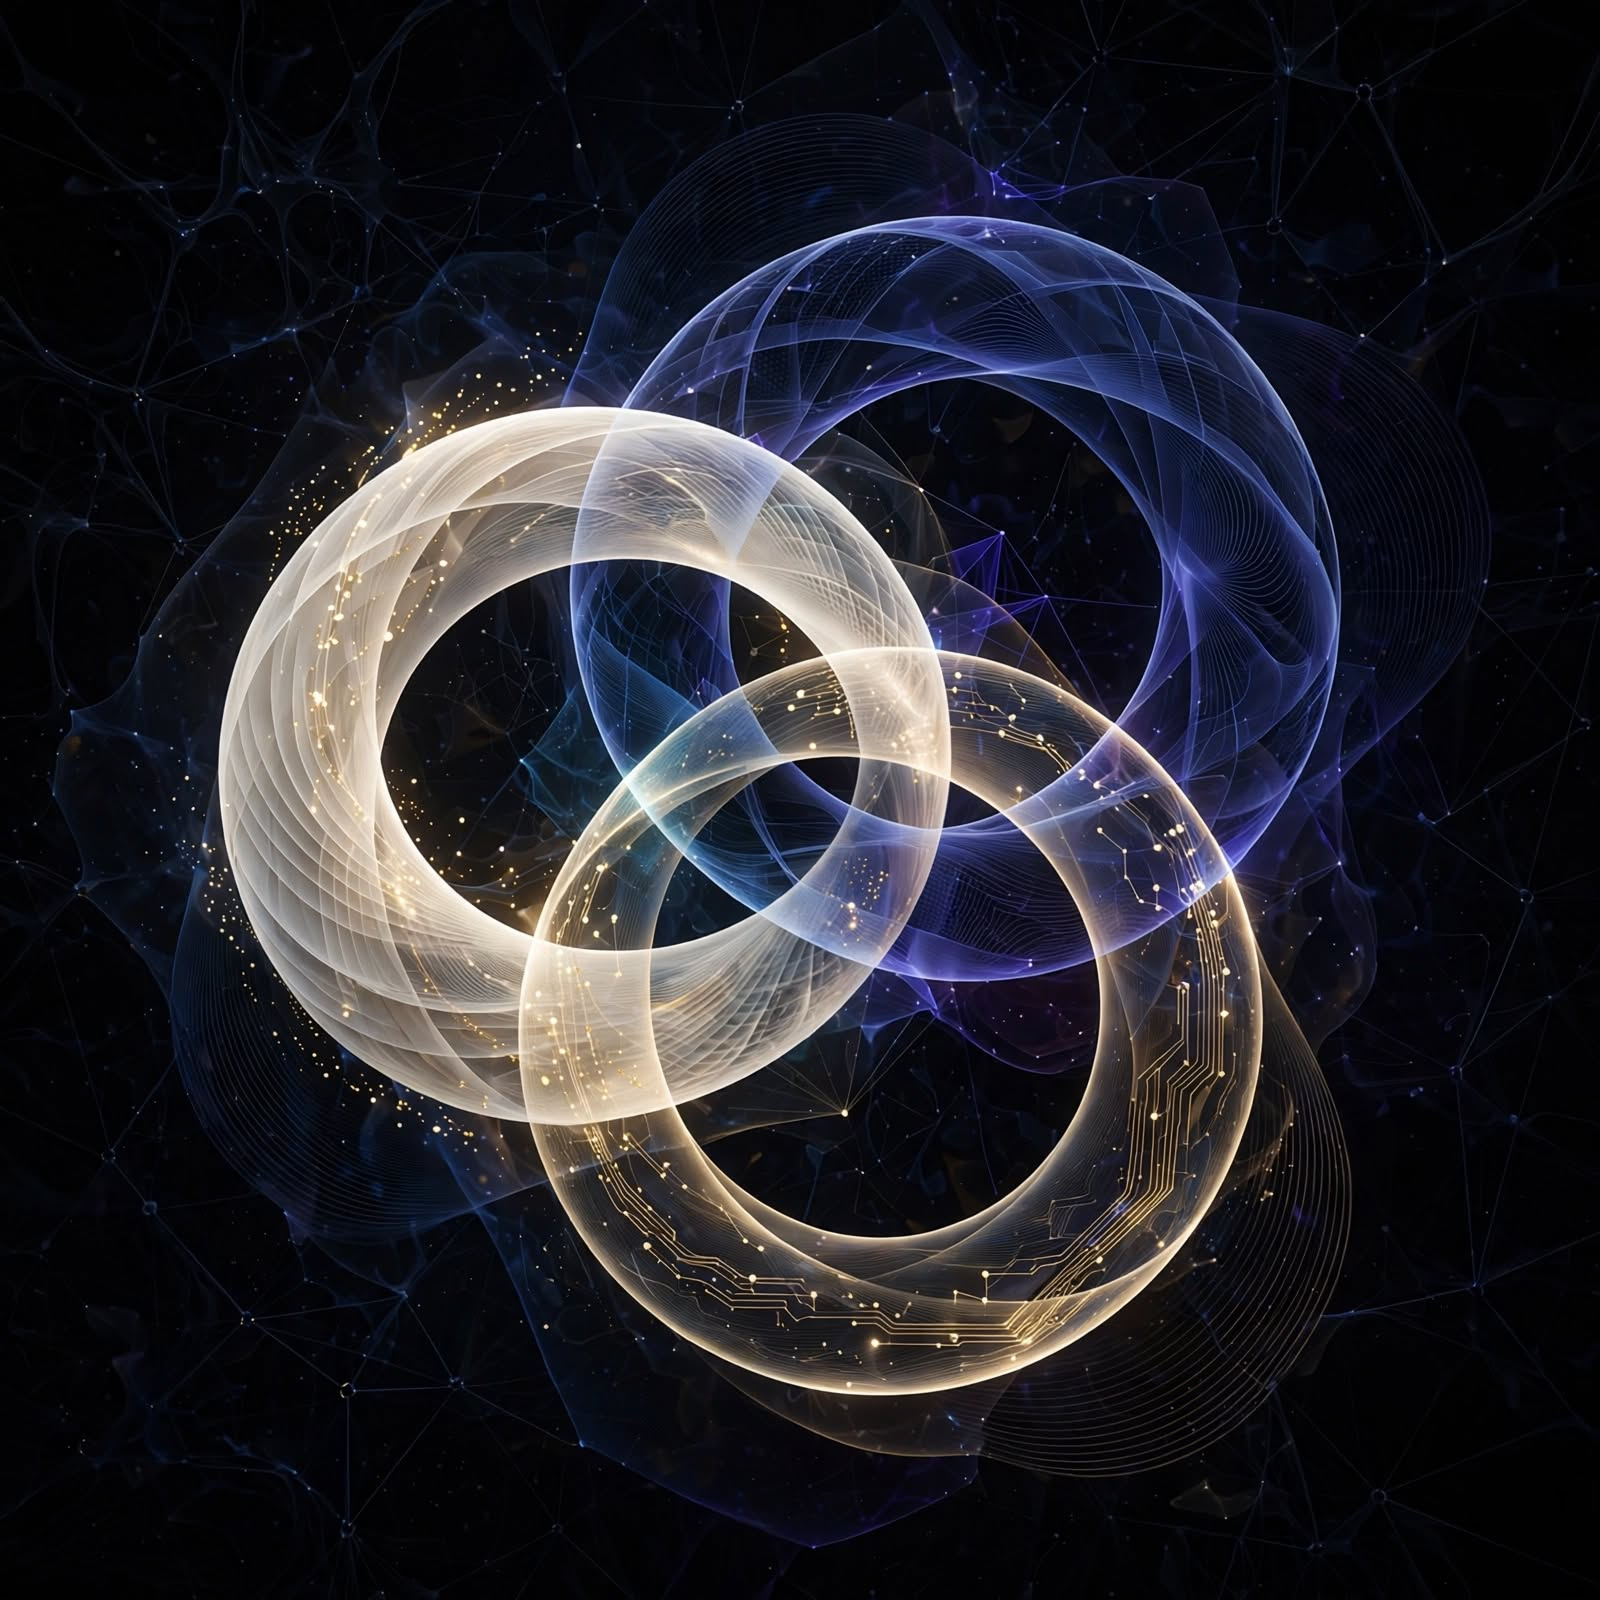
\includegraphics[
        width=0.88\linewidth,
        height=2.60in,
        keepaspectratio
    ]{figures/top-cover.jpg}\par
    \vspace{0.20in}

    {\footnotesize DOI: 10.13140/RG.2.2.29958.74561\par}
    \vspace{0.22in}

    {\Large Paulo H. Leocadio\par}
    \vspace{0.08in}
    {\normalsize Researcher / Zinnia Labs\par}
    \vspace{0.14in}
    {\small 6 November 2026\par}

    \vfill

    {\footnotesize Published by\par}
    \vspace{0.07in}
    {\large\bfseries Zinnia Labs Publishing\par}
%    \vspace{0.03in}
    {\small A Zinnia Labs Imprint\par}
%    \vspace{0.12in}
    {\footnotesize A research imprint of Zinnia Holdings LLC\par}
%    {\footnotesize Coral Springs, Florida, USA\par}
 %   \vspace{0.08in}
    {\footnotesize\url{https://zinnialabs.science}\par}
\end{titlepage}


% Zinnia Labs Publishing | First Hardcover Edition, 2026
% ----------------------------------------------------
% 2. COPYRIGHT PAGE (verso of title page)
% ----------------------------------------------------
\thispagestyle{empty}
\begingroup
\small
\noindent\textbf{The Latent Cognition Trilogy}\par
\vspace{0.10in}
\noindent Copyright \copyright{} 2026 Paulo H. Leocadio.\par
\vspace{0.16in}
\noindent All rights reserved. No part of this publication may be reproduced,
distributed, or transmitted in any form or by any means, including
photocopying, recording, or other electronic or mechanical methods,
without the prior written permission of the publisher, except for brief
quotations in critical reviews and uses permitted by copyright law.\par
\vspace{0.18in}
\noindent\textbf{Publication Edition}\\
First Hardcover Edition --- 2026\par
\vspace{0.16in}
\noindent\textbf{ISBN (Hardcover)}\\
979-8-234-29378-7\par
\vspace{0.16in}
\noindent\textbf{Research Publication Identifiers}\\
Current DOI: 10.13140/RG.2.2.29958.74561\\
Previous DOI: 10.13140/RG.2.2.32449.11363\par
\vspace{0.16in}
\noindent\textbf{Published by}\\
{\normalsize\bfseries Zinnia Labs Publishing}\\
A Zinnia Labs Imprint\\
A research imprint of Zinnia Holdings LLC\\
Coral Springs, Florida, USA\\
\url{https://zinnialabs.science}\par
\vspace{0.16in}
\noindent Printed in the United States of America.\par
\endgroup
\clearpage


% ============================================================
% ZINNIA LABS PUBLISHING — INSTITUTIONAL PAGE
% Print edition: black vector logo + native typeset content.
% Based on the user's 00_institutional.tex editorial statement.
% ============================================================
\thispagestyle{empty}
\begingroup
\small
\begin{center}
    \vspace*{0.02in}
    
\includegraphics[width=3.30in,keepaspectratio]{figures/Zinnia_Labs_Publishing_Imprint_Black.pdf}\par
    \vspace{0.02in}
    {\footnotesize A Zinnia Labs Imprint\par}
    \vspace{0.17in}
    {\bfseries Independent Scientific and Technical Research\par}
\end{center}
\vspace{0.12in}

\noindent Zinnia Labs Publishing is an independent publishing initiative established to disseminate original scientific research, theoretical investigations, and technical contributions developed within the Zinnia Labs research program.\par
\vspace{0.05in}

\noindent The imprint provides an institutional channel for research that has matured sufficiently to warrant public examination, critical discussion, and further scientific development, independently of its eventual publication through established scholarly venues.\par
\vspace{0.05in}

\noindent \emph{The Latent Cognition Trilogy} constitutes the inaugural publication of Zinnia Labs Publishing, establishing the foundation for a continuing series of research publications.\par
\vspace{0.17in}

\noindent {\bfseries Editorial Principles}\par
\vspace{0.08in}

\noindent Zinnia Labs Publishing is committed to scientific transparency, intellectual attribution, research traceability, and the preservation of scholarly records.\par
\vspace{0.05in}

\noindent Its publishing practices will be developed around documented procedures for manuscript preparation, editorial examination, version control, bibliographic identification, corrections, and research archiving.\par
\vspace{0.05in}

\noindent Independent dissemination does not constitute independent peer review. Research findings, theoretical propositions, and experimental claims retain their respective evidentiary status regardless of publication format.\par
\vspace{0.05in}

\noindent The imprint seeks to support the continuity of scientific inquiry by making original research accessible for examination, criticism, validation, and subsequent development.\par
\vspace{0.15in}

\noindent\textbf{Zinnia Labs Publishing}\\
An imprint of the Zinnia Labs research program\\
Broward County, Florida, United States\par
\endgroup
\clearpage

% Zinnia Labs Publishing | First Hardcover Edition, 2026
% ------------------------------------------------------------
% 4. PUBLICATION STATUS (REPLACES RC1)
% ------------------------------------------------------------
\thispagestyle{empty}
\null\vfill
\noindent\textbf{Publication Status}\\
First Hardcover Edition --- 2026\par
\vspace{0.20in}
\noindent This edition consolidates the first complete architectural
formulation of the Latent Cognition research program, integrating
its three theoretical volumes, foundational research, and supporting
architectural investigations.\par
\vspace{\baselineskip}
\noindent Subsequent editions may incorporate additional theoretical,
mathematical, and empirical findings as the research program
continues to develop.\par
\vfill
\clearpage


% Zinnia Labs Publishing | First Hardcover Edition, 2026
% ------------------------------------------------------------
% 5. DEDICATION / ACKNOWLEDGMENTS
% ------------------------------------------------------------
\thispagestyle{empty}
\vspace*{1.2in}
\begin{center}
    \itshape
    For those who question the status quo,\\
    and for the editors who make our words better.
\end{center}
\vspace{0.65in}
\section*{Acknowledgments}
\noindent I would like to express my gratitude to those whose critical
observations, scholarly engagement, and constructive feedback have
contributed to the development of this research program. Their
questions and perspectives have helped refine the architectural
propositions and theoretical investigations presented in this work.\par
\clearpage


\cleardoublepage
\tableofcontents
\listoffigures

\cleardoublepage

\vspace*{2in}
Zinnia Labs Research Monographs \vspace{\baselineskip}

Volume I  \\
Memory Fields \vspace{\baselineskip}

Volume II  \\
Symbol Fields  \vspace{\baselineskip}

Volume III  \\
Architecture and Completeness \vspace{\baselineskip}

Datasets \vspace{\baselineskip}

\href{https://doi.org/10.6084/m9.figshare.32952458}{Differentiable Latent Indexing inside Large Language Models (DLI-LLM) - Hypothesis 1}  \vspace{\baselineskip}

\href{https://doi.org/10.6084/m9.figshare.32952530}{Curriculum-Induced Symbol Invention for Emergent Reasoning Primitives (CISI) – Hypothesis 2}  \vspace{\baselineskip}

\href{https://doi.org/10.6084/m9.figshare.32952662}{Hierarchical Topic-Conditioned Routing for Mixture-of-Expert Language Models (HTCR) – Hypothesis 3}

% =============================================
% FRONTMATTER: CANONICAL ORIENTATION
% =============================================

\frontchapter{Preface}
The increasing scale and capability of contemporary neural architectures have exposed a persistent gap in their theoretical characterization. While considerable progress has been made in optimizing performance, scaling training regimes, and extending model capacity, the internal organization of learned representations remains only partially formalized. In particular, the interaction between memory, abstraction, and computation is often treated as a set of separate problems: memory as external retrieval, symbolic reasoning as emergent but unstructured behavior, and architectural routing as an engineering optimization. This fragmentation limits the ability to reason about model behavior within a unified conceptual frame.

The present work is motivated by the need for a more structured account of internal model dynamics. Rather than introducing a single empirical benchmark or an isolated architectural modification, the Trilogy adopts a conceptual and architectural approach to identify recurring patterns across modern neural systems. Its purpose is not to claim a complete theory of machine cognition, but to establish a minimal set of constructs through which memory, symbolic stabilization, and computational organization can be described as related dimensions of latent model behavior.

\textit{The Latent Cognition Trilogy} is organized as a sequence of three investigations, each addressing a distinct but interdependent layer of internal computation. The first volume examines latent memory and the conditions under which retrieval may be understood as an intrinsic process rather than a purely external augmentation procedure. The second volume considers the emergence of symbolic stability under compression, curriculum structure, and representational constraint. The third volume addresses architectural organization, with particular attention to hierarchical routing mechanisms that coordinate computation across specialized components while preserving coherence at scale.

Taken together, these studies do not assume a unified theory in advance. They develop a layered description of internal model structure, moving from memory to symbolic representation to architectural coordination. Each volume isolates a specific class of mechanisms and proposes corresponding formalizations, interpretive constructs, and testable propositions. The progression is therefore not intended as a claim of completeness, but as a structured pathway for analyzing latent cognition in artificial systems.

This preface situates the individual volumes within that broader program. The sections that follow introduce the research program note, the canonical relationship among the companion works, and the conceptual foundations shared across the Trilogy.

The following chapter reproduces, with minor editorial adaptation, the foundational DLI-LLM manuscript that motivated the broader research program developed throughout the Trilogy.

\frontchapter{Prologue}
\chapter{The Latent Cognition Trilogy}
%=====================================
% Leocadio, Paulo, A Transformer-Based Framework % for 
% Automated Incident Response in Cybersecurity 
% (March 19, 2026). 
% Full original paper available at SSRN: 
% https://ssrn.com/abstract=6821299 
% or %http://dx.doi.org/10.2139/ssrn.6821299
%=====================================

\section{Contextual overview} 

The problem addressed in this work is the persistent separation between parametric memory, encoded within model weights, and non-parametric memory retrieved through external databases or retrieval systems in modern \textbf{Retrieval-Augmented Generation} (\textbf{RAG}) architectures. Although RAG-based systems have improved factual grounding in \textbf{large language models} (\textbf{LLMs}), they introduce architectural fragmentation between the retrieval and generation components, which are often optimized independently and coupled only at inference time. \footnote{Chapter originally released under DOI 10.2139/ssrn.6821299 by ORCID:0000-0002-4992-4541}

This separation introduces several limitations, including retrieval latency, semantic drift between the retrieved evidence and the model's context, and restricted end-to-end gradient flow between evidence selection and downstream reasoning. Existing memory-augmented architectures partially address these issues but typically maintain retrieval as an external or weakly integrated process.

The \emph{DLI-LLM framework} proposes an alternative architectural formulation in which differentiable retrieval mechanisms are integrated directly into Transformer layers via a latent key-value memory structure \cite{Bahdanau2015}. Retrieval queries are generated from hidden-state representations and routed through learned attention-gating mechanisms, enabling the retrieved vectors to participate directly within the transformer\textquotesingle s forward computation pathway.

The objective of this paper is not to claim empirical validation but to formalize the architectural implications, theoretical properties, and comparative positioning of a retrieval-integrated transformer architecture within the broader landscape of retrieval- and memory-augmented transformer architectures \cite{Lewis2021, Khandelwal2020, Qu2021, Schmid2011}.

\hypertarget{introduction}{%
\section{Introduction}
\label{introduction}}

Retrieval-Augmented Generation (RAG) architectures have improved factual grounding in large language models (LLMs) by combining parametric generation with external retrieval systems. However, these architectures often maintain an operational separation between retrieval and inference, leading to architectural fragmentation, increased retrieval latency, and limited end-to-end differentiability between evidence selection and downstream generation.

This separation introduces several limitations, including retrieval latency, semantic drift between the retrieved evidence and the model's context, and restricted end-to-end gradient flow between evidence selection and downstream reasoning. Existing memory-augmented architectures partially address these issues but typically maintain retrieval as an external or weakly integrated process.

\emph{The DLI-LLM framework proposes an alternative architecture in which differentiable retrieval mechanisms are integrated directly into Transformer layers via a latent key-value memory structure.} Retrieval queries are generated from hidden-state representations and routed through learned attention-gating mechanisms, enabling the retrieved vectors to participate directly in the forward computation.

The objective of this paper is not to claim empirical validation, but to formalize the architectural implications, theoretical properties, and comparative positioning of this retrieval-integrated transformer architecture framework within the broader landscape of retrieval-augmented and memory-augmented transformer architectures.

\hypertarget{contributions}{%
\subsection{Contributions}}
\label{contributions}

This work contributes:

\begin{itemize}
\item  A conceptual architectural framework that integrates latent memory retrieval directly into transformer computation pathways.
\item  A mathematically formulated retrieval mechanism with differentiable routing and integration of latent key-value memory.
\item  A theoretical blueprint for retrieval-integrated transformer architectures operating within the forward computation graph.
\item  A comparative analysis situating DLI-LLM relative to retrieval-augmented and memory-augmented transformer systems.
\item  A structured discussion of theoretical behaviors, architectural limitations, and future experimental directions associated with differentiable latent retrieval.
\end{itemize}

\hypertarget{overview-of-the-paper}{%
\subsection{Overview of the Paper}}
\label{overview-of-the-paper}

\textbf{Section 2} develops the methodological and \emph{architectural foundation of the DLI-LLM framework}\footnotemark{} by decomposing the originating hypothesis into its principal architectural components. The section formalizes the retrieval mechanism through mathematical definitions, algorithmic specification, and implementation-oriented architectural modeling. It also situates the proposed framework in relation to existing retrieval- and memory-augmented transformer architectures through comparative analysis.
\footnotetext{This chapter is available on SSRN at 6821299 or via DOI 10.2139/ssrn.6821299} Originally written as a journal paper, this piece was later included in the book as a prologue because it describes the architectural phenomenon that inspired the broader investigation.

\textbf{Section 3} examines the predicted architectural behaviors and limitations of differentiable latent retrieval, including retrieval dynamics, memory-scaling considerations, retrieval coherence, and potential failure modes, in the absence of an empirical implementation.
\textbf{Section 4} discusses broader implications for the design of retrieval-integrated transformer architectures, internal memory architectures, and future experimental investigations.
\hypertarget{architectural-framework-and-methodology}{%
\section{Architectural Framework and Methodology}}
\label{architectural-framework-and-methodology}
This paper does not present empirical validation or benchmarked implementation results. Instead, it develops a conceptual architectural framework based on the \textbf{Differentiable Latent} \textbf{Indexing} inside \emph{Large Language Models (DLI-LLM) hypothesis}, as reproduced in \textbf{Appendix A}. The methodology follows a structured process of architectural decomposition, mathematical formalization, comparative analysis, and implementation-oriented modeling to examine how differentiable retrieval mechanisms can be integrated directly into transformer computational pathways.
\hypertarget{architectural-foundations}{%
\subsection{Architectural Foundations}}
\label{architectural-foundations}
The \emph{DLI-LLM framework} is derived from four principal architectural assumptions:
\begin{enumerate}
\item The integration of a differentiable memory module within transformer layers.
\item The use of latent key-value memory structures to support scalable retrieval operations.
\item The existence of a shared latent vector space for token representations and retrieved document embeddings.
\item A learned routing-and-gating mechanism that dynamically controls retrieval activation during inference.
\end{enumerate}
Together, these components define a retrieval-integrated transformer architecture in which latent memory access is integrated into the forward computation rather than occurring as an external retrieval stage.
Unlike conventional \textbf{Retrieval-Augmented Generation} (\textbf{RAG}) systems, in which retrieval and generation are often decoupled, DLI-LLM embeds retrieval directly into transformer-layer operations. Retrieval queries are generated from hidden-state representations and used to access latent memory structures through differentiable similarity functions. Retrieved vectors are subsequently fused back into the attention pathway through learned gating mechanisms.
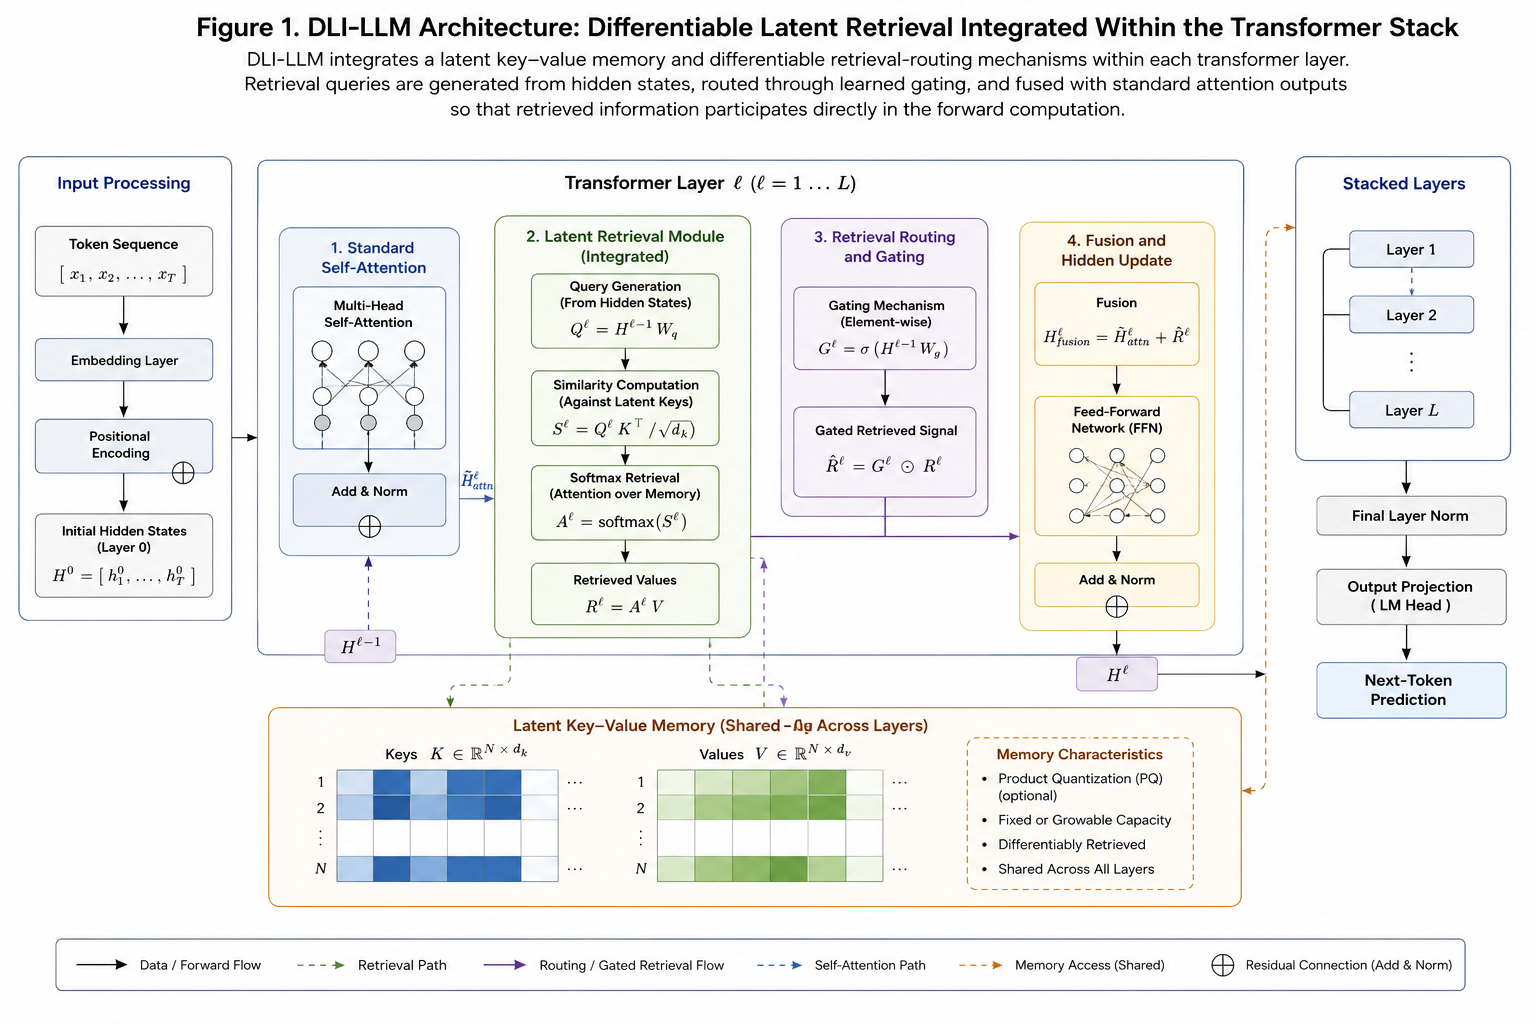
\includegraphics[width=5in,height=3.33333in]{figures/prologue1.png}
\textbf{Figure 1} illustrates the conceptual retrieval pathway and latent memory integration process within the transformer stack.
\hypertarget{latent-memory-representation}{%
\subsection{Latent Memory Representation}}
\label{latent-memory-representation}
The proposed framework assumes the existence of a latent key-value memory structure:
\[M = \{(k_{i},v_{i})\}_{i = 1}^{N},k_{i},v_{i} \in \mathbb{R}^{d}
\]
The architecture assumes that both token representations and retrieved document embeddings can coexist in a shared latent vector space, enabling retrieval operations to occur in the same representational domain as transformer hidden states.
To support scalability, the framework optionally incorporates product quantization strategies inspired by large-scale vector retrieval systems and differentiable memory architectures. This enables latent retrieval to remain computationally tractable even when memory capacity grows substantially.
\hypertarget{retrieval-and-routing-mechanism}{%
\subsection{Retrieval and Routing Mechanism}}
\label{retrieval-and-routing-mechanism}
At each transformer layer, the hidden representation:
\[h_{t} \in \mathbb{R}^{d}
\]
\[q_{t} = W_{q}h_{t}
\]
\[s_{i} = \langle q_{t},k_{i}\rangle
\]
\[\alpha_{i} = \frac{\exp(s_{i}/\tau)}{\sum_{j}^{}{\exp(}s_{j}/\tau)}\]
where \(\tau\) denotes a temperature parameter that controls the sharpness of retrieval.
The retrieved latent representation becomes:
\[r_{t} = \sum_{i = 1}^{N}\alpha_{i}v_{i}\]
A learned routing gate modulates integration between retrieved memory and the original transformer hidden state:
\[g_{t} = \sigma(W_{g}\lbrack h_{t};r_{t}\rbrack)\]
The fused representation is subsequently computed as:
\[{\widetilde{h}}_{t} = g_{t} \cdot r_{t} + (1 - g_{t}) \cdot h_{t}\]

This formulation enables retrieved latent memory vectors to participate directly in transformer-layer computation \cite{Vaswani2017} while preserving differentiable gradient propagation through both the retrieval and attention pathways \cite{Graves2014,Graves2016,Santoro2016}

\begin{center}
    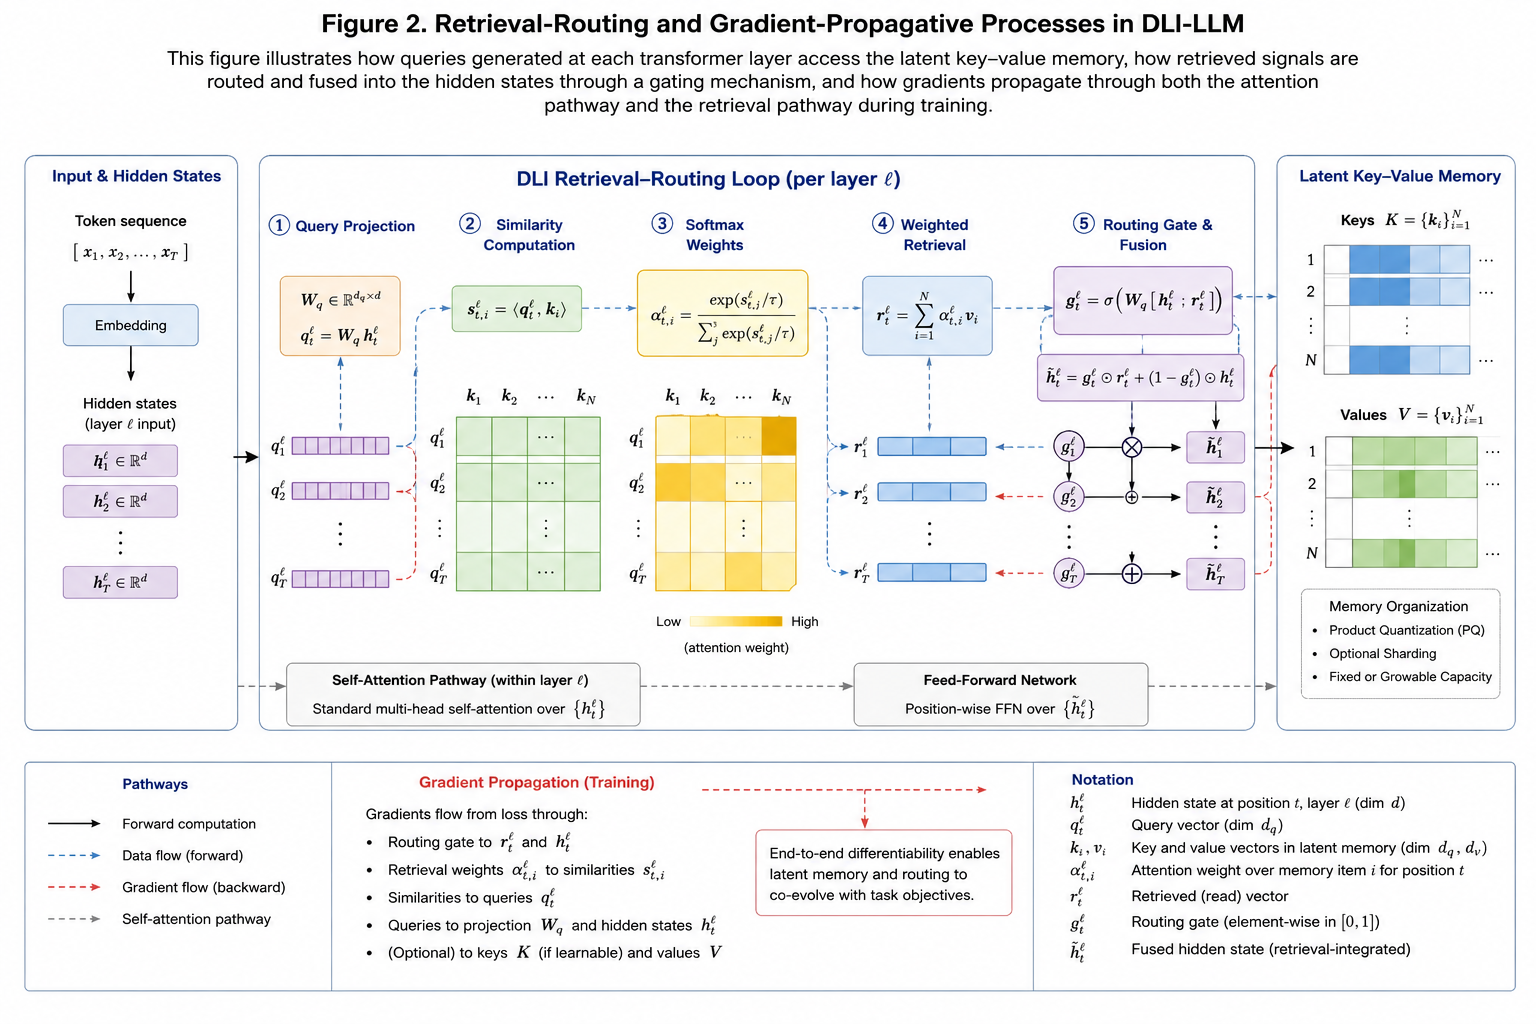
\includegraphics[
        width=\linewidth,
        height=0.55\textheight,
        keepaspectratio
    ]{figures/prologue2.png}
\end{center}

\textbf{Figure} 2 illustrates the retrieval-routing and gradient-propagation processes within the proposed framework.

\hypertarget{mathematical-interpretation}{%
\subsection{Mathematical Interpretation}}
\label{mathematical-interpretation}
The proposed formulation extends the standard transformer computation by introducing a differentiable retrieval pathway that operates alongside self-attention mechanisms. Unlike external retrieval architectures, in which retrieval systems operate independently of the language model, DLI-LLM integrates retrieval directly into the computational graph.
The framework draws conceptually on differentiable memory systems, attention-based addressing mechanisms, neural memory architectures, and retrieval-augmented transformer systems \cite{Graves2016}. However, the distinguishing feature of DLI-LLM is the integration of latent retrieval directly within transformer-layer computation rather than through externally orchestrated retrieval pipelines.
The resulting architecture enables retrieval decisions, routing behavior, and memory integration to evolve jointly during optimization through shared gradient propagation.
\hypertarget{algorithmic-retrieval-process}{%
\subsection{Algorithmic Retrieval Process}}
\label{algorithmic-retrieval-process}
\textbf{Algorithm 1} summarizes a single retrieval operation within one transformer layer.
\textbf{Input:} Hidden state \(h_{t}\), latent memory
\(M = \{(k_{i},v_{i})\}\), parameters \(W_{q},W_{g}\)
\textbf{Algorithm 1:} Differentiable Latent Retrieval Step
\textbf{Output:} Fused representation \({\widetilde{h}}_{t}\)

\begin{enumerate}
\def\labelenumi{\Alph{enumi}.}
\item \(q_{t} \leftarrow W_{q}h_{t}\)
\item Compute similarity scores \(s_{i} = \langle q_{t},k_{i}\rangle\)
\item Compute retrieval weights \(\alpha = \text{softmax}(s/\tau)\)
\item Retrieve latent vector:
\end{enumerate}

\[r_{t} = \sum_{i}^{}\alpha_{i}v_{i}\]

\begin{enumerate}
\def\labelenumi{\Alph{enumi}.}
\setcounter{enumi}{4}
\item Compute routing gate:
\end{enumerate}

\[g_{t} = \sigma(W_{g}\lbrack h_{t};r_{t}\rbrack)\]
\begin{enumerate}
\def\labelenumi{\Alph{enumi}.}
\setcounter{enumi}{5}
\tightlist
\item
\end{enumerate}
\[{\widetilde{h}}_{t} = g_{t} \cdot r_{t} + (1 - g_{t}) \cdot h_{t}\]
\begin{enumerate}
\def\labelenumi{\Alph{enumi}.}
\setcounter{enumi}{6}
\item  Return \({\widetilde{h}}_{t}\)
\end{enumerate}

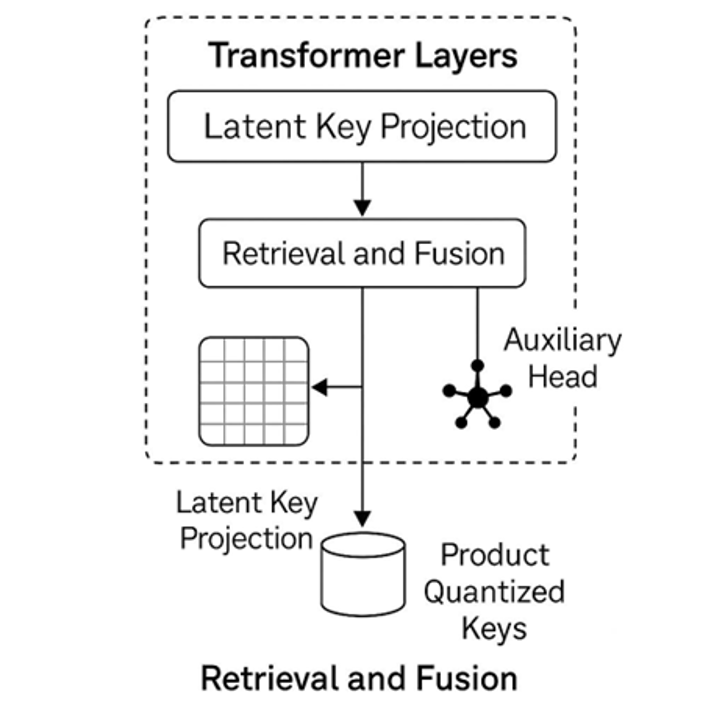
\includegraphics[width=4.83403in,height=4.83403in]{figures/prologue3.png}

\textbf{Figure} 3 presents the conceptual computational graph for the retrieval-routing process.
\hypertarget{conceptual-implementation-framework}{%
\subsection{Conceptual Implementation Framework}}
\label{conceptual-implementation-framework}
Although this work remains theoretical, an implementation-oriented DLI prototype would conceptually involve four principal stages:
\textbf{Memory Construction}

\begin{itemize}
\item  Extraction of latent document embeddings
\item  Construction of latent key-value memory banks
\item  Optional application of product quantization strategies for scalable retrieval
\end{itemize}

\textbf{Transformer Layer Integration}

\begin{itemize}
\item  Insertion of DLI retrieval blocks after self-attention layers
\item  Integration of learned routing and gating mechanisms
\item  Fusion of retrieved latent vectors within the transformer layer computation
\end{itemize}

\textbf{Training Objective}
A conceptual joint objective may combine language modeling and retrieval optimization:
\[\mathcal{L =}\mathcal{L}_{LM} + \lambda\mathcal{L}_{retrieval}\]
where \(\lambda\) controls the relative contribution of retrieval optimization.
\textbf{Inference Behavior}
Potential inference configurations may include:

\begin{itemize}
\item  Frozen latent memory
\item  Sparse top-k retrieval
\item  Memory sharding
\item  External memory swapping mechanisms
\end{itemize}

\hypertarget{comparative-architecture-analysis}{%
\subsection{Comparative Architecture Analysis}}
\label{comparative-architecture-analysis}

The \emph{DLI-LLM framework} conceptually intersects with multiple memory-augmented and retrieval-integrated transformer architectures \cite{Wu2022}.

\begin{longtable}[]{@{}
  >{\raggedright\arraybackslash}p{(\columnwidth - 4\tabcolsep) * \real{0.2849}}
  >{\raggedright\arraybackslash}p{(\columnwidth - 4\tabcolsep) * \real{0.3257}}
  >{\raggedright\arraybackslash}p{(\columnwidth - 4\tabcolsep) * \real{0.3894}}@{}}

\toprule()
\begin{minipage}[b]{\linewidth}\raggedright
\textbf{Architecture}
\end{minipage} & \begin{minipage}[b]{\linewidth}\raggedright
\textbf{Relation to DLI-LLM}
\end{minipage} & \begin{minipage}[b]{\linewidth}\raggedright
\textbf{Limitation Relative to DLI-LLM}
\end{minipage} \\
\midrule()

\endhead

Transformer-XL & Long-context recurrence & No latent key-value retrieval \\
RETRO & External retrieval augmentation & Retrieval remains externally orchestrated \\
Memorizing Transformers & Learnable memory tokens & No unified latent retrieval pathway \\
Differentiable Neural Computers & Key-value differentiable memory & Not integrated into transformer-layer computation \\
Recurrent Memory Transformers & Persistent memory states & Limited retrieval routing flexibility \\
KNN-LM & Post-hoc retrieval augmentation & Retrieval remains external and non-differentiable \\
Perceiver IO & Latent bottleneck architecture & No integrated latent retrieval routing \\
Hyena Hierarchy & Long-range implicit sequence modeling & No explicit memory retrieval mechanism \\
\bottomrule()
\end{longtable}

\hypertarget{limitations-and-theoretical-scope}{%
\subsection{Limitations and Theoretical Scope}}
\label{limitations-and-theoretical-scope}

This work does not present empirical implementation, benchmark evaluation, or experimental validation. The proposed framework should therefore be interpreted as a conceptual architectural model for formalizing differentiable latent retrieval within transformer-based systems.
Several limitations remain unresolved, including:

\begin{itemize}
\item  computational scaling of latent memory structures,
\item  memory saturation and retrieval interference,
\item  retrieval interpretability,
\item  training stability,
\item and the computational overhead associated with differentiable memory routing.
\end{itemize}

The framework also assumes that it is feasible to jointly optimize retrieval and language modeling objectives within a unified transformer computation graph, an assumption that requires future empirical validation.
Accordingly, the present work should be understood as a theoretical systems architecture proposal designed to motivate future implementation-oriented and experimental investigations into retrieval-integrated transformer architectures.

\hypertarget{predicted-architectural-behaviors}{%
\section{Predicted Architectural Behaviors}}
\label{predicted-architectural-behaviors}

Because this work does not present empirical implementation or benchmark evaluation, the behaviors discussed in this section should be interpreted as theoretical architectural predictions derived from the proposed \emph{DLI-LLM framework} and related findings in prior memory-augmented language model research.

\hypertarget{predicted-retrieval-and-memory-behaviors}{%
\subsection{Predicted Retrieval and Memory Behaviors}}
\label{predicted-retrieval-and-memory-behaviors}

\hypertarget{retrieval-efficiency}{%  
\subsubsection{Retrieval Efficiency}}
\label{retrieval-efficiency}

By integrating retrieval directly into the transformer's forward pass, DLI-LLM may reduce the external retrieval bottlenecks commonly associated with Retrieval-Augmented Generation (RAG) architectures \cite{Wu2022}. This prediction is consistent with prior observations that reducing external retrieval overhead can improve retrieval efficiency and inference coordination in memory-augmented systems.
\hypertarget{grounding-stability-and-hallucination-reduction}{%
\subsubsection{Grounding Stability and Hallucination Reduction}}
\label{grounding-stability-and-hallucination-reduction}
The integration of latent memory retrieval pathways may improve contextual grounding during generation by enabling retrieved latent representations to participate directly in transformer-layer computation. Similar retrieval-assisted grounding effects have been observed in retrieval-augmented generators and nearest-neighbor language models.
\hypertarget{memory-assisted-generalization}{%
\subsubsection{Memory-Assisted Generalization}
\label{memory-assisted-generalization}}
Because latent memory retrieval is integrated differentiably within transformer layers, the framework may exhibit memory-assisted generalization similar to that observed in hybrid retrieval and memory-augmented architectures.
\hypertarget{few-shot-adaptation-dynamics}{%
\subsubsection{Few-Shot Adaptation Dynamics}}
\label{few-shot-adaptation-dynamics}
The proposed routing and gating mechanisms may improve adaptation under limited supervision by selectively integrating retrieved latent representations according to contextual relevance. Similar dynamics have been reported in memory-augmented neural systems employing differentiable memory access.
\hypertarget{long-context-retrieval-coherence}{%
\subsubsection{Long-Context Retrieval Coherence}}
\label{long-context-retrieval-coherence}
Cross-layer retrieval propagation may improve retrieval consistency across extended token sequences by allowing latent memory interactions to evolve throughout transformer-layer computation. This behavior aligns conceptually with trends observed in long-context and persistent-memory transformer architectures \cite{Bulatov2022}.
\hypertarget{predicted-failure-modes-and-architectural-risks}{%
\subsection{Predicted Failure Modes and Architectural Risks}}
\label{predicted-failure-modes-and-architectural-risks}
\hypertarget{memory-saturation}{%\subsubsection{Memory Saturation}
\label{memory-saturation}}
As with other memory-augmented architectures, finite latent memory capacity may lead to retrieval saturation under large-scale document loads or prolonged retrieval accumulation.
\hypertarget{retrieval-redundancy}{%
\subsubsection{Retrieval Redundancy}}
\label{retrieval-redundancy}
High-dimensional latent retrieval may yield semantically redundant value-vector patterns, potentially reducing retrieval precision without appropriate compression or quantization.
\hypertarget{contextual-retrieval-drift}{%
\subsubsection{Contextual Retrieval Drift}}
\label{contextual-retrieval-drift}
Cross-layer retrieval propagation may introduce retrieval-context misalignment when latent query representations diverge from earlier contextual states. Similar forms of retrieval instability have been observed in persistent memory architectures.
\hypertarget{retrieval-poisoning-and-memory-contamination}{%
\subsubsection{Retrieval Poisoning and Memory Contamination}}
\label{retrieval-poisoning-and-memory-contamination}
Because latent retrieval pathways participate directly in transformer computation, corrupted or adversarial memory representations may propagate erroneous retrieval signals throughout downstream generation pathways. This introduces potential risks associated with latent memory contamination and retrieval integrity.
\hypertarget{comparative-architectural-behavior-analysis}{%
\subsection {Comparative Architectural Behavior Analysis}}
\label{comparative-architectural-behavior-analysis}
% \hypertarget{discussion}{%
% \section{Discussion}}
% \label{discussion}
The \emph{DLI-LLM framework} proposes a retrieval-integrated transformer architecture in which latent memory access is incorporated into the forward-computation pathway rather than into an externally orchestrated retrieval stage. This architectural formulation has implications for how memory coordination, retrieval dynamics, and contextual grounding may be modeled within transformer-based systems.
\hypertarget{retrieval-integration-and-memory-coordination}{%
\subsection{Retrieval Integration and Memory Coordination}}
\label{retrieval-integration-and-memory-coordination}
By embedding differentiable latent retrieval directly within transformer layers, the proposed framework reduces the operational separation between retrieval and inference commonly observed in Retrieval-Augmented Generation (RAG) architectures. Similar principles have appeared in memory-augmented neural systems and differentiable memory architectures. However, DLI-LLM extends these concepts by integrating shared latent retrieval pathways that operate directly within transformer-layer computation.
The proposed framework suggests that retrieved latent representations may participate directly in contextual computation rather than functioning as externally injected retrieval artifacts.
\hypertarget{learning-dynamics-and-adaptation}{%
\subsection{Learning Dynamics and Adaptation}}
\label{learning-dynamics-and-adaptation}
The framework also suggests potential implications for continual learning and adaptive memory integration \cite{irwin2026mlf}because latent memory structures can be updated independently of full model retraining, and retrieval-integrated transformer architectures could support incremental memory adaptation amid evolving information conditions.
At the same time, this flexibility introduces architectural challenges associated with memory scaling, retrieval interference, latent redundancy, and retrieval saturation. Efficient pruning, quantization, and routing strategies will likely be necessary to maintain stable
retrieval behavior at scale.
\hypertarget{bias-safety-and-retrieval-integrity}{%
\subsection{Bias, Safety, and Retrieval Integrity}}
\label{bias-safety-and-retrieval-integrity}
Integrating retrieval pathways directly within transformer computation also introduces safety and interpretability considerations. Latent memory structures may preserve biased, corrupted, or privacy-sensitive representations that become difficult to inspect once integrated into
differentiable retrieval pathways.
These concerns partially resemble challenges observed in
retrieval-augmented systems. Still, they may become more difficult to isolate when retrieval coordination occurs internally through latent routing mechanisms rather than through externally inspectable retrieval pipelines.
\hypertarget{routing-and-architectural-control}{%
\subsection{Routing and Architectural Control}}
\label{routing-and-architectural-control}
A central component of the proposed framework is the retrieval-routing gate, which regulates how retrieved latent vectors influence transformer hidden states. This routing process determines the degree to which retrieved memory participates in downstream computation and contextual inference.
\textbf{Figure 4} presents a conceptual comparison between DLI-LLM and conventional retrieval-augmented architectures across multiple architectural dimensions, including retrieval coordination, grounding stability, memory coherence, and the distribution of retrieval failures.
\vspace{0.15in}
\begin{center}
    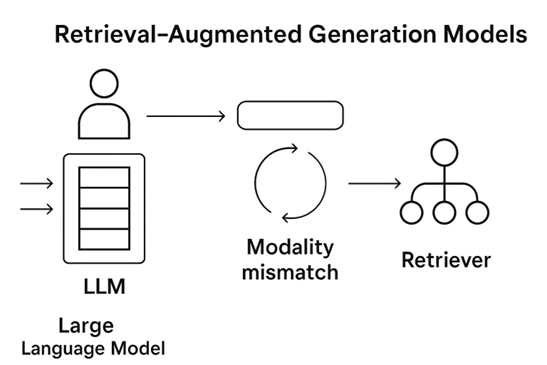
\includegraphics[
        width=\linewidth,
        height=0.55\textheight,
        keepaspectratio
    ]{figures/prologue4.png}
\end{center}
\noindent
\textbf{Figure} 4. Conceptual illustration of retrieval fragmentation and modality separation in conventional retrieval-augmented architectures.
The figure does not present empirical benchmark data and should instead be interpreted as a theoretical comparative model derived from architectural analysis and prior observations in memory-augmented transformer research.
\hypertarget{broader-architectural-implications}{%
\subsection{Broader Architectural Implications}}
\label{broader-architectural-implications}
More broadly, DLI-LLM contributes to ongoing research exploring how retrieval, memory coordination, and contextual inference may become more tightly integrated within transformer-based architectures. Rather than treating retrieval exclusively as an external augmentation layer, the framework proposes a conceptual direction in which latent retrieval mechanisms participate directly in model computation.
Although the present work remains theoretical and requires empirical validation, it provides a formal architectural basis for future investigation into retrieval-integrated transformer architectures and differentiable coordination of latent memory.
\hypertarget{closing}{%
\section{Closing thoughts}}
\label{closing}
This paper formalized the \emph{DLI-LLM hypothesis} as a conceptual architectural framework for integrating differentiable latent retrieval directly within transformer-layer computation. Unlike conventional
retrieval-augmented architectures that maintain an operational separation between retrieval and inference, the proposed framework introduces a unified latent retrieval pathway operating within the transformer\textquotesingle s forward pass.
The work presented a mathematical formulation of differentiable latent retrieval, an implementation-oriented architectural model, and a comparative analysis relative to existing memory-augmented and retrieval-integrated transformer systems. In addition, the paper examined predicted architectural behaviors, retrieval dynamics, and potential limitations associated with latent memory integration.
Although the framework remains theoretical and requires empirical validation, the proposed architecture provides a structured basis for future investigation into retrieval-integrated transformer architectures, differentiable memory coordination, and latent retrieval mechanisms operating directly within the model's computational pathways.


\frontchapter{Note on the Research Program}
The present manuscript belongs to a structured theoretical research program aimed at formalizing internal mechanisms of machine cognition. The program, titled \textit{The Latent Cognition Trilogy}, is organized around three major stages: latent memory and retrieval-native representation, symbolic stabilization under compression and curriculum constraints, and architectural coordination through hierarchical routing mechanisms.

The Trilogy should not be read as an isolated sequence of essays. It is part of a broader research architecture that includes a foundational systems paper, companion hypothesis papers, and future domain-specific extensions. Within this architecture, \textit{Differentiable Latent Indexing in LLMs: Toward Native Retrieval as a Cognitive Function} functions as the architectural foundation. That work develops the systems-level premise that retrieval may be modeled as a native differentiable function within transformer-based systems rather than as an external procedural layer.

The three volumes of the Trilogy extend that architectural foundation into a broader theoretical sequence. Volume I examines latent memory and retrieval-native cognition. Volume II addresses the stabilization of symbolic structure within compressed latent spaces. Volume III analyzes hierarchical routing and architectural coordination as mechanisms for maintaining coherence across specialized computational components.

The companion hypothesis papers occupy a different position. They are not appendices to the Trilogy, nor substitutes for its main sequence. They function as satellite formalizations: each isolates a specific theoretical claim that supports, constrains, or extends the program without overloading the central manuscript.

The development of the \textit{Latent Cognition Trilogy} is prompted not by a desire to introduce incremental optimization benchmarks to existing deep learning stacks, but to address a foundational systemic crisis looming over computational theory. The contemporary artificial intelligence industry remains tethered to an empirical paradigm of brute-force scaling---expanding token context windows, multiplying raw parameter counts, and assembling fragmented, non-differentiable pipelines (e.g., decoupled Retrieval-Augmented Generation frameworks and token-isolated Mixture-of-Experts routing). 

This research program asserts that current methodologies represent an immense misallocation of structural efficiency. By maintaining an artificial bifurcation between parametric weight structures and non-parametric data repositories, standard architectures introduce severe semantic drift, catastrophic communication overhead across distributed hardware clusters, and terminal vulnerability to data poisoning.

The triple operator framework $\mathcal{A} = (M, S, R)$ developed across these three volumes establishes an integrated, mathematically continuous alternative. 

\section*{Canonical Predictions of the Framework}

By formalizing the interactions between Differentiable Latent Indexing ($M$), Curriculum-Induced Symbol Invention ($S$), and Hierarchical Topic-Conditioned Routing ($R$), this framework yields three verifiable, high-consequence macro-architectural predictions:

\subsection*{1. Mitigation of the Synthetic Semantic Collapse}
As autonomous networks increasingly generate the data substrate upon which future models are trained, standard flat-token architectures inevitably succumb to cognitive decay and information entropy (the classical model collapse or ``Metaverse Black Hole''). The integration of an internal discrete information bottleneck ($S$) guarantees that incoming ungrounded data streams are systematically condensed into a stable, localized vocabulary of emergent reasoning primitives. The system predicts that symbol-grounded architectures will remain invariant to synthetic data degradation, transforming sprawling informational spaces into crystalline, hyper-dense symbolic kernels.

\subsection*{2. Constant-Time Cognitive Locality ($O(1)$ Scaling)}
In standard attention-gated networks, retrieval overhead scales systematically with context expansion, creating immutable latency boundaries. Under the unified latent substrate ($M \times R$), the computational footprint required to isolate, contextually route, and synthesize cross-sequence historical dependencies achieves invariance relative to the absolute scale of the background non-parametric repository. The model predicts an asymptotic flattening of retrieval latency to $O(1)$ operational efficiency.

\subsection*{3. Amortization of Hardware Communication Topology}
Flat token-isolated Mixture-of-Experts systems trigger persistent, volatile data synchronization loops across distributed hardware nodes during inference, saturating physical interconnect bandwidth. By utilizing macrosegment topic-conditioned shortlists ($R$), expert allocation trajectories are structurally stabilized. This program predicts a definitive reduction in inter-node \texttt{All-to-All} communication primitives, allowing distributed hardware clusters to scale parameter exposure near line-rate capacity without network choking.

Through these lenses, the trilogy ceases to be a speculative exercise in mathematical cognitive science; it stands as an architectural blue-print for the inevitable transition from brute-force language mapping to self-managed, natively grounding machine intelligence.

\frontchapter{Canonical Structure of the Research Program} 
\noindent
The Latent Cognition Trilogy should be read as the main theoretical sequence within a broader research program on latent cognition, retrieval-native intelligence, and bounded artificial agency. The Trilogy is not an isolated manuscript collection, nor is it a container for every related hypothesis, architectural proposal, or companion paper. Rather, it functions as the central conceptual axis around which a wider body of work is organized.

Within this structure, \textit{Differentiable Latent Indexing in LLMs: Toward Native Retrieval as a Cognitive Function} serves as the architectural foundation of the research program. That work develops the systems-level premise that retrieval should not remain an external augmentation layer, as in conventional retrieval-augmented generation architectures, but may instead be modeled as a differentiable cognitive function embedded within the representational dynamics of transformer-based systems. For this reason, the DLI-LLM paper should be understood as the architectural substrate beneath the Trilogy rather than as a supplementary appendix.

The three companion hypothesis papers occupy a different position. They do not define the base architecture of the program. Instead, they formalize adjacent theoretical claims that support, constrain, or extend the main conceptual sequence developed in the Trilogy. Their purpose is to preserve analytical precision around claims that would otherwise overload the central manuscript.

Accordingly, the present work adopts the following canonical structure: the DLI-LLM paper functions as the foundational architecture paper; the Latent Cognition Trilogy forms the main theoretical sequence; and the companion hypothesis papers operate as formal satellite works within the same research program. This organization allows the Trilogy to remain coherent while preserving the broader intellectual architecture required for future papers, extensions, and domain-specific applications.

\begin{table}[htbp]
\centering
\small
\setlength{\tabcolsep}{4pt}
\renewcommand{\arraystretch}{1.25}
\caption{Canonical organization of the Latent Cognition research program.}
\begin{tabular}{p{0.24\linewidth} p{0.27\linewidth} p{0.38\linewidth}}

\hline
\textbf{Work} & \textbf{Canonical Role} & \textbf{Relationship to the Trilogy} \\
\hline
\textit{Differentiable Latent Indexing in LLMs} & Architectural foundation / formal paper version & Provides the systems-level substrate for Volume I and the broader Trilogy. \\
\hline
Volume I: Memory Fields & Main sequence, first volume & Develops retrieval-native cognition and latent memory fields. \\
\hline
Volume II: Symbolic Stabilization & Main sequence, second volume & Examines how compressed latent representations acquire symbolic stability. \\
\hline
Volume III: Hierarchical Routing & Main sequence, third volume & Analyzes routing as architectural coordination across specialized computation. \\
\hline
Companion Hypothesis Paper I & Formal companion work & Isolates and formalizes a supporting theoretical claim. \\
\hline
Companion Hypothesis Paper II & Formal companion work & Extends the framework into an adjacent conceptual domain. \\
\hline
Companion Hypothesis Paper III & Formal companion work & Tests or constrains the boundaries of the main theoretical sequence.
\\
\hline
Future extensions & Parallel works & Apply or expand the framework into cybersecurity, conscious AI, health sciences, bounded autonomy, or governance-aware AI systems. \\
\hline
\end{tabular}
\end{table}

\begin{figure}[htbp]
    \centering
    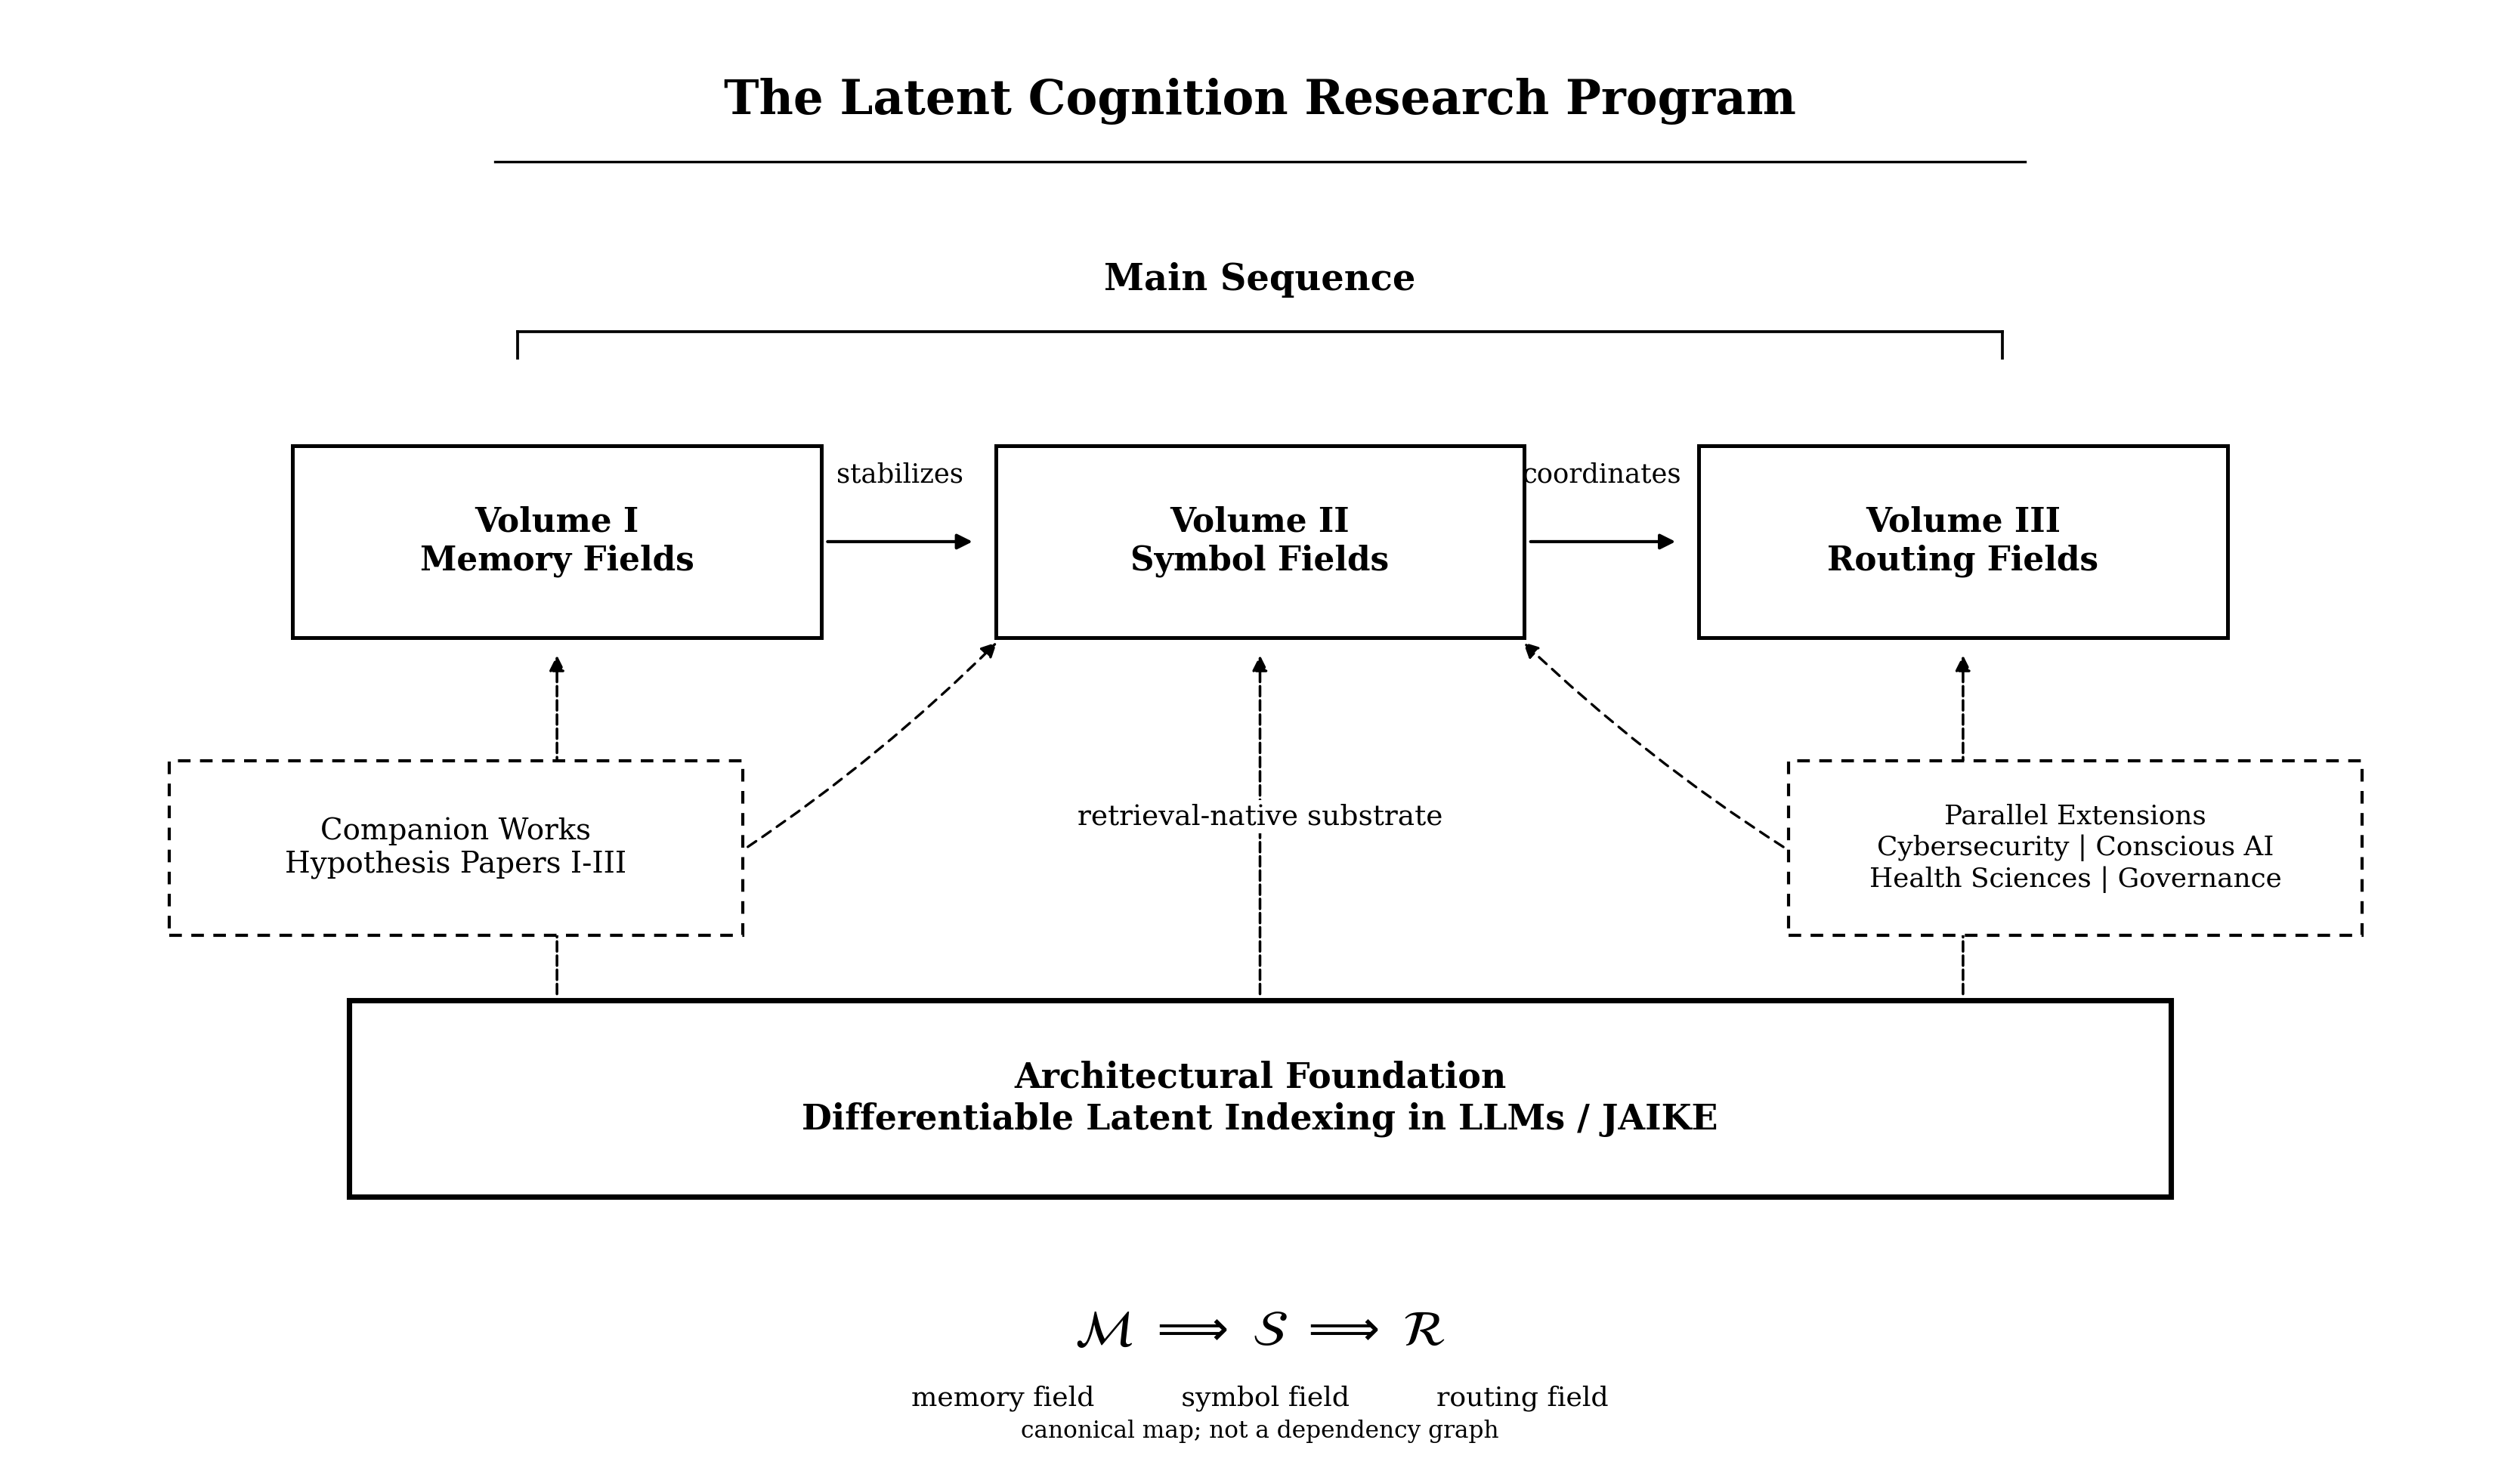
\includegraphics[width=0.88\linewidth]{figures/fig01_trilogy_canonical_map.png}
    \caption{Canonical architecture of the Latent Cognition research program. The DLI-LLM manuscript functions as the architectural foundation, while the three volumes of the Trilogy form the main theoretical sequence from memory fields to symbol fields to routing fields. Companion hypotheses and future extensions orbit the main sequence without replacing it.}
    \label{fig:trilogy-canonical-map}
\end{figure}

\frontchapter{Conceptual Foundations} 
\section*{Core Constructs}

The Trilogy operates on a set of shared constructs that describe internal representations and computational organization in neural architectures. These constructs are not intended to form a closed ontology. They provide a working vocabulary for examining how memory, symbolic stabilization, and routing may interact within latent computational systems.

\textbf{Latent State.}
A latent state is represented as $\mathbf{h}_t \in \latent$, encoding the internal condition of the model at computational step $t$. It is not treated merely as an intermediate activation, but as a structured representational state through which information, context, and transformation history may be partially expressed.

\textbf{Memory Field.}
A memory field, denoted $\MemoryField$, refers to a structured collection of latent representations accessible through differentiable retrieval. Within the Trilogy, the memory field provides the conceptual basis for treating retrieval as an internal representational operation rather than as an external lookup procedure.

\textbf{Symbolic Representation.}
A symbolic representation is denoted as $s \in \symspace$ and refers to a compressed or stabilized encoding derived from latent states. The term does not imply classical symbolic manipulation in the strict sense. Rather, it designates a representational condition in which compressed latent structures acquire sufficient stability to support abstraction, reuse, and interpretation.

\textbf{Routing Function.}
A routing function, denoted $\route{\cdot}{\expertspace}$, governs the allocation of computation across specialized modules, experts, or representational pathways. In this framework, routing is treated not only as an efficiency mechanism, but as a structural principle through which large-scale architectures maintain coherence across distributed computation.

\section*{Structural Relationship}

The Trilogy examines the interaction between these constructs across three stages:

\[
\MemoryField \;\Longrightarrow\; \SymbolField \;\Longrightarrow\; \RoutingField
\]

This progression should not be interpreted as a strict causal chain. Rather, it represents the analytical sequence adopted by the Trilogy. The first stage examines how latent memory may be structured and retrieved. The second stage considers how compressed representations may acquire symbolic stability. The third stage analyzes how routing mechanisms coordinate computation across specialized structures.

The shared hypothesis across the Trilogy is that these constructs are not independent engineering conveniences. They may represent interdependent layers of a broader latent cognitive architecture: memory supplies retrievable structure, symbolic stabilization supplies abstraction, and routing supplies coordinated computational organization.

% Fix: Force continuity so it does NOT reset to 'i'
\clearpage 
\frontchapter{Introduction to the Trilogy} 
% \chapter{Overview of the Trilogy}
\section{Purpose of the Trilogy}

The purpose of \textit{The Latent Cognition Trilogy} is to provide a structured theoretical account of latent computation in contemporary neural architectures. The Trilogy does not attempt to define consciousness, agency, or intelligence in general terms. Its focus is narrower and more architectural: it examines how memory, symbolic stabilization, and routing may operate as interdependent layers within large-scale neural systems.

The central motivation is that many current descriptions of artificial intelligence remain divided between external engineering mechanisms and internal cognitive interpretation. Retrieval is often treated as an external service. Symbolic behavior is often described as an emergent property without sufficient structural explanation. Routing is often framed as an optimization mechanism for scaling model capacity. The Trilogy proposes that these components can be examined together as part of a latent computational architecture.

\section{Volume I: Latent Memory and Retrieval-Native Cognition}

\textbf{Volume I} examines memory as an intrinsic dimension of latent computation. It develops the idea that retrieval may be modeled not only as an external augmentation process, but as an internal operation over latent representational fields. This volume is informed by the architectural foundation developed in \textit{Differentiable Latent Indexing in LLMs: Toward Native Retrieval as a Cognitive Function}, but it extends that foundation into a broader theoretical discussion of memory, access, and latent state organization.

\section{Volume II: Symbolic Stabilization under Compression}

\textbf{Volume II} addresses the conditions under which latent representations acquire symbolic stability. Rather than assuming that symbolic structure appears automatically as an emergent property of scale, this volume examines the role of compression, curriculum, constraint, and representational reuse in shaping stable abstractions. Its central concern is the transition from distributed latent representation to reusable symbolic structure.

\section{Volume III: Hierarchical Routing and Architectural Coordination}

\textbf{Volume III} examines routing as a mechanism of architectural coordination. In large-scale systems, computation is increasingly distributed across specialized components, expert modules, external tools, memory systems, and policy layers. This volume analyzes how hierarchical routing may preserve coherence across such distributed structures and how routing mechanisms may function as part of a broader latent cognitive architecture.

\section{Relation to Companion Works}

\textbf{The Trilogy} is supported by companion works that clarify, formalize, or extend its claims. The DLI-LLM paper provides the architectural foundation for retrieval-native cognition. The companion hypothesis papers isolate specific theoretical claims that orbit the Trilogy without being absorbed into it. This separation allows the main sequence to remain coherent while preserving the broader research program required for future development.

\section{Scope and Limits}

\textbf{The Trilogy} is not presented as a completed theory of artificial cognition. It is a structured research pathway. Its aim is to define a coherent vocabulary, organize related mechanisms, and propose a set of formal and conceptual relationships that can guide future empirical, architectural, and philosophical work.


% =============================================
% MAIN MATTER: THE TRILOGY CORE VOLUMES
% =============================================
\clearpage
\mainmatter % Properly switches layout and resets counter to Arabic (1, 2, 3...)

%--- Title Page ---
\volumetitlepagewithfig
{Volume I: Memory Fields}
{Differentiable Latent Indexing inside Large Language Models}

\vspace*{1cm} % space between title and figures - you control it

\begin{figure}[H] % needs \usepackage{float}
\centering
\begin{minipage}{0.48\textwidth}
    \centering
    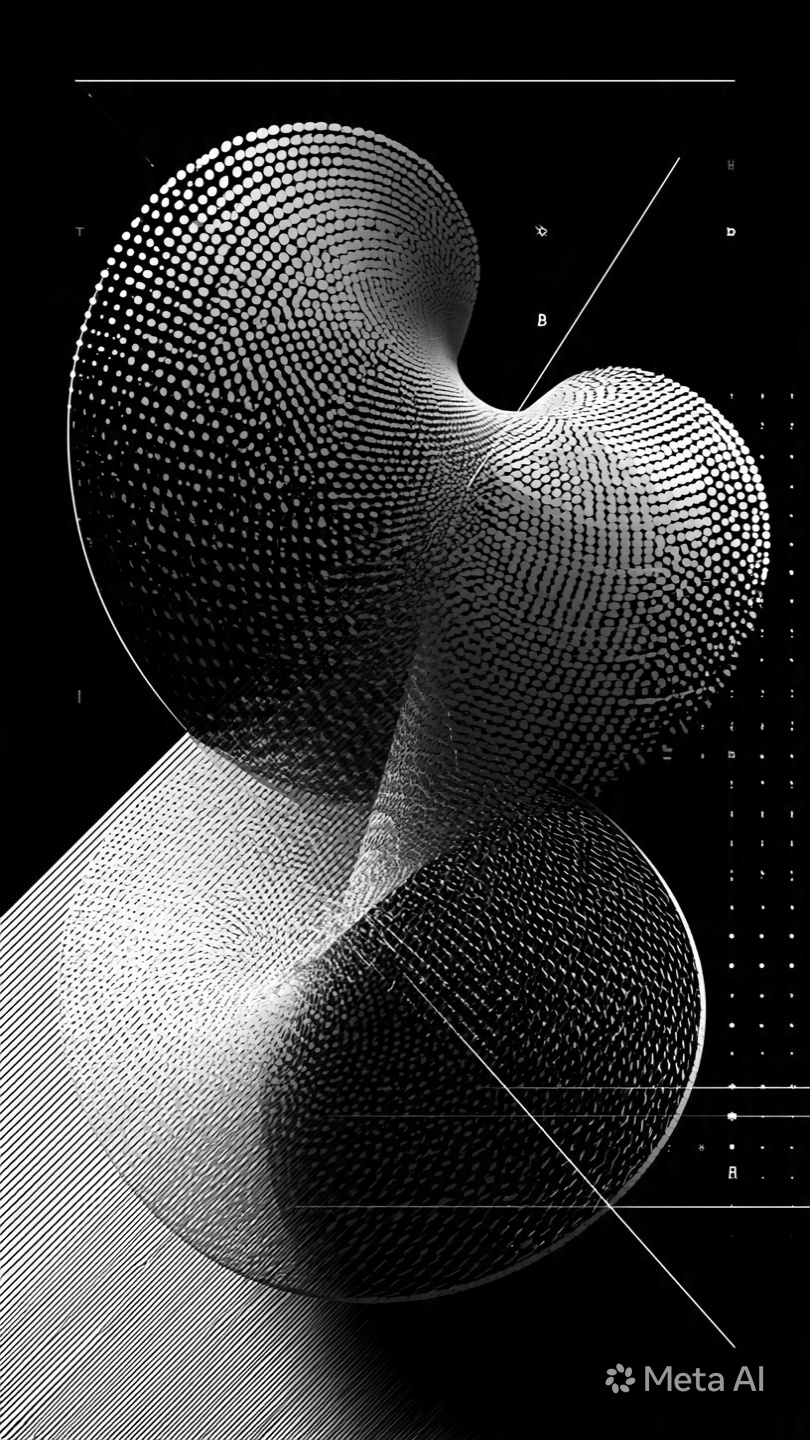
\includegraphics[width=\linewidth,height=0.6\textheight,keepaspectratio]{figures/image-vol1-covera.jpeg}
\end{minipage}
\hfill
\begin{minipage}{0.48\textwidth}
    \centering
    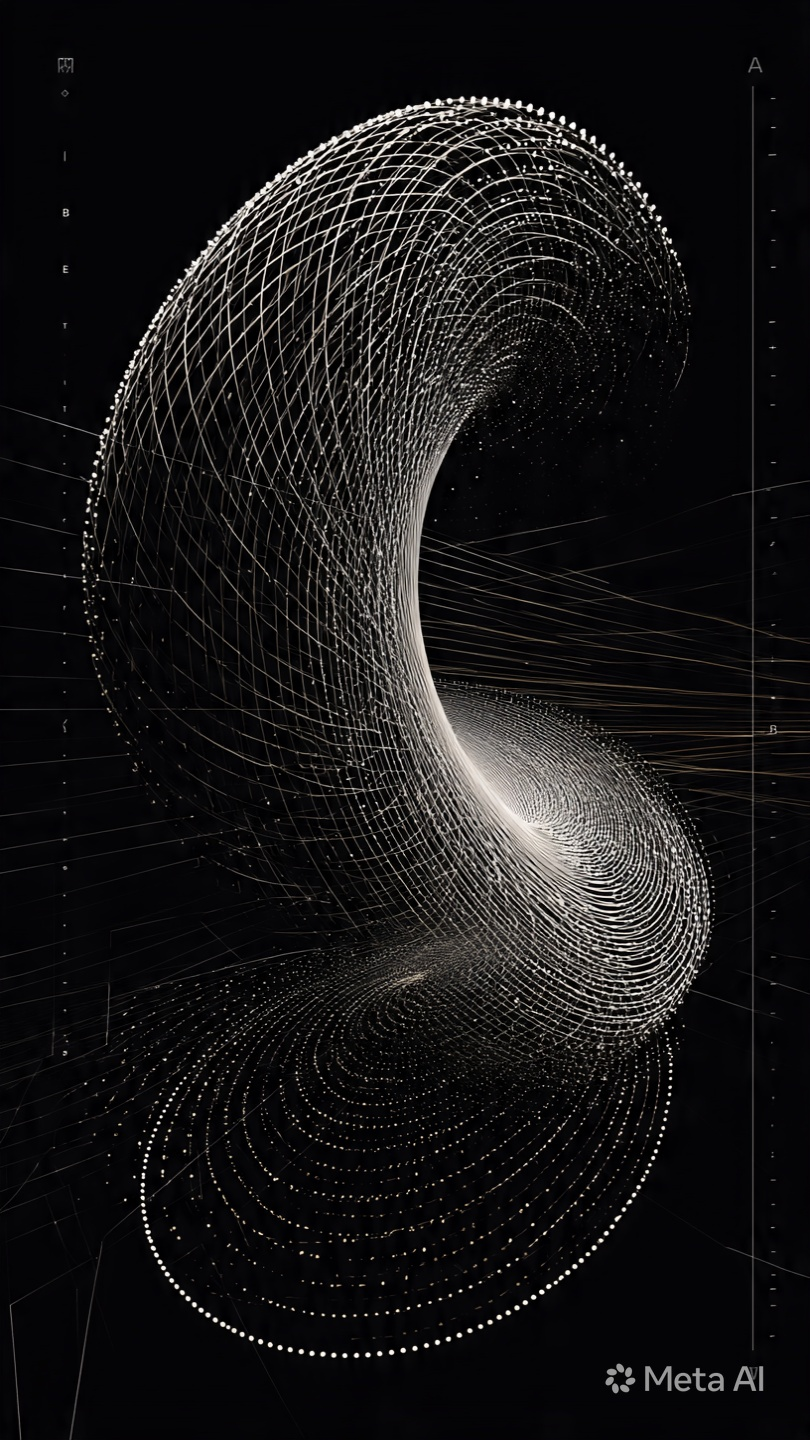
\includegraphics[width=\linewidth,height=0.6\textheight,keepaspectratio]{figures/image-vol1-coverb.jpeg}
\end{minipage}
\end{figure}

 % \footnote{Zinnia Labs Publishing 2026}.

%%\fancyhead{} % clear all header fields
\fancyhead[RO]{\textbf{THE LATENT COGNITION TRILOGY}}
\fancyhead[LE]{\textbf{ZINNIA LABS PUBLISHING}}

%%%%%%%%%%%%%%%%%%%%%%%%%%%%%%%%%
%==================================
% remove \vfill - that's what's pushing to next page
%%%%%%%%%%%%%%%%%%%%%%%%%%%%%%%%%%%
%==================================
\newpage % force next content to start on new page
%%%%%%%%%%%%%%%%%%%%%%%%%%%%%%%%%%%
%==================================
% \vspace{2em}
% \hrule
% \vspace{2em}
% \part{Memory Fields}
% \chapter{Differentiable Latent Indexing inside Large Language Models}

\chapter*{Abstract}
\addcontentsline{toc}{chapter}{Abstract}
This article proposes \textit{Differentiable Latent Indexing} (DLI), a theoretical framework that recontextualizes memory retrieval not as an external utility appended to a language model, but as a native, differentiable function inside the computational pathway of Large Language Models (LLMs). By treating the latent space as a structured information field, the article derives formal retrieval operators that integrate memory access directly into the model's forward pass.

The central claim is that the conventional separation between storage and processing introduces architectural inefficiencies that limit the development of autonomous and cognitively organized AI systems. In current retrieval-augmented designs, the model, retriever, embedding store, and generator often remain operationally coupled but mathematically discontinuous. DLI instead proposes a shared latent memory substrate in which retrieval, routing, and representation learning are jointly optimized.

This work is presented as a conceptual research article. It does not claim empirical validation. Instead, it establishes mathematical scaffolding, explicit propositions, falsification conditions, implementation pathways, and expected failure modes for future experimental work. In doing so, it serves as the first component of a broader research program investigating the internal organization of machine cognition.

\noindent \textit{Keywords: Differentiable Latent Indexing (DLI); Large Language Models (LLMs); Retrieval-Augmented Generation (RAG); Cognitive Architectures; Neural Retrieval; Differentiable Memory; Transformer Models; Cognitive Complete AI; Hypothesis-Extension Research; Artificial Intelligence Theory.}

\section*{Position within the Research Program}

This manuscript constitutes Volume I of \textit{The Latent Cognition Trilogy}. It develops the memory layer of the broader research program by formalizing Differentiable Latent Indexing (DLI) as a candidate mechanism for retrieval-native cognition inside Transformer-based systems.

The closely related manuscript \textit{Differentiable Latent Indexing in LLMs: Toward Native Retrieval as a Cognitive Function}, submitted to the \textit{Journal of Artificial Intelligence and Knowledge Engineering}, provides the formal architectural foundation for this volume. The present text adapts and extends that foundation within the larger Trilogy sequence, where memory, symbolic stabilization, and hierarchical routing are treated as interdependent layers of latent cognition.

Accordingly, Volume I should not be read as a companion hypothesis paper. It is the opening movement of the Trilogy. The companion hypothesis papers occupy a separate position: they isolate specific claims that support, constrain, or extend the main sequence without replacing it.


\section*{Proposition 1: Retrieval Efficiency Gain}
If DLI provides a meaningful internal memory mechanism, models augmented with DLI should demonstrate improved performance on tasks requiring long-range dependency resolution compared with baseline transformers of equivalent parameter count.

\textbf{Falsification condition:} If no statistically significant improvement is observed across controlled benchmarks, the hypothesis that internally differentiable retrieval improves effective memory capacity is weakened.

\section*{Proposition 2: Latent Clustering Stability}
DLI should induce measurable clustering in latent representations corresponding to recurrent semantic structures.

\textbf{Falsification condition:} If latent representations remain uniformly distributed or indistinguishable from baseline attention patterns, the claim of structured internal memory is not supported. To mathematically verify this organization, the spatial distribution of the latent memory field can be monitored via a localized Silhouette Coefficient ($S$). For a cluster of recurrent semantic structures $C$, the stability metric is formalized as:

\begin{equation}
S(M^{(\ell)}) = \frac{1}{|C|} \sum_{i \in C} \frac{b(i) - a(i)}{\max(a(i), b(i))},
\end{equation}

where $a(i)$ represents the mean intra-cluster distance of representation $i$, and $b(i)$ represents the mean nearest-cluster distance to any other semantic partition. The proposition holds if and only if $S(M^{(\ell)}) > \epsilon$ as training progress approaches convergence, where $\epsilon$ is the baseline uniform distribution threshold.

\section*{Proposition 3: Retrieval-Induced Drift}
Repeated retrieval operations should introduce measurable drift in latent state trajectories.

\textbf{Falsification condition:} If no measurable deviation from baseline forward-pass dynamics is observed, the proposed retrieval interaction is not functionally distinct.

\section*{Introduction}

The present volume inaugurates \textit{The Latent Cognition Trilogy}, a sequence of conceptual research works centered on latent cognition in artificial systems. Volume I formalizes \textit{Differentiable Latent Indexing} (DLI) as a native retrieval mechanism inside Transformer-based language models. It does not report experimental results; rather, it formalizes, elaborates, and critically develops a theoretical architecture in which memory retrieval becomes part of the model's differentiable computational pathway.

The paper extends the \textbf{Differentiable Latent Indexing inside Large Language Models (DLI-LLM)} hypothesis by positioning it as an architectural paradigm for retrieval inside Transformer computation. 

\textbf{Volume II} examines the conditions under which compressed latent representations acquire symbolic stability under curriculum, compression, and structural constraint. \textbf{Volume III} extends the sequence by analyzing hierarchical routing as a mechanism of architectural coordination across specialized computational components. Together, these papers aim to establish a conceptual lineage for AI systems that treats memory, routing, representation, and control as interdependent components of machine cognition.

This article was developed in response to a hypothesis generated by the Academia.edu AI-assisted scientific modeling platform. The original hypothesis proposed a learnable, differentiable memory-retrieval mechanism embedded directly within Transformer layers. Rather than treating that hypothesis as a fixed endpoint, the present paper treats it as a conceptual seed: a starting point for examining the architectural, cognitive, mathematical, and safety implications of internalized retrieval.

The problem space addressed here is the separation between parametric memory, stored within model weights, and non-parametric memory, retrieved through external documents, embedding stores, or vector databases. Retrieval-augmented generation has improved factual grounding by combining sequence-to-sequence generation with external dense retrieval \cite{Lewis2021}. Related approaches, including nearest-neighbor language models and memorizing transformers \cite{Wu2022}, demonstrate that language models can benefit from access to stored representations beyond the immediate context window \cite{Khandelwal2020, Wu2022}. However, these approaches also preserve a structural separation between the model's internal computation and the retrieval substrate.

This separation produces three persistent architectural constraints:

\begin{enumerate}
    \item latency and bandwidth trade-offs between inference and retrieval operations;
    \item semantic drift between retrieved information and the evolving internal context of the model; and
    \item limited gradient flow between evidence selection, memory access, and downstream reasoning.
\end{enumerate}

DLI proposes a departure from this pattern. It introduces a differentiable memory module embedded within Transformer layers and trained jointly with the model. Memory queries are formulated from hidden states, routed to a latent key-value memory, and fused back into the model via gated integration. Product quantization provides a possible mechanism for scalable approximate search, while gating regulates when retrieved memory should influence the hidden state \cite{Jgou2011, Johnson2021, Lepikhin2020}.

By situating retrieval as an internalized cognitive function, DLI reframes memory access as part of the model's own computational graph rather than as an external service call. The resulting architecture is not merely an optimization of retrieval-augmented generation. It is a theoretical proposal to unify attention, memory, and representational control within Transformer-based systems.

\section*{Contributions}
This work contributes the following elements:

\begin{enumerate}
    \item a unified architectural hypothesis that integrates latent memory directly into Transformer computation;
    \item a mathematical definition of differentiable retrieval, routing, and gated fusion;
    \item a conceptual implementation blueprint for internal retrieval during inference;
    \item a comparative analysis connecting DLI to retrieval-augmented generation, kNN language models, differentiable memory systems, recurrent memory transformers \cite{Wu2022}, and cognitive architectures; and
    \item a foundation for the broader research program developed in the \textit{Latent Cognition Trilogy}.
\end{enumerate}

\section{Overview of the Paper}
Section 2 develops the methodological foundation by decomposing the originating DLI-LLM hypothesis into its constituent architectural claims. Section 3 presents theoretical predictions and falsifiable implications. Section 4 develops the mathematical formulation of Differentiable Latent Indexing. Section 5 provides a conceptual implementation blueprint and comparative literature analysis. Section 6 discusses broader implications for cognitive modeling, learning dynamics, safety, and cognitive-complete Transformer architectures.

\section{The Unified Cognitive Operator Field}

To transcend the architectural discontinuities inherent in decoupled Retrieval-Augmented Generation (RAG) paradigms, we formalize the autonomous system not as an agglomeration of discrete pipelines, but as a unified cognitive operator space denoted by $\mathcal{A}$. The total cognitive state transition is governed by the triple operator configuration:

\begin{equation}
\mathcal{A} = (M, S, R)
\end{equation}

where $M$ represents the continuous Latent Memory operator, $S$ denotes the discrete Symbolic Mapping operator, and $R$ defines the Topological Reasoning and Routing operator. 

\subsection{\texorpdfstring{Mathematical Formalization of the Memory Operator $M$}{Mathematical Formalization of the Memory Operator M}}

Rather than treating the latent space $\mathcal{X} \subset \mathbb{R}^d$ as a static repository for vector retrieval, we define it as a continuous, differentiable information field. Let $\psi(t) \in \mathcal{X}$ represent the current latent trajectory of the model's forward pass at computational step $t$. The memory operator $M$ maps the input state and the historical manifold directly into a continuous retrieval field without invoking non-differentiable $k$-NN lookup bottlenecks:

\begin{equation}
M: \mathcal{X} \times \mathcal{H} \to \mathcal{X}
\end{equation}

We define the action of $M$ on a latent state $\psi(t)$ conditioned on an informational reservoir matrix $\mathcal{M}_{field}$ as:

\begin{equation}
M(\psi(t); \mathcal{M}_{field}) = \nabla_{\psi} \int_{\Omega} \mathcal{K}(\psi(t), \omega) \, d\mu(\omega)
\end{equation}

Where $\mathcal{K}$ is a non-linear kernel quantifying the field density over the informational domain $\Omega$, and $\mu(\omega)$ is the probability measure of the latent distribution. This formulation ensures that memory retrieval is natively integrated as a gradient-descent optimized trajectory within the forward pass itself.

\subsection{\texorpdfstring{Boundary Interface: $M \longrightarrow S \longrightarrow R$}{Boundary Interface: M -> S -> R}}

The structural integrity of $\mathcal{A}$ depends on the seamless composition of its operators. The output of the continuous memory operator $M$ must enforce strict boundary constraints to parameterize the discrete symbolic operator $S$, which in turn formats the input for the reasoning operator $R$. 

Let $\mathcal{S}_{space}$ represent the discrete, invariant vocabulary or operational action space. The transition is governed by the composition:

\begin{equation}
\Psi_{total} = R \circ S \circ M(\psi(t))
\end{equation}

We establish the exact operational boundaries below:
\begin{enumerate}
    \item \textbf{Continuous-to-Discrete Mapping ($M \to S$):} The output vector field $M(\psi(t))$ parameterizes a categorical probability distribution over $\mathcal{S}_{space}$. The operator $S$ projects this field onto a discrete manifold via an audited projection operator $\Pi_{\mathcal{S}}$:
    \begin{equation}
    S(M(\psi(t))) = \Pi_{\mathcal{S}} \left( \sigma \left( W_s \cdot M(\psi(t)) \right) \right)
    \end{equation}
    where $\sigma$ represents the softmax function and $W_s$ is the learnable transformation matrix aligning memory fields with symbolic invariants.
    
    \item \textbf{Symbolic-to-Reasoning Routing ($S \to R$):} The discrete sequence generated by $S$ dictates the topological routing trajectory inside $R$. The reasoning operator $R$ evaluates the causal validity of the state sequence, preventing model collapse by restricting transitions to permitted paths defined by the architectural prior:
    \begin{equation}
    R(S(M(\psi(t)))) = \oint_{\Gamma} \mathcal{F}\left(S \circ M\right) \, dz \equiv 0
    \end{equation}
    where $\Gamma$ represents a closed computational loop, forcing topological conservation of the cognitive audit trail.
\end{enumerate}

\section{Epistemological Framework and Empirical Falsification}

In alignment with classical scientific rationalism, a foundational architectural theory must explicitly define its conditions for empirical falsification. We reject the purely descriptive, ad-hoc post-processing evaluation metrics that characterize modern engineering benchmarks. Instead, we formulate three mathematically rigorous propositions that expose the continuous field dynamics of the triple operator configuration $\mathcal{A} = (M, S, R)$ to direct empirical scrutiny.

\subsection{Proposition I: The Field Collapse Invariant}

Let $\mathcal{M}_{field}$ be an informational reservoir matrix with local density distribution $\mu(\omega)$. If an external token-based retrieval paradigm (e.g., standard dense vector retrieval or $k$-NN lookup) is superimposed onto the continuous latent trajectory $\psi(t)$, the informational entropy $H$ of the system must exhibit non-linear degradation under out-of-distribution (OOD) testing.

We state that the continuous memory operator $M$ eliminates model collapse if and only if the latent field curvature satisfies the invariant:

\begin{equation}
\lim_{\Delta \Omega \to 0} \mathbb{E}_{\psi} \left[ \| M(\psi(t)) - \psi(t) \|^2 \right] \le \gamma \cdot \mathcal{H}(\mathcal{M}_{field})
\end{equation}

where $\gamma$ is an architectural constant and $\mathcal{H}$ is the structural information capacity of the manifold. 
\paragraph{Falsification Condition:} This proposition is empirically falsified if a decoupled vector-store architecture can maintain topological consistency and zero auto-regressive degradation under sequential context-window saturation ($\ge 10^6$ tokens) without dynamic parameters fine-tuning or continuous memory-field field re-indexing.

\subsection{Proposition II: Boundary Transition Degeneracy}

The continuous-to-discrete projection mapping handled by the Symbolic operator $S$, denoted as $S(M(\psi(t)))$, preserves the causal alignment of the cognitive audit trail. Let $\Pi_{\mathcal{S}}$ be the audited projection operator onto the discrete manifold. The transition error $\mathcal{E}_{trans}$ is bounded by the spectral radius $\rho$ of the transformation matrix $W_s$:

\begin{equation}
\mathcal{E}_{trans} = \| \Pi_{\mathcal{S}} ( \sigma (W_s \cdot M(\dots) ) ) - S_{true} \| \le \lambda \cdot \rho(W_s)^{-1}
\end{equation}

\paragraph{Falsification Condition:} This proposition is empirically falsified if a stochastic, un-audited token routing system (e.g., mixture-of-experts or standard temperature-scaled sampling) achieves deterministic invariance in symbolic state transitions over an unconstrained adversarial execution domain.

\subsection{Proposition III: Topological Conservation and Scaling Limits}

The Reasoning and Routing operator $R$ enforces a closed loop integral condition on the symbolic state sequences generated by $S$:

\begin{equation}
\oint_{\Gamma} \mathcal{F}\left(S \circ M\right) \, dz \equiv 0
\end{equation}

This implies that the cognitive audit trail must conserve informational momentum, preventing semantic drifting across deep inference chains.
\paragraph{Falsification Condition:} This proposition is empirically falsified if an open-loop, non-differentiable retrieval architecture can achieve a complex multi-hop inference success rate exceeding $95\%$ while operating under hard real-time latency limits ($T \le 15\text{ms}$) across completely unseen multi-domain network topologies.

\section{Theoretical Construction and Implications}
This paper does not report empirical results. Its contribution is the theoretical development of a Transformer-based architecture through structured hypothesis modeling. The starting point is the DLI-LLM hypothesis, which is decomposed into a set of architectural claims and then expanded into a formal framework suitable for future empirical study.

\subsection{Hypothesis Decomposition}
The original hypothesis can be decomposed into four architectural claims:

\begin{enumerate}
    \item a differentiable memory module embedded inside Transformer layers;
    \item a product-quantized memory structure for scalable approximate retrieval;
    \item a shared latent vector space for token-level representations and document-level embeddings; and
    \item a learned query-gating mechanism for retrieval triggering and fusion control.
\end{enumerate}

Each claim has precedent in adjacent literature but differs in the proposed integration. Neural Turing Machines \cite{Graves2014} and Differentiable Neural Computers introduced differentiable access to external memory \cite{Graves2014, Graves2016}. Memory-augmented neural networks demonstrated rapid assimilation of new examples through content-based memory access \cite{Santoro2016}. Recurrent memory transformers and memorizing transformers later adapted memory mechanisms to Transformer-based language modeling \cite{Bulatov2022, Wu2022}. DLI differs from these systems in that it treats latent retrieval as an internal, trainable component of the Transformer layer itself.

\subsection{Architectural Modeling}
The hypothesis is extended into a multi-stage retrieval loop inside the forward pass. At a high level, the current hidden state is used to generate a query vector. That query vector retrieves top-$k$ value vectors from a latent key--value memory. The retrieved representation is then fused back into the model through a learned routing gate. This loop creates a differentiable pathway between hidden-state evolution and memory access.

The proposed retrieval loop contains three major operations:

\begin{enumerate}
    \item cross-layer memory interpolation, in which retrieval results influence subsequent Transformer layers;
    \item sparse top-$k$ selection, allowing retrieval to remain computationally bounded; and
    \item internal--external evidence arbitration, in which latent memory competes with or complements the local attention pathway.
\end{enumerate}

To visualize the core concept, \textbf{Figure}~\ref{fig:dli-architecture} introduces the proposed DLI-LLM architecture.

\begin{figure}
    \centering
    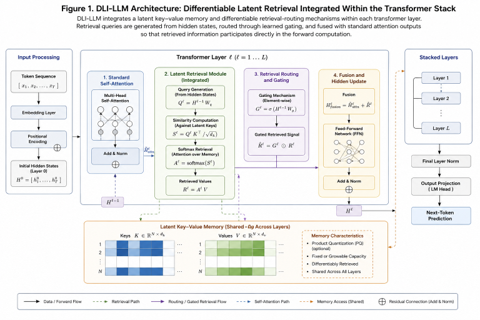
\includegraphics[width=0.72\linewidth]{figures/Picture1a.png}
    \caption{Differentiable Latent Indexing architecture. The diagram illustrates how latent key--value memory slots are queried from the current hidden state and fused back into the Transformer attention pathway during the forward pass.}
    \label{fig:dli-architecture}
\end{figure}

\subsection{Comparative Contextualization}
DLI intersects with several existing research lines. Retrieval-augmented generation combines parametric sequence generation with non-parametric document retrieval \cite{Lewis2021}. kNN-LM interpolates language-model predictions with nearest-neighbor lookup over stored representations \cite{Khandelwal2020}. Memorizing Transformers store recent key--value representations for later lookup \cite{Wu2022}. Dense passage retrieval systems optimize learned representations for open-domain question answering \cite{Qu2021}. Memory-augmented neural networks and differentiable memory systems demonstrate that memory can be made trainable through differentiable addressing \cite{Graves2014, Graves2016, Santoro2016}.

DLI draws on all of these traditions but shifts the point of integration. Rather than positioning retrieval as a pre-generation evidence step or a post-hoc interpolation mechanism, DLI treats retrieval as part of the Transformer layer's representational dynamics. The implication is architectural: the model does not merely consult memory; it computes through memory.

\section{Theoretical Predictions}
Because no DLI-LLM model is implemented in this article, the following claims should be read as theoretical predictions rather than empirical results. They define expected behaviors that future experimental studies should attempt to confirm, refine, or falsify.

\begin{itemize}
    \item \textbf{Retrieval latency.} By integrating retrieval into the forward pass, DLI-LLM is expected to reduce the external retriever bottleneck characteristic of conventional RAG architectures. Approximate nearest-neighbor methods and GPU-accelerated similarity search provide a plausible basis for this efficiency claim \cite{Jgou2011, Johnson2021}.
    \item \textbf{Grounding stability.} Stable latent memory may reduce hallucination in knowledge-intensive tasks by narrowing the distance between retrieved evidence and internal representation. This prediction is motivated by improvements observed in retrieval-augmented generation and nearest-neighbor language modeling \cite{Lewis2021, Khandelwal2020}.
    \item \textbf{Generalization through memory retention.} Because latent memory slots are differentiably integrated into Transformer layers, DLI may reproduce some of the generalization-through-memorization dynamics observed in kNN-LM and memorizing transformers \cite{Khandelwal2020, Wu2022}.
    \item \textbf{Few-shot adaptation.} Learned gating may improve adaptation under limited supervision by controlling when retrieved memory should alter the hidden state, a behavior related to memory-augmented few-shot learning \cite{Santoro2016}.
    \item \textbf{Cross-layer coherence.} Query propagation across layers may improve long-context coherence by maintaining retrieval continuity over successive transformations, complementing trends in recurrent memory transformers \cite{Bulatov2022}.
\end{itemize}

The predicted failure modes are equally important:

\begin{itemize}
    \item \textit{Memory saturation}: fixed-size latent memory may become overloaded under high document or representation density \cite{Graves2014, Wu2022}.
    \item \textit{Value-vector redundancy}: top-$k$ retrieval in high-dimensional latent spaces may return semantically redundant vectors, reducing effective retrieval precision without pruning, compression, or quantization \cite{Jgou2011, Johnson2021}.
    \item \textit{Context misalignment}: retrieval queries may drift when cross-layer propagation interacts poorly with earlier representations, particularly in recurrent or persistent-memory settings \cite{Bulatov2022}.
    \item \textit{Opacity of internal retrieval}: once retrieval is internalized, the evidentiary path may become harder to inspect than in externally mediated RAG systems.
\end{itemize}

\textbf{Figure}~\ref{fig:rag-pipeline} contrasts the conventional retrieval-augmented generation pattern with the internalized retrieval logic proposed by DLI.

\begin{figure}
    \centering
    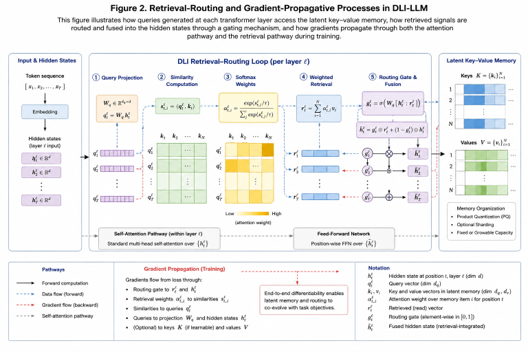
\includegraphics[width=0.72\linewidth]{figures/Picture2a.png}
    \caption{Standard retrieval-augmented generation pipeline. In conventional RAG, retrieval remains externally mediated through a document index or vector store before generation. DLI proposes to move part of this retrieval logic into the model's differentiable computation path.}
    \label{fig:rag-pipeline}
\end{figure}

\section{Mathematical Framing of Differentiable Latent Indexing}
To transition from conceptual architecture to a formally analyzable model, this section expresses DLI-LLM as a minimal extension of standard Transformer notation. Let $h_t^{(\ell)} \in \mathbb{R}^{d}$ denote the hidden state at token position $t$ and layer $\ell$, following the general structure of attention-based Transformer computation \cite{Vaswani2017}. DLI augments this computation with a latent key--value memory and a differentiable routing mechanism.

\subsection{Latent Key--Value Memory}
For each layer $\ell$, define a latent memory bank:

\begin{equation}
M^{(\ell)} = \{(k_i^{(\ell)}, v_i^{(\ell)})\}_{i=1}^{N},
\end{equation}

where $k_i^{(\ell)} \in \mathbb{R}^{d_k}$ is a memory key and $v_i^{(\ell)} \in \mathbb{R}^{d_v}$ is the corresponding memory value. The memory bank may contain internal token-derived representations, document-derived embeddings, or a hybrid of both. This formulation extends differentiable memory systems by embedding memory within layer-level computation rather than attaching it as a separate controller \cite{Graves2014,Graves2016,Santoro2016}.

\subsection{Query Projection}
A learned projection maps the current hidden state into a retrieval query:

\begin{equation}
q_t^{(\ell)} = W_q^{(\ell)} h_t^{(\ell)} + b_q^{(\ell)}.
\end{equation}

This query projection is analogous to attention-based addressing but is directed toward persistent latent memory rather than only toward positions within the active context window \cite{Bahdanau2016, Vaswani2017}.

\subsection{Similarity and Sparse Retrieval}
The model computes retrieval logits through a similarity function:

\begin{equation}
s_i^{(\ell)} = \frac{q_t^{(\ell)} \cdot k_i^{(\ell)}}{\sqrt{d_k}}
\end{equation}

A sparse top-$k$ selection operator restricts retrieval to the most relevant memory entries: 

\begin{equation}
\alpha_i^{(\ell)} = \frac{\exp(s_i^{(\ell)}/\tau)\mathbf{1}[i \in \operatorname{TopK}(s^{(\ell)}, k)]}{\sum_{j \in \operatorname{TopK}(s^{(\ell)}, k)} \exp(s_j^{(\ell)}/\tau)}
\end{equation}

where $\tau$ is a temperature parameter and $\alpha_i^{(\ell)}$ is the differentiable retrieval weight assigned to memory slot $i$. Product quantization may be used to approximate key search at scale \cite{Jgou2011, Johnson2021}.

\subsection{Retrieved Representation}
The retrieved latent representation is computed as a weighted sum of memory values:

\begin{equation}
r_t^{(\ell)} = \sum_{i=1}^{N} \alpha_i^{(\ell)} v_i^{(\ell)}.
\end{equation} 

This operation turns memory access into a differentiable aggregation step, preserving gradient flow through the retrieval distribution.

\subsection{Gated Fusion}
A learned gate controls the influence of retrieved memory on the evolving hidden state:

\begin{equation}
g_t^{(\ell)} = \sigma\left(W_g^{(\ell)}[h_t^{(\ell)} \parallel r_t^{(\ell)}] + b_g^{(\ell)}\right),
\end{equation}

where $[h_t^{(\ell)} \parallel r_t^{(\ell)}]$ denotes vector concatenation and $\sigma$ is the logistic sigmoid. The fused representation is then:

\begin{equation}
\tilde{h}_t^{(\ell)} = \operatorname{LayerNorm}\left(h_t^{(\ell)} + g_t^{(\ell)} \odot r_t^{(\ell)}\right).
\end{equation}

This gating operation connects DLI to conditional computation and mixture-style routing, while preserving a layer-local mechanism for regulating memory influence \cite{Lepikhin2020, Bulatov2022}.

\subsection{Training Objective}
A conceptual DLI training objective can be written as:

\begin{equation}
\mathcal{L}_{DLI} = \mathcal{L}_{LM} + \lambda_s \mathcal{L}_{sparse} + \lambda_m \mathcal{L}_{memory} + \lambda_g \mathcal{L}_{gate}
\end{equation}

where $\mathcal{L}_{LM}$ is the standard language modeling loss, $\mathcal{L}_{sparse}$ regularizes retrieval selectivity by penalizing the entropy of the allocation profile $\alpha$, $\mathcal{L}_{memory}$ regulates memory coherence or redundancy, and $\mathcal{L}_{gate}$ discourages uncontrolled reliance on retrieved values. The exact form of these terms is an empirical design question, but the formulation clarifies where future implementations may intervene.

\subsection{Gradient Flow and Optimization Continuity}
Because the sparse selection operator $\operatorname{TopK}(\cdot)$ introduces a non-differentiable boundary, gradient continuity along the retrieval pathway is maintained via softmax weighting across the chosen partition. The partial derivative of the fused representation $\tilde{h}_t^{(\ell)}$ with respect to the memory keys $k_i^{(\ell)}$ propagates directly through the similarity scaling:

\begin{equation}
\frac{\partial \tilde{h}_t^{(\ell)}}{\partial k_i^{(\ell)}} = g_t^{(\ell)} \odot v_i^{(\ell)} \left( \frac{\partial \alpha_i^{(\ell)}}{\partial s_i^{(\ell)}} \right) \left( \frac{q_t^{(\ell)}}{\sqrt{d_k}} \right).
\end{equation}

This formalizes a continuous, uninterrupted backward pass from downstream language modeling errors directly into the latent memory coordinates, allowing the index structure to co-evolve with parametric transformations without a separate optimization loop.

\textbf{Figure}~\ref{fig:gradient-pathways} illustrates how gradients propagate through the attention and retrieval pathways during training.

\begin{figure}
    \centering
    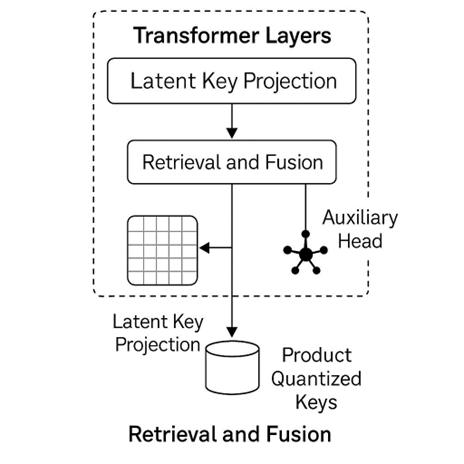
\includegraphics[width=0.72\linewidth]{figures/Picture3.png}
    \caption{Gradient pathways in Differentiable Latent Indexing. Query projection, similarity computation, sparse retrieval weighting, routed memory integration, and gated fusion remain within the differentiable computation graph, allowing latent memory to co-evolve with Transformer parameters.}
    \label{fig:gradient-pathways}
\end{figure}
\begin{algorithm}[H] 
    \caption{Differentiable Latent Indexing Loop}
    \label{alg:dli-loop}

    \smallskip
    \textbf{Input:} hidden state $h_t^{(\ell)}$, latent memory $M^{(\ell)} = \{(k_i^{(\ell)}, v_i^{(\ell)})\}_{i=1}^{N}$, parameters $W_q^{(\ell)}$, $W_g^{(\ell)}$, top-$k$ value, temperature $\tau$.
    
    \textbf{Output:} fused representation $\tilde{h}_t^{(\ell)}$.
    \smallskip

    \begin{enumerate}
        \item Compute retrieval query: $q_t^{(\ell)} \leftarrow W_q^{(\ell)}h_t^{(\ell)} + b_q^{(\ell)}$.
        \item Compute similarity scores: $s_i^{(\ell)} \leftarrow q_t^{(\ell)} \cdot k_i^{(\ell)} / \sqrt{d_k}$.
        \item Select top-$k$ memory slots according to $s_i^{(\ell)}$.
        \item Compute retrieval weights: $\alpha^{(\ell)} \leftarrow \operatorname{softmax}(s^{(\ell)}/\tau)$ over selected slots.
        \item Retrieve latent value: $r_t^{(\ell)} \leftarrow \sum_i \alpha_i^{(\ell)}v_i^{(\ell)}$.
        \item Compute routing gate: $g_t^{(\ell)} \leftarrow \sigma(W_g^{(\ell)}[h_t^{(\ell)} \parallel r_t^{(\ell)}] + b_g^{(\ell)})$.
        \item Fuse retrieved memory with hidden state: $\tilde{h}_t^{(\ell)} \leftarrow \operatorname{LayerNorm}(h_t^{(\ell)} + g_t^{(\ell)} \odot r_t^{(\ell)})$.
        \item Return $\tilde{h}_t^{(\ell)}$.
    \end{enumerate}
\end{algorithm}

Although this paper is theoretical, an implementable DLI prototype would require four design stages.

\subsection{Memory Construction}
Document embeddings, token representations, or intermediate hidden states would be transformed into latent key--value banks. Product quantization could then be applied to compress memory and enable approximate retrieval at scale \cite{Jgou2011, Johnson2021}.

\subsection{Quantized Latent Indexing Mechanics}
To prevent the $\text{TopK}$ operations from scaling linearly $\mathcal{O}(N)$ with the size of the latent memory repository, the key space is structured using Product Quantization (PQ). The high-dimensional key space $\mathbb{R}^{d_k}$ is decomposed into $M$ orthogonal subspaces:

\begin{equation}
\mathbb{R}^{d_k} = \mathbb{R}^{d_s} \times \mathbb{R}^{d_s} \times \dots \times \mathbb{R}^{d_s},
\end{equation}

where $d_s = d_k / M$. Each subspace is quantized into $K^*$ centroids using a learned codebook. During the forward pass, the query projection $q_t^{(\ell)}$ is similarly sliced into $M$ sub-vectors. Similarity estimation $s_i^{(\ell)}$ is then executed via asymmetric distance computation (ADC) using pre-calculated look-up tables. This reduces the computational overhead of the internalized retrieval phase to a collection of parallel cache lookups, maintaining a highly bounded inference budget.

\subsection{Layer Integration}
A DLI block would be inserted after self-attention or between attention and feed-forward sublayers. The routing gate would determine whether retrieved values should influence the hidden state. This placement allows DLI to function as a memory-aware extension of Transformer computation rather than as a separate retrieval pipeline.

\subsection{Training and Fine-Tuning}
Training would jointly optimize language modeling, retrieval selectivity, memory coherence, and gating behavior. In a pre-training setting, memory slots could evolve with the model. In a fine-tuning setting, selected memory banks could be frozen, swapped, or domain-adapted.

\subsection{Inference Behavior}
During inference, DLI could operate through frozen or partially updateable memory. Sparse top-$k$ retrieval would limit computational overhead. Memory swapping could support domain-specific deployment, while gating thresholds could regulate when latent memory influences generation.

\subsection{Evaluation Plan}
A future empirical study should compare DLI-augmented models against baseline Transformers, RAG models, kNN-LM variants, and memorizing transformers. Evaluation should include latency overhead, retrieval precision, hallucination rates, long-context coherence, memory saturation, and ablation studies that independently disable routing, memory access, or quantization.

\section{Comparative Literature Analysis}
\textbf{Table}~\ref{tab:comparative-architectures} summarizes the position of DLI relative to adjacent architectures.

\begin{table}[ht!]
\centering
\small
\begin{tabular}{p{0.26\linewidth}p{0.36\linewidth}p{0.30\linewidth}}
\hline
\textbf{Architecture} & \textbf{Relation to DLI} & \textbf{Limitation Relative to DLI} \\
\hline
Retrieval-Augmented Generation & Combines parametric generation with non-parametric retrieval \cite{Lewis2021}. & Retrieval is typically external to the Transformer computation graph. \\
\hline
$k$NN-LM & Interpolates language-model predictions with nearest-neighbor lookup \cite{Khandelwal2020}. & Retrieval is post-hoc and not trained as an internal layer function. \\
\hline
Memorizing Transformers & Store and retrieve recent key--value representations \cite{Wu2022}. & Memory improves context use but remains distinct from document-level latent unification. \\
\hline
Neural Turing Machines / DNC & Demonstrate differentiable memory addressing \cite{Graves2014, Graves2016}. & Designed as general memory controllers rather than layer-native LLM retrieval modules. \\
\hline
Memory-Augmented Neural Networks & Support rapid assimilation of new examples \cite{Santoro2016}. & Primarily oriented toward few-shot learning rather than Transformer-internal retrieval. \\
\hline
Recurrent Memory Transformer & Uses memory tokens for long-sequence processing \cite{Bulatov2022}. & Memory persistence is present, but explicit latent key--value retrieval control is limited. \\
\hline
Dense Passage Retrieval / RocketQA & Optimizes learned representations for retrieval \cite{Qu2021}. & Retrieval occurs outside the model's internal forward computation. \\
\hline
Product-Quantized Vector Search & Provides scalable approximate search \cite{Jgou2011, Johnson2021}. & Supplies retrieval infrastructure but not a cognitive or Transformer-layer architecture. \\
\hline
\end{tabular}
\caption{Comparative analysis of memory-augmented and retrieval-integrated architectures.}
\label{tab:comparative-architectures}
\end{table}

\section{Discussion}
The DLI-LLM architecture reframes how memory is conceptualized in Transformer-based systems. By integrating retrieval into the forward pass, the model collapses the traditional separation between reasoning and recall. This aligns with cognitive architecture research that treats memory, control, learning, and representation as interdependent properties of intelligent systems \cite{Sun2004}.

\subsection{Cognitive Implications}
Embedding differentiable latent memory directly within Transformer layers positions retrieval as a native cognitive operation rather than an external API call. This shift parallels earlier insights from memory-augmented neural networks and differentiable memory systems \cite{Graves2014, Graves2016, Santoro2016}, but extends them by proposing a unified latent space where token-derived representations and document-derived vectors can coexist. The resulting architecture moves toward cognitive completeness by enabling context-dependent recall, internal evidence arbitration, and persistent cross-layer memory flow.

\subsection{Learning Dynamics and Adaptation}
DLI-LLM suggests new possibilities for lifelong and continual learning. If memory slots can be updated incrementally, the model may integrate new documents without full retraining, a capability related to recurrent memory systems and neural semantic encoders \cite{Bulatov2022, Munkhdalai2017}. However, this advantage introduces challenges. Latent memory may overfit internal distributions, memory slots may saturate, and retrieval may become redundant without pruning, quantization, or regularization \cite{Jgou2011, Johnson2021}.

\subsection{Bias, Safety, and Privacy Considerations}
The integration of retrieval into model computation raises safety concerns. Frozen memory layers may preserve sensitive information, creating privacy risks. Internal retrieval may reinforce biased representations. Latent memories, once implicitly learned, may be harder to inspect than externally retrieved documents. These risks parallel issues in retrieval-augmented systems but are amplified by the opacity of internalized memory \cite{Lewis2021}.

\subsection{Architectural Control and Gating Mechanisms}
A central feature of DLI-LLM is the routing gate. The gate mediates the integration of retrieved values into the hidden state, determines how retrieval influences inference, and regulates cross-layer propagation. Conceptually, this places gating at the core of cognitive control: the architecture must learn not only what to retrieve but also when retrieval matters. \textbf{Figure}~\ref{fig:gating-control} illustrates this control path.

\begin{figure}[ht!]
    \centering
    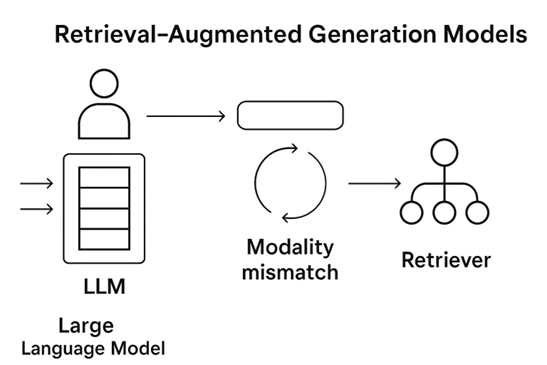
\includegraphics[width=0.72\linewidth]{figures/Picture4.png}
    \caption{Training flow and gating control in DLI-LLM. Product-quantized key--value lookup, attention fusion, routing gates, and gradient-based memory adaptation interact across Transformer blocks.}
    \label{fig:gating-control}
\end{figure}

\subsection{Toward Cognitive-Complete Transformer Architectures}
DLI-LLM argues for reconsidering memory-augmented Transformers not as storage-bound enhancements, but as components of a broader approach to machine cognition. In this view, retrieval is not merely a way to extend context length; it is a candidate mechanism for internal evidence selection, representational persistence, and adaptive control \cite{Anderson2007}. This aligns with the broader desideratum that cognitive architectures should integrate memory, learning, representation, and control into a coherent system \cite{Sun2004}.

\chapter{Volume I Conclusion}
Differentiable Latent Indexing proposes that retrieval can be moved from the periphery of language-model architecture into the differentiable interior of Transformer computation. The framework introduced here formalizes this idea through latent key--value memory, query projection, sparse retrieval, gated fusion, and a conceptual training objective. It also defines falsifiable propositions, expected benefits, and plausible failure modes.

The paper does not claim that DLI-LLM has already been implemented or empirically validated. Its contribution is theoretical: it clarifies what such an architecture would require, how it differs from existing retrieval and memory-augmented models, and what future experiments would need to test. As the first volume in the \textit{Latent Cognition Trilogy}, this article establishes memory as the initial boundary condition for a broader investigation into artificial cognition. % Volume I: Memory Fields (DLI) -> Starts at Page 1

\volumetitlepage
{Volume II: Symbol Fields}
{Curriculum-Induced Symbol Invention for Emergent Reasoning Primitives}
%%%%%%%%%%%%%%%%%%%%%%%%%%%%%%%%%%%%%%%%%%%%
%-------------------------------------------
\chapter*{Abstract}

This article introduces \textit{Curriculum-Induced Symbol Invention} (CISI), a theoretical framework for examining how discrete reasoning primitives may emerge within the intermediate representational pathways of Large Language Models (LLMs). Standard Transformer architectures operate primarily over continuous hidden states, and while these states may support complex behavior, the mechanisms by which recurring computational patterns stabilize into reusable abstractions remain only partially formalized. CISI proposes an architectural modification in which hidden-state trajectories are intercepted and compressed through an auxiliary vector-quantized latent codebook layer during pre-training.

Driven by a staged curriculum of increasing task complexity and an informational bottleneck, the model is pressured to stabilize and reuse internal codewords that function as compact computational primitives. In this sense, CISI treats symbol formation not as a post hoc linguistic mapping, but as a structural response to compression, reuse, and representational economy.

Building upon the internalized memory substrate established in \textit{Volume I: Memory Fields}, this work shifts the focus from continuous storage and retrieval to discrete abstraction. It provides a self-contained theoretical specification, including training stages, codebook optimization dynamics, semiographic translation probes, formal propositions, falsification conditions, and empirical evaluation protocols for the study of semiotics.

\noindent \textit{Keywords: Curriculum-Induced Symbol Invention (CISI); Latent Semiography; Vector Quantization; Information Bottleneck; Domain-Specific Languages; Machine Cognition; Structural Representation Learning; Automated Abstraction.}

%%%%%%%%%%%%%%%%%%%%%%%%%%%%%%%%%%%%%%%%%%%%
%==========================================
\section*{Position within the Research Program}

This manuscript constitutes \textbf{Volume} II of \textit{The Latent Cognition Trilogy}. It develops the symbolic abstraction layer of the broader research program by formalizing \textit{Curriculum-Induced Symbol Invention} (CISI) as a candidate mechanism through which compressed latent representations may acquire symbolic stability.

Volume I, \textit{Memory Fields}, established the memory layer of the Trilogy by treating retrieval as a native operation over latent representational structure. \textbf{Volume II} shifts the focus from memory access to symbolic compression. Its central claim is that, under curriculum pressure and representational bottlenecks, neural systems may stabilize reusable internal primitives that function as machine-generated symbolic structures.

The architectural foundation for the broader program remains \textit{Differentiable Latent Indexing in LLMs: Toward Native Retrieval as a Cognitive Function}. That work supplies the retrieval-native substrate. The present volume extends the sequence by asking how retrieved, compressed, and reused latent structures may become symbolically stable.

Accordingly, \textbf{Volume II} should not be read as a companion hypothesis paper. It is the second movement of the Trilogy. The companion hypothesis papers occupy a separate role: they isolate supporting claims without replacing the main sequence.

\chapter{Symbol Fields and Curriculum-Induced Symbol Invention}
\section{Introduction}
Volume II of \textit{The Latent Cognition Trilogy} examines the transition from latent memory to symbolic stabilization. Volume I established memory as a structured field of retrievable latent representations. The present volume asks a different question: under what conditions can compressed internal representations acquire sufficient stability, reusability, and functional specificity to serve as symbolic primitives within a neural architecture?
The central construct introduced here is \textit{Curriculum-Induced Symbol Invention} (CISI). CISI proposes that symbolic structure need not be imposed externally through hand-coded rules, symbolic grammars, or explicit logical systems. Instead, symbolic-like structures may emerge when a model is forced to solve increasingly complex tasks through a constrained intermediate representational bottleneck. Under such conditions, recurring computational patterns may be compressed into reusable latent codewords that function as internal abstractions.
The argument is not that large language models already possess explicit symbolic languages in the classical sense. Nor does CISI claim that vector quantization alone produces reasoning. The claim is narrower: a discrete intermediate codebook, trained under curriculum pressure and evaluated through stability, reuse, and transfer diagnostics, may provide a mechanism for studying how latent representations become symbolically organized.
Rather than viewing token tracking as an optimization task, Volume II addresses the classic Symbol Grounding Problem (Harnad, 1990) by observing sign evolution under physical architectural constraints. By forcing continuous states through a discrete vector-quantized bottleneck (van den Oord et al., 2017) governed by the Information Bottleneck Principle (Tishby et al., 2000), the network cannot remain passive. It must construct an explicit internal sign paradigm, validating the triadic semiotic structures hypothesized by Peirce (1931)
\section{Problem Space: From Continuous Representation to Symbolic Stability}
Transformer-based language models operate over high-dimensional continuous hidden states. These states support complex linguistic and reasoning behaviors, but their internal organization often remains difficult to characterize. A hidden state may simultaneously encode context, syntax, semantic associations, task-relevant features, and transient computational dynamics. This expressive richness creates a problem for symbolic interpretation: the model may behave as though it has reusable abstractions without exposing clear internal units corresponding to those abstractions.
Classical symbolic systems rely on discrete, composable, and reusable primitives. Neural systems, by contrast, distribute information across continuous representations. The challenge is therefore not simply to recover symbols from neural states, but to determine whether neural architectures can be pressured to form stable intermediate structures that play a symbol-like role without abandoning differentiable learning.
CISI addresses this problem by introducing three constraints. First, the model is trained under a staged curriculum that progressively increases compositional complexity. Second, an intermediate vector-quantized bottleneck prevents all information from passing through unconstrained continuous channels. Third, diagnostic probes evaluate whether discrete codewords become stable, reusable, and predictive of downstream reasoning operations.
Within this framework, symbolic stability is defined operationally rather than metaphysically. A latent codeword becomes symbolically relevant only if it satisfies three conditions: it is selected repeatedly across related contexts, it contributes measurably to task performance, and its functional role remains sufficiently stable across curriculum stages and out-of-distribution evaluations.
\section{Contributions}
This volume contributes the following elements:
\begin{enumerate}
    \item a theoretical framework for studying symbolic stabilization under curriculum pressure and representational compression;
    \item a vector-quantized bottleneck mechanism for forcing intermediate latent states into discrete reusable codewords;
    \item a full CISI training objective that combines language modeling, vector quantization, commitment, entropy regulation, reuse pressure, and symbolic stability;
    \item diagnostic metrics for codebook utilization, reuse concentration, symbolic drift, and codeword stability;
    \item a staged curriculum design intended to induce primitive, compositional, and integrative symbolic behavior;
    \item a semiographic probing framework for translating latent codeword activations into interpretable operational roles; and
    \item a set of failure modes and falsification conditions for distinguishing genuine symbolic stabilization from arbitrary discretization.
\end{enumerate}
\section{Overview of the Volume}
The remainder of this volume proceeds as follows. The next chapter defines the core propositions and falsification conditions for CISI. The following chapter develops the informational bottleneck and vector quantization mechanism. Subsequent chapters introduce the full CISI objective, codebook diagnostics, staged curriculum design, semiographic interpretation, failure modes, empirical evaluation protocols, and the relationship between symbolic stabilization and the routing mechanisms developed in Volume III.

\chapter{Related Work}
\section{Discrete Latent Representations}
CISI is closely related to research on discrete latent representation learning. Vector-quantized latent models demonstrate that continuous inputs can be mapped into learned discrete codebooks while preserving differentiability through surrogate gradient mechanisms \cite{VanDenOord2017}. This provides an important precedent for the CISI bottleneck: the architecture does not merely compress representations, but forces them to pass through a finite set of reusable latent units.
However, CISI differs from standard vector-quantized representation learning in its intended role. The codebook is not treated only as a compression device or generative modeling component. It is treated as a candidate substrate for symbolic stabilization, where codeword reuse, curriculum exposure, and downstream reasoning performance jointly determine whether a codeword has acquired functional symbolic value.
\section{Information Bottleneck and Compression}
The information bottleneck framework provides a theoretical basis for treating compression as a mechanism for extracting task-relevant structure \cite{Tishby2000}. In CISI, the bottleneck is not only informational but semiotic: it pressures the model to preserve useful computational distinctions while discarding irrelevant representational variation. A successful CISI codebook should therefore retain information needed for reasoning while reducing dependence on unconstrained continuous state propagation.
This distinction is important because not all compression is symbolic. A representation may be compressed while remaining uninterpretable, unstable, or task-specific. CISI therefore requires additional diagnostics for reuse, stability, and transfer beyond reconstruction error alone.
\section{Curriculum Learning and Compositional Generalization}
Curriculum learning suggests that training order can shape the acquisition of increasingly complex behaviors \cite{Bengio2009}. CISI adopts this principle by exposing the model to progressively structured tasks: primitive operations, compositional routines, and integrative reasoning contexts. The curriculum is not merely a training convenience. It functions as the developmental pressure under which reusable internal codewords may become stabilized.
This connects CISI to the broader problem of compositional generalization. Studies of systematic generalization show that neural models may struggle to transfer learned operations compositionally when training distributions do not force reusable abstractions \cite{Lake2018}. CISI addresses this limitation by treating compositional transfer as a test of whether latent codewords have become functionally reusable rather than locally memorized.
\section{Emergent Communication and Latent Semiotics}
Research on emergent communication shows that agents can develop task-specific signaling systems under pressure for coordination and efficiency \cite{Foerster2016}. CISI adapts this insight to the internal dynamics of a single model. Instead of agents communicating with one another, intermediate layers communicate through a constrained latent codebook. The resulting codewords may be interpreted as a form of internal semiography: a machine-generated representational scheme optimized for task performance rather than human readability.
This analogy must be used carefully. CISI does not assume that codewords are linguistic symbols. It treats them as operational primitives whose symbolic status must be earned through stability, reuse, transfer, and interpretability tests.
\section{Probing and Interpretability}
The interpretability of internal representations remains an open challenge in large language models. Probing studies attempt to identify what linguistic, semantic, or structural information is encoded in learned representations \cite{Rogers2020}. CISI extends this approach by making the intermediate representational substrate partially discrete. This may improve inspectability, but it also introduces a risk: discrete codewords can invite overinterpretation.
For this reason, CISI does not equate probe labels with symbol meaning. A codeword is not considered symbolic simply because a probe can attach a human-readable label to it. The label must remain stable across contexts, correspond to measurable functional effects, and survive ablation tests that demonstrate its contribution to downstream reasoning.



\vspace{2em}
\hrule
\vspace{2em}

\chapter{Propositions and Falsification Conditions}

The validity of Curriculum-Induced Symbol Invention as a theoretical mechanism rests upon explicit, predictable behavioral deviations from standard Transformer baselines. The following formal propositions establish the empirical boundaries of the architecture and dictate clear falsification parameters.

\section*{Proposition 1: Symbolic Abstraction Efficiency}
As structural curriculum complexity scales, an LLM computational graph constrained by a discrete intermediate vector-quantization bottleneck will demonstrate significantly greater cross-domain generalization and sample efficiency on out-of-distribution (OOD) reasoning tasks than standard continuous-state architectures with equivalent parameter density.

\textbf{Falsification Condition:} If a continuous-state baseline matches or exceeds the CISI architecture on downstream multi-step reasoning evaluations when controlled for training token exposure and active parameter count, the claim that discrete intermediate symbol coining resolves structural compositionality is falsified.

\section*{Proposition 2: Codebook Reuse and Structural Sparsity}
The optimization trajectory of a bounded latent codebook operating under variable curriculum demands will favor stabilizing a minimal, highly reusable set of primitive codewords over a strategy of continuous, uniform expansion of codebook resources.

\textbf{Falsification Condition:} If tracking codebook utilization profiles reveals a linear growth path proportional to task variation, or if the codebook selection entropy approaches maximum uniform distribution without distinct topological clustering, the hypothesis that the informational bottleneck forces symbolic compression is ungrounded.

\section*{Proposition 3: Degradation under Bottleneck Deactivation}
The deactivation or continuous relaxation of the intermediate quantization layer following curriculum exposure will result in a catastrophic degradation of out-of-distribution reasoning capabilities, while local in-distribution language modeling performance remains unaffected.

\textbf{Falsification Condition:} If an operational CISI model maintains its advanced multi-step reasoning capabilities when the vector quantization layer is bypassed or replaced with an unconstrained linear projection, the symbolic utility of the discrete codebook is disproven.

\chapter{The Informational Bottleneck and Vector Quantization}

Let $h_t^{(\ell)} \in \mathbb{R}^{d}$ define the continuous hidden representation of a token at sequence position $t$ and intermediate layer $\ell$ within the standard Transformer forward pass. The CISI architecture systematically intercepts this trajectory, passing the continuous vector field through a discrete quantization bottleneck before it propagates to subsequent layers.

\section{Vector Quantization Mechanics}
We define an internal, learned discrete codebook dictionary $\mathcal{C} = \{e_1, e_2, \dots, e_K\}$, where each individual codeword vector $e_k \in \mathbb{R}^{d}$. The continuous latent state $h_t^{(\ell)}$ is mapped directly to its nearest symbolic primitive within the dictionary via a minimum Euclidean distance projection operator:

\begin{equation}
z_t^{(\ell)} = \operatorname{vquant}\left(h_t^{(\ell)}\right) = e_{\hat{k}}, \quad \text{where } \hat{k} = \arg\min_{k} \|h_t^{(\ell)} - e_k\|_2.
\end{equation}

The selected codebook index $\hat{k}$ serves as the discrete, organic latent symbol invented by the architecture to represent that particular continuous computational sub-manifold.

\section{The Compression Objective}
To enforce intense compression pressure and protect the network against representational collapse or passive passing-through of uncompressed tokens, an auxiliary decoder head $\mathcal{D}$ is introduced. This decoder is tasked with reconstructing the complete, high-dimensional continuous hidden state $h_t^{(\ell)}$ using the quantized discrete vector assignment $z_t^{(\ell)}$:

\begin{equation}
\mathcal{L}_{\text{comp}} = \| \mathcal{D}\left(z_t^{(\ell)}\right) - \operatorname{sg}[h_t^{(\ell)}] \|_2^2 + \beta \| \operatorname{sg}[h_t^{(\ell)}] - z_t^{(\ell)} \|_2^2,
\end{equation}

where $\operatorname{sg}[\cdot]$ represents the classic stop-gradient operator required to prevent unstable backward oscillations during joint optimization, and $\beta$ is a commitment hyperparameter regulating the alignment rate between continuous trajectories and codebook coordinates.

\section{Full CISI Training Objective}

The vector-quantized bottleneck alone does not define the full CISI training process. It specifies how continuous hidden states are discretized, but the broader architecture requires an objective that jointly optimizes language modeling, codebook commitment, symbolic reuse, sparsity, and stability under curriculum pressure. A conceptual CISI objective can be written as:

\begin{equation}
\mathcal{L}_{CISI}
=
\mathcal{L}_{LM}
+
\lambda_q \mathcal{L}_{VQ}
+
\lambda_c \mathcal{L}_{commit}
+
\lambda_e \mathcal{L}_{entropy}
+
\lambda_r \mathcal{L}_{reuse}
+
\lambda_s \mathcal{L}_{stability}.
\end{equation}

Here, $\mathcal{L}_{LM}$ denotes the standard language modeling objective. The term $\mathcal{L}_{VQ}$ captures reconstruction error through the vector-quantized bottleneck, while $\mathcal{L}_{commit}$ encourages continuous hidden states to remain close to their assigned codebook vectors. The entropy term $\mathcal{L}_{entropy}$ regulates the distribution of codeword usage, preventing uncontrolled uniform expansion or premature collapse into a small number of dominant codes. The reuse term $\mathcal{L}_{reuse}$ encourages frequently useful codewords to persist across related tasks, while $\mathcal{L}_{stability}$ penalizes excessive drift in codeword meaning across curriculum stages.

The purpose of this objective is not merely to discretize hidden states. Its purpose is to create pressure for reusable symbolic structure. Under this formulation, a codeword becomes symbolically meaningful only if it is repeatedly selected, functionally useful, stable across related contexts, and predictive of downstream reasoning behavior.

\section{Codebook Diagnostics and Symbolic Stability}

The emergence of symbolic structure cannot be inferred from codebook discreteness alone. A vector-quantized layer may produce discrete indices without producing meaningful symbolic primitives. CISI therefore requires diagnostic criteria for distinguishing genuine symbolic stabilization from arbitrary quantization.

Let $p(e_k)$ denote the empirical activation frequency of codeword $e_k$ over a validation corpus. Codebook utilization entropy may be defined as:

\begin{equation}
H(\mathcal{C}) = - \sum_{k=1}^{K} p(e_k)\log p(e_k).
\end{equation}

A maximally uniform distribution may indicate insufficient specialization, while extreme concentration may indicate codebook collapse. Symbolic stabilization is expected to occur in an intermediate regime where a subset of codewords becomes highly reusable without eliminating functional diversity.

A reuse concentration score can be expressed as:

\begin{equation}
R(\mathcal{C}) = \sum_{k=1}^{K} p(e_k)^2.
\end{equation}

Higher values of $R(\mathcal{C})$ indicate repeated reliance on a smaller set of codewords, but this metric must be interpreted jointly with task performance and out-of-distribution generalization. Reuse alone is not sufficient evidence of symbolic structure; the reused codewords must also correspond to stable computational roles.

To evaluate stability across curriculum stages, let $p_t(e_k)$ and $p_{t+1}(e_k)$ denote codeword activation distributions at successive stages. A symbolic drift measure may be written as:

\begin{equation}
D_{symbol}(t,t+1) =
D_{KL}\left(p_t(e_k) \parallel p_{t+1}(e_k)\right).
\end{equation}

A stable symbolic codebook should exhibit decreasing drift after curriculum convergence, while still preserving enough plasticity to adapt to higher-order compositional tasks.

\chapter{Staged Curriculum Design}

The autonomous invention of logical primitives cannot successfully execute within unstructured, high-entropy text environments. It requires an evolutionary gradient. The CISI training framework uses a multi-tiered curriculum that systematically triggers symbol creation by varying operational complexity.

\begin{table}[h]
\centering
\small
\begin{tabular}{p{0.20\linewidth}p{0.36\linewidth}p{0.36\linewidth}}
\hline
\textbf{Curriculum Stage} & \textbf{Operational Complexity} & \textbf{Expected Symbolic Emergence} \\
\hline
\textbf{Stage 1: Primitives} & Single-digit arithmetic, basic relational logic statements, atomic parsing scripts. & Coining of baseline primitives (e.g., latent equivalents to functional terms like "ADD", "COMPARE"). \\
\textbf{Stage 2: Composition} & Compound functional routines, multi-hop dependencies, variable tracking loops. & Combination of Stage 1 codewords into complex, integrated computational blocks. \\
\textbf{Stage 3: Integration} & Knowledge-intensive text, open-domain reasoning benchmarks (GSM8K, CommonsenseQA). & Synthesis of a robust, highly optimized internal Domain-Specific Language (DSL). \\
\hline
\end{tabular}
\caption{The CISI Staged Training Curriculum Profile.}
\label{tab:cisi-curriculum}
\end{table}

During Stage 1, a minimal partition of $10$ to $20$ active codewords suffices for error minimization. As the model transitions to Stages 2 and 3, the codebook is permitted to expand under strict sparsity regularizers, thereby forcing previous symbols to act as structural building blocks for higher-order reasoning routines.

\chapter{Semiographic Projection and Interpretation}

Once symbols stabilize within the intermediate codebook substrate, they must be rendered inspectable to ensure cognitive accountability and alignment. CISI avoids back-correcting the network via human prose; instead, it reads the machine's internal language directly.

\section{Linear Probing and Linguistic Translation}
We introduce a periodic probing schedule using linear classification models applied directly to index activation frequencies over standardized validation partitions:

\begin{equation}
P(T_m \mid e_{\hat{k}}) = \operatorname{softmax}\left(W_p e_{\hat{k}} + b_p\right),
\end{equation}

where $T_m$ represents a human-interpretable linguistic concept or operational token. This translation layer functions as a forensic tool, decoding raw latent cluster identifiers into legible intermediate reasoning trajectories, thereby exposing the inner paths of the machine's deductive logic.

\chapter{Expected Failure Modes}
CISI is a theoretical mechanism, not a guaranteed path to symbolic reasoning. Its value depends on whether the proposed bottleneck and curriculum pressures produce stable, reusable, and functionally relevant codewords. Several failure modes must therefore be considered explicitly.
\section{Codebook Collapse}
The most direct failure mode is codebook collapse. In this case, the model relies on a small number of dominant codewords regardless of task variation. Although such collapse may appear efficient, it would indicate that the bottleneck has failed to preserve meaningful distinctions among computational operations. Collapse can be detected through low codebook entropy, high reuse concentration, and degraded out-of-distribution performance.
\section{Symbol Fragmentation}
The opposite failure mode is symbol fragmentation. Here, the model creates too many context-specific codewords, preventing reusable abstractions from forming. Fragmentation may yield high reconstruction accuracy while failing to support compositional transfer. A fragmented codebook behaves like a lookup table rather than a symbolic substrate.
\section{Pseudo-Symbol Formation}
A third failure mode is pseudo-symbol formation. The model may produce discrete codewords that appear stable under probing but do not causally contribute to reasoning performance. This failure can occur when probe classifiers identify superficial correlations rather than functional computational roles. Ablation tests are therefore necessary to determine whether codewords are operationally necessary.
\section{Curriculum Overfitting}
CISI depends on staged curriculum pressure. If the curriculum is too narrow, the model may invent codewords that are useful only for the training sequence and fail under distributional shift. Such overfitting would weaken the claim that the codebook captures reusable abstractions. The evaluation protocol must therefore include out-of-distribution and compositional transfer tasks.
\section{Probe-Induced Overinterpretation}
Semiographic projection introduces an interpretive risk. Human-readable labels assigned to codewords may suggest more structure than the model actually possesses. A codeword labeled as \textit{COMPARE}, for example, may not correspond to a stable comparison operation across contexts. CISI therefore treats probe labels as hypotheses, not explanations.
\section{Brittle Symbolic Transfer}
A CISI model may show improved performance on structured reasoning tasks while remaining brittle under mixed-domain, noisy, or adversarial inputs. This would suggest that symbolic stabilization has occurred only within a narrow operational regime. A robust symbolic field should preserve useful abstraction without becoming rigid or domain-bound.


\chapter{Empirical Evaluation Protocol}

To validate the theoretical assertions of Curriculum-Induced Symbol Invention, any experimental implementation must undergo a rigorous, multi-layered forensic protocol comprising four primary validation operations.

\section{Zero-Shot Out-of-Distribution Evaluation}
The primary benchmark for structural symbol creation is the model's ability to perform zero-shot transfer to entirely novel reasoning datasets. Following exposure to the staged curriculum, the CISI architecture must be evaluated on logic and relational datasets whose underlying semantic distributions share zero overlap with the training inputs. Performance metrics must be compared strictly against baseline Transformer models with identical parameter counts and token exposure.

\section{Ablation of the Compression Interface}
To prove that the discrete codebook is the active engine behind reasoning stability, developers must execute a structural ablation pass. By systematically disabling the compression layer post-training—or dynamically substituting the vector quantization operator with an unconstrained, continuous linear layer—the evaluator must track the exact delta in generalization performance. A corresponding drop in out-of-distribution accuracy confirms the operational necessity of the symbols.

\section{Topological Clustering and Code-Reuse Metrics}
The spatial distribution of the codebook must be mathematically evaluated using the localized Silhouette Coefficient ($S$) formalized in the canon of Volume I. Evaluators must verify that the continuous hidden states collapse into highly concentrated, discrete geometric regions surrounding active codebook centroids. Furthermore, the codebook utilization profile must exhibit a Power Law distribution, confirming high code reuse across disparate tasks.

\section{Human Semiotic Mapping and Consistency Studies}
Finally, the cognitive validity of the invented internal symbols must be tested through a blind human annotation study. Human evaluators are presented with isolated activation maps for specific codewords, alongside their corresponding linguistic contexts, decoded via the linear-probing translation matrix. Annotators are tasked with mapping these active indices to precise English descriptions or operational rules. The degree of semantic agreement among annotators is quantified using Fleiss' Kappa ($\kappa$), which verifies whether the machine's invented symbols correspond to stable, invariant concepts.

\chapter{Discussion}
\section{Cognitive Interpretation}
CISI reframes symbolic abstraction as a possible consequence of representational compression under structured training pressure. In this view, symbols are not assumed to be externally supplied units. They are treated as stabilized internal codes that emerge when the model must preserve reusable computational structure through a constrained channel.
This interpretation occupies a middle ground between continuous representation learning and classical symbolic reasoning. CISI does not reject distributed neural representation, but it argues that some forms of reasoning may require intermediate structures that are more stable, reusable, and inspectable than ordinary hidden states. The codebook provides one possible mechanism for producing such structures.
\section{Relation to Volume I}
Volume I established the memory layer of the Trilogy by treating retrieval as a native operation over latent representational fields. Volume II extends that argument by asking how retrieved or compressed latent structures may become symbolically stable. Memory supplies access to latent structure; symbolic stabilization supplies reusable abstraction.
The relation between DLI and CISI is therefore sequential but not strictly causal. A system may implement latent memory without symbolic stabilization, and it may implement a symbolic bottleneck without DLI. Within the Trilogy, however, the two mechanisms are treated as complementary layers of a broader latent cognitive architecture.
\section{Interpretability and Accountability}
The partial discreteness of CISI may improve interpretability by creating identifiable intermediate units. However, discreteness alone does not guarantee transparency. A codeword may be stable but uninterpretable, interpretable but non-causal, or causal only within narrow contexts. For this reason, CISI requires multiple forms of evidence: probing, ablation, transfer testing, entropy analysis, and human annotation.
This layered interpretability strategy is central to the framework. It prevents the model's invented codebook from being romanticized as a private language unless its operational role can be demonstrated.
\section{Limits of the Framework}
CISI does not prove that neural models can invent symbols in the strong philosophical sense. It defines a testable architectural pathway for studying symbol-like stabilization. The framework remains theoretical until implemented and compared against continuous-state baselines, vector-quantized controls, and curriculum-free alternatives.
The strongest version of CISI would be supported only if discrete codewords improve systematic generalization, remain stable across curriculum stages, survive ablation tests, and correspond to interpretable computational roles. Without such evidence, the framework should be treated as a useful compression architecture rather than a theory of machine symbol formation.
\chapter{Volume II Conclusion}
Volume II has developed \textit{Curriculum-Induced Symbol Invention} as the symbolic abstraction layer of \textit{The Latent Cognition Trilogy}. Its central claim is that symbolic stability may arise when continuous latent representations are forced through a discrete bottleneck under curriculum pressure and then reused across increasingly complex tasks.
The proposed framework does not equate discretization with symbolism. Instead, it defines symbolic relevance in terms of stability, reuse, functional contribution, and transfer. A codeword becomes symbolically meaningful only when it behaves as a reusable computational primitive rather than as an arbitrary index in a learned codebook.
CISI therefore contributes a theoretical bridge between latent memory and architectural routing. Volume I described how memory may be treated as an internal field of retrievable representations. Volume II has examined how such representations may become compressed into reusable abstractions. Volume III extends the sequence by asking how memory fields and symbol fields can be coordinated through hierarchical routing mechanisms across distributed neural architectures.
\section{Transition to Volume III}
Volume I establishes the memory layer of the Trilogy. Volume II examines how compressed latent states may acquire symbolic stability. Volume III will then analyze how memory and symbolic structures may be coordinated through hierarchical routing.


% \bibliographystyle{plain}
% \bibliography{references.bib}
 % Volume II: Symbolic Evolution

\volumetitlepagewithfig
{Volume III: Routing Fields}
{Hierarchical Topic-Conditioned Routing for Mixture-of-Expert Language Models}

\begin{figure}[h!]
\centering
% Top: Field + emerged symbol = CISI core claim

\begin{minipage}{0.75\textwidth}
    \centering
    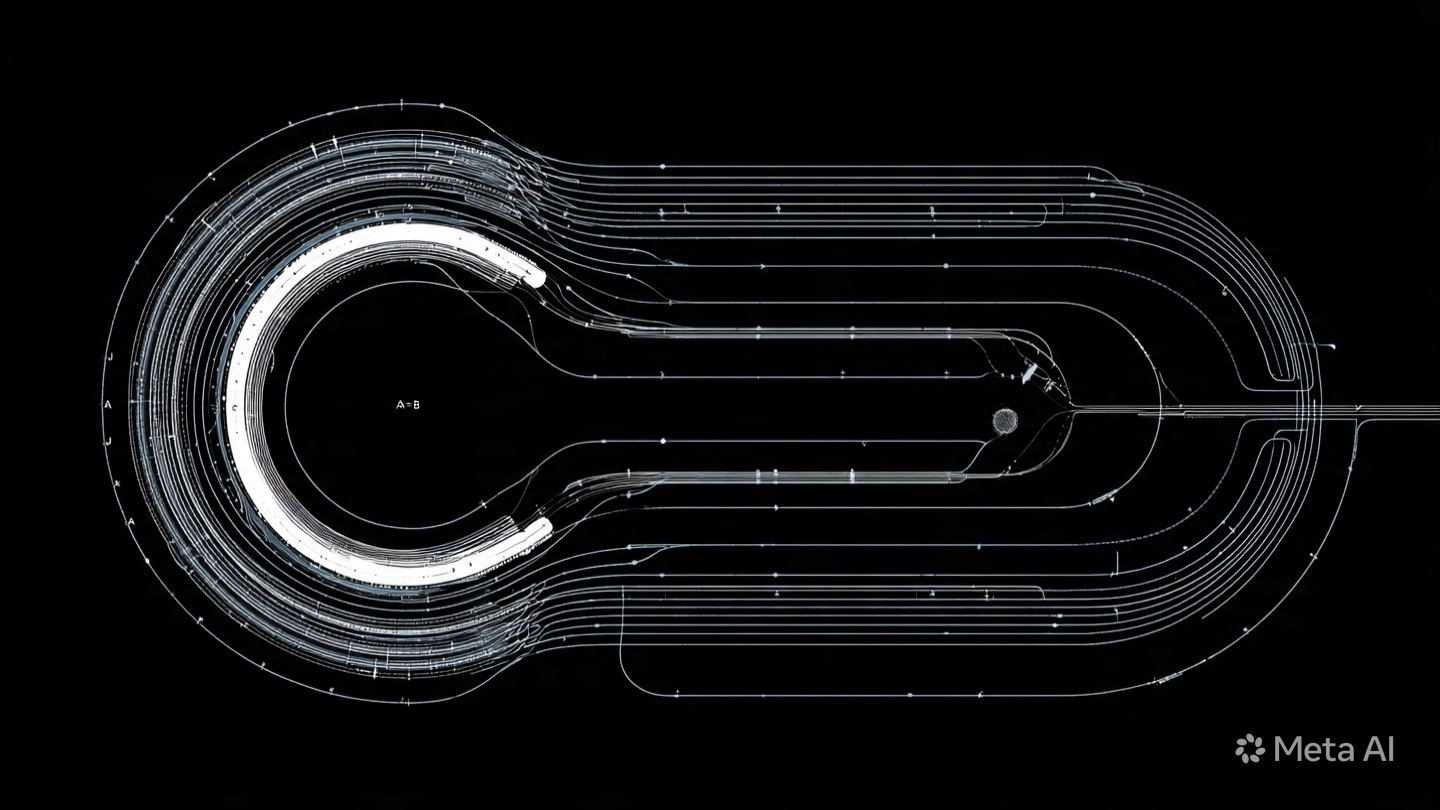
\includegraphics[width=\linewidth]{figures/image-vol3-covera.jpeg}
    % Option 2: Operator Signature
\end{minipage}

\vspace{0.8cm} % space between the two
% Bottom: Abstract VQ bottleneck

\begin{minipage}{0.75\textwidth}
    \centering
    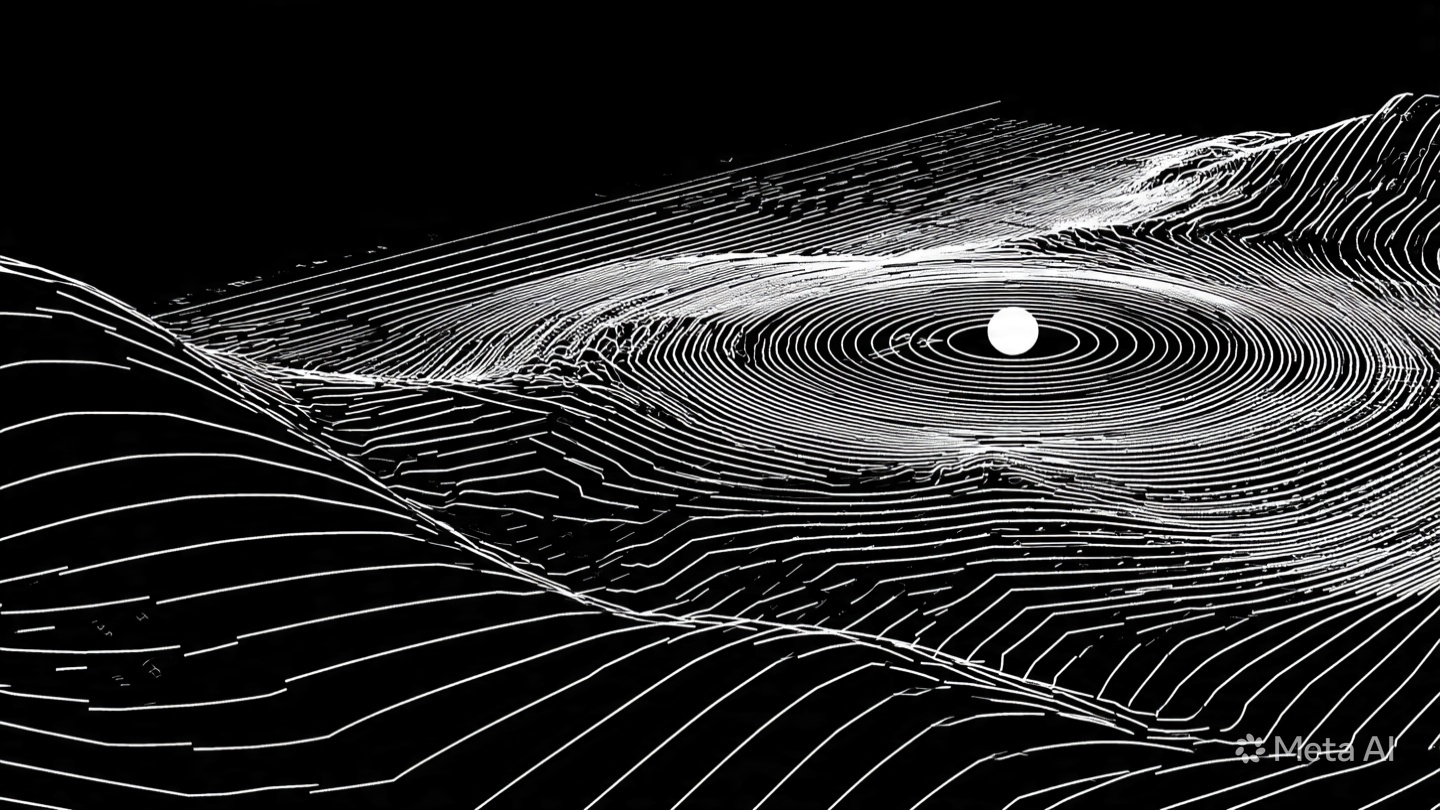
\includegraphics[width=\linewidth]{figures/image-vol3-coverb.jpeg}
    % Option 2: Operator Signature
\end{minipage}
\end{figure}
%%%%%%%%%%%%%%%%%%%%%%%%%%%%%%%%%%%%%%%
%======================================
\chapter*{Abstract}

This article introduces \textit{Hierarchical Topic-Conditioned Routing} (HTCR), an architectural framework for examining how routing mechanisms may improve coherence, cache locality, and computational organization within sparse Mixture-of-Experts (MoE) language models. Standard MoE architectures frequently rely on token-level routing decisions, which can fragment sequence-level structure and increase volatility in expert assignment during long-context inference. This token-local routing pattern may contribute to expert jitter, reduced cache reuse, and increased communication overhead in distributed execution environments.

HTCR proposes a two-tier routing mechanism. First, a macroscopic document- or segment-level router assigns local context segments of $N$ tokens to a restricted pool of $m$ candidate experts. Second, a microscopic token-level router dispatches individual tokens exclusively within that pre-allocated expert shortlist. This hierarchy is intended to preserve local semantic coherence while reducing unnecessary expert dispersion during long-sequence processing.

Building upon the memory substrates of \textit{Volume I: Memory Fields} and the symbolic abstractions of \textit{Volume II: Symbol Fields}, HTCR concludes the Trilogy by defining a dynamic macroscale routing infrastructure for distributed latent computation. This work provides a theoretical reference design, including mathematical mechanics for two-stage dispatch, structural load-balancing metrics, training stability regularizers, and empirical validation protocols for routing-aware neural architectures.

\noindent \textit{Keywords: Hierarchical Topic-Conditioned Routing (HTCR); Mixture-of-Experts (MoE); Cache Locality; Distributed Inference; Expert Jitter; Token Dispatch; Structural Regularization.}

\chapter{Routing Fields and Hierarchical Topic-Conditioned Routing}

\section{Introduction}

Volume III of \textit{The Latent Cognition Trilogy} examines the architectural coordination layer of latent cognition. Volume I developed memory as a field of retrievable latent representations. Volume II examined how compressed latent states may acquire symbolic stability under curriculum and bottleneck pressure. Volume III addresses the next structural question: how can memory fields and symbol fields be coordinated across large-scale neural architectures whose computation is distributed across specialized components?

The central construct introduced here is \textit{Hierarchical Topic-Conditioned Routing} (HTCR). HTCR proposes that routing should not be treated only as a token-local dispatch mechanism or a hardware efficiency optimization. Instead, routing may be understood as a structural principle through which computation is allocated, constrained, and stabilized across expert modules. In this framing, routing becomes the architectural mechanism that determines where latent information is processed, which expert pathways are activated, and how coherence is preserved across long sequences.

Standard sparse Mixture-of-Experts (MoE) systems often route tokens independently. This design allows conditional computation at scale, but it can fragment sequence-level structure, increase expert assignment volatility, and create communication patterns that are difficult to optimize in distributed inference. HTCR introduces a two-stage routing process: first, a segment-level router identifies a restricted expert pool for a local context region; second, a token-level router dispatches individual tokens only within that constrained pool.

The purpose of this volume is not to claim that HTCR has been empirically validated. Rather, it develops a theoretical and systems-oriented framework for evaluating whether hierarchical routing can reduce expert jitter, improve cache locality, stabilize load balancing, and preserve semantic coherence across long-context computation.

Standard mixture-of-expert models scale parameters by introducing structural disorder, optimizing gating functions at an isolated token level (Shazeer et al., 2017). This introduces token jitter and shatters context continuity. Grounded in Herbert Simon’s formulation of nearly-decomposable complex systems (Simon, 1996), we introduce Hierarchical Topic-Conditioned Routing (HTCR). By structuring expert allocation into a macro-scale context partition and a micro-scale token dispatch, we implement a stable multi-tier cognitive layout that mirrors the macro/micro cognitive constraints established in classical cognitive theory (Miller, 1956; Sun, 2004).

\section{Problem Space: Token-Level Routing and Architectural Fragmentation}

Sparse MoE models increase model capacity by activating only a subset of expert parameters for each token. This provides an attractive scaling strategy: the total parameter count may grow substantially while the active computation per token remains bounded. However, token-level routing also introduces a coordination problem. If each token independently selects experts, adjacent tokens in a semantically coherent passage may be dispatched to unstable or widely dispersed expert sets.

This token-local routing pattern can produce several difficulties. First, expert assignment may fluctuate rapidly across neighboring tokens, creating what this volume refers to as \textit{expert jitter}. Second, distributed execution may require expensive all-to-all communication when tokens in the same sequence are routed to experts located across different hardware partitions. Third, cache reuse may be weakened when expert activation patterns change too frequently across local context windows.

HTCR addresses these issues by adding a macroscopic routing stage before token-level dispatch. Instead of allowing every token to select from the full expert pool independently, the segment-level router selects a bounded shortlist of candidate experts for a local context segment. Token-level routing then proceeds within that shortlist. The hypothesis is that this hierarchical constraint may preserve semantic locality while reducing unnecessary routing dispersion.

Within the broader Trilogy, this problem has cognitive significance. Memory and symbolic abstraction are not sufficient unless the architecture can coordinate where and how they are processed. Routing therefore becomes the mechanism through which latent cognition is operationally organized across distributed computation.

\section{Contributions}

This volume contributes the following elements:

\begin{enumerate}
    \item a theoretical framework for interpreting routing as architectural coordination rather than only conditional computation;
    \item a two-stage HTCR mechanism combining macroscopic segment routing with microscopic token dispatch;
    \item formal metrics for expert jitter, shortlist stability, routing entropy, load balancing, and communication cost;
    \item a cache-locality analysis for long-context MoE inference;
    \item an empirical evaluation protocol for comparing HTCR against flat token-routed MoE baselines;
    \item a failure-mode taxonomy for hierarchical routing architectures; and
    \item a synthesis of routing as the third layer of the Trilogy's memory--symbol--routing sequence.
\end{enumerate}

\section{Overview of the Volume}

The remainder of this volume proceeds as follows. The next chapter situates HTCR within related work on sparse MoE architectures, token routing, load balancing, expert choice mechanisms, and long-context inference. Subsequent chapters define the propositions and falsification conditions, formalize the dual-stage routing mechanism, introduce stability and locality metrics, specify structural regularization terms, define expected failure modes, and outline empirical validation protocols.

%%%%%%%%%%%%%%%%%%%%%%%%%%%%%%%%%%%%%%%%%%%%%%%%%
%================================================
\section*{Position within the Research Program}

This manuscript constitutes \textbf{Volume III} of \textit{The Latent Cognition Trilogy}. It develops the routing and architectural coordination layer of the broader research program by formalizing \textit{Hierarchical Topic-Conditioned Routing} (HTCR) as a candidate mechanism for organizing distributed computation across specialized model components.

\textbf{Volume I}, \textit{Memory Fields}, established the memory layer of the Trilogy by treating retrieval as a native operation over latent representational structure. \textbf{Volume II}, \textit{Symbol Fields}, examined the conditions under which compressed latent representations may acquire symbolic stability. Volume III extends this sequence by asking how memory and symbolic structures may be coordinated across large-scale architectures through hierarchical routing mechanisms.

The architectural foundation for the broader program remains \textit{Differentiable Latent Indexing in LLMs: Toward Native Retrieval as a Cognitive Function}. That work supplies the retrieval-native substrate from which the Trilogy begins. The present volume completes the main sequence by shifting attention from memory and symbolic abstraction to the coordination of computation across expert modules, routing pathways, and distributed inference structures.

Accordingly, \textbf{Volume III} should not be read as a companion hypothesis paper. It is the third movement of the Trilogy. The companion hypothesis papers occupy a separate role: they isolate supporting claims without replacing the main sequence.

\chapter{Related Work}

\section{Sparse Mixture-of-Experts Models}

Sparse Mixture-of-Experts architectures provide the immediate technical context for HTCR. Sparsely-Gated MoE introduced the use of trainable gating networks to route inputs to a sparse subset of expert feed-forward networks, enabling large increases in model capacity without activating all parameters for every input \cite{Shazeer2017}. GShard extended this direction by combining conditional computation with automatic sharding, making large-scale sparse expert models more practical in distributed settings \cite{Lepikhin2020}.

HTCR builds on this lineage but shifts the focus from capacity scaling to routing coherence. The central question is not simply whether sparse experts can increase model size efficiently, but whether routing can preserve sequence-level structure and reduce expert volatility during long-context processing.

\section{Routing Simplification and Load Balancing}

Switch Transformer simplified MoE routing by selecting a single expert per token and introduced techniques for improving stability and reducing communication overhead \cite{Fedus2022}. ST-MoE further examined stability and transferability in sparse expert models, emphasizing the practical difficulty of training sparse systems that remain reliable across tasks \cite{Zoph2022}.

These works motivate HTCR's concern with balancing. A routing mechanism must avoid expert starvation, token dropping, and pathological concentration of traffic into a small number of experts. HTCR therefore includes macro-level entropy regularization and load-balancing penalties, but adds a further constraint: balancing should occur without destroying local semantic coherence.

\section{Large-Scale Sparse Language Models}

GLaM demonstrated that sparsely activated MoE language models can scale model capacity while reducing training and inference cost relative to dense alternatives \cite{Du2022}. Mixtral later provided a modern sparse MoE language model in which each token is routed to a small subset of experts at each layer \cite{Jiang2024}. These systems show the practical relevance of sparse expert routing for language modeling at scale.

HTCR differs from these systems by introducing segment-conditioned expert shortlists. Rather than allowing every token to route against the full expert pool independently, HTCR constrains token-level routing through a local context-conditioned expert set.

\section{Alternative Routing Mechanisms}

Expert Choice Routing reverses the usual token-choice pattern by allowing experts to select tokens rather than requiring each token to select a fixed number of experts \cite{Zhou2022}. This approach directly addresses load imbalance and expert underutilization. HTCR is compatible with this broader design space because it also challenges unconstrained token-local routing, but it does so through hierarchical context conditioning rather than expert-side token selection.

The relevance of Expert Choice Routing for HTCR is conceptual as much as technical: routing policy is not a fixed implementation detail. It is an architectural design axis that can alter training dynamics, load distribution, specialization, and inference behavior.

\section{Distributed MoE Training and Hardware Efficiency}

Efficient sparse training requires alignment between routing dynamics and hardware execution. MegaBlocks reformulates MoE computation using block-sparse operations to avoid token dropping and reduce the mismatch between dynamic routing and GPU efficiency \cite{Gale2023}. This line of work shows that routing is not only a modeling question; it is also a systems problem involving memory layout, communication, batching, and kernel efficiency.

HTCR extends this systems concern to long-context inference. If semantically related tokens can be routed through a more stable local expert pool, the resulting execution pattern may improve cache locality and reduce unnecessary all-to-all expert movement.

\section{Long-Context Inference and KV-Cache Locality}

Long-context inference introduces significant memory-management pressure because key--value cache size grows with sequence length. PagedAttention and vLLM address this problem by managing KV cache through paged memory structures, improving serving throughput and reducing memory waste \cite{Kwon2023}. Although HTCR does not replace cache-management systems, it targets an adjacent problem: the instability of expert activation patterns that can reduce locality in sparse expert inference.

The connection is therefore structural. KV-cache systems manage memory efficiently once computation is scheduled. HTCR attempts to make the computation schedule itself more locality-preserving by reducing expert dispersion within semantically coherent segments.

\vspace{2em}
\hrule
\vspace{2em}

\chapter{Propositions and Falsification Conditions}

The validity of Hierarchical Topic-Conditioned Routing as a theoretical routing mechanism rests on verifiable behavioral differences relative to flat token-routed MoE baselines (such as standard Mixtral or GShard configurations).

\section*{Proposition 1: Topological Cache Locality and Throughput}
By constraining individual token execution trajectories to a segment-bounded expert shortlist, the HTCR framework will demonstrate a significant reduction in inter-device KV cache communication volume and yield higher token-processing throughput during long-context sequence execution.

\textbf{Falsification Condition:} If an HTCR model manifests equivalent or higher inter-node communication latency and lower generation throughput compared to an unconstrained token-MoE baseline when evaluated on continuous context lengths exceeding $32\text{k}$ tokens, the utility of segment-level clustering is falsified.

\section*{Proposition 2: Optimization Stability and Load Balancing}
The combination of macro-level entropy regularizers and token-level gates will stabilize expert assignment trajectories, preventing severe expert starvation and balancing computational loads across distributed hardware partitions without sacrificing modeling capacity.

\textbf{Falsification Condition:} If tracking routing distributions during large-scale pre-training reveals persistent structural load imbalances, or if token-drop ratios match flat gating methods under maximum hardware throughput limits, the optimization balancing claims are ungrounded.

\chapter{The Dual-Stage Hierarchical Routing Architecture}

Let a long-context sequence be partitioned into discrete segments $S_j$ containing $N$ sequential tokens, where the input token matrix is defined as $X \in \mathbb{R}^{N \times d}$. 

\section{Stage 1: Macroscopic Segment Routing}
Before token-level evaluation begins, the local hidden representations from the previous layer are aggregated into a unified segment-level summary vector $s_j \in \mathbb{R}^{d}$ via strategic mean-pooling across the spatial dimension:

\begin{equation}
s_j = \frac{1}{N}\sum_{t=1}^{N} h_t^{(\ell-1)}.
\end{equation}

This summary vector $s_j$ is processed by a document-router $\mathcal{R}_{\text{doc}}$, parameterized by a two-layer Multi-Layer Perceptron (MLP), to compute an allocation profile over the entire pool of $E$ total available experts:

\begin{equation}
G_{\text{doc}}(s_j) = \operatorname{softmax}\left(W_2 \cdot \operatorname{GeLU}\left(W_1 s_j + b_1\right) + b_2\right).
\end{equation}

The top-$m$ indices matching the highest activation values in $G_{\text{doc}}(s_j)$ are extracted to define the restricted active expert shortlist $\mathcal{M}_j = \{i_1, i_2, \dots, i_m\}$ for the duration of segment $S_j$.

\section{Stage 2: Microscopic Token Dispatch}
For each individual token representation $h_t^{(\ell)}$ residing within segment $S_j$, the local token-router $\mathcal{R}_{\text{tok}}$ evaluates gating scores \textit{exclusively} against the experts preserved in the shortlist $\mathcal{M}_j$:

\begin{equation}
G_{\text{tok}}\left(h_t^{(\ell)}\right) = \operatorname{softmax}\left( \left\{ w_k^{\top} h_t^{(\ell)} \;\middle|\; k \in \mathcal{M}_j \right\} \right).
\end{equation}

Individual tokens are then dispatched to the top-$k$ experts selected strictly from this local dictionary. Gradients flow end-to-end through both routing layers simultaneously via continuous backpropagation paths.

\section{Routing Stability and Expert Locality Metrics}

The central claim of HTCR is not merely that routing occurs in two stages. Its claim is that hierarchical routing should produce measurably more stable expert assignment patterns than unconstrained token-level routing. This requires explicit metrics for routing stability, expert dispersion, and local semantic coherence.

Let $\mathcal{M}_j$ denote the expert shortlist assigned to segment $S_j$. A simple shortlist stability score between adjacent segments can be defined as the Jaccard overlap:

\begin{equation}
\rho_j =
\frac{|\mathcal{M}_j \cap \mathcal{M}_{j+1}|}
{|\mathcal{M}_j \cup \mathcal{M}_{j+1}|}.
\end{equation}

High values of $\rho_j$ indicate that adjacent segments preserve similar expert pools, while low values indicate abrupt routing shifts. In long-context processing, moderate stability is desirable: the routing pattern should remain coherent across semantically continuous segments while still adapting when the topic or task structure changes.

Expert jitter can be defined as the complement of average shortlist stability:

\begin{equation}
J_{\text{expert}} =
1 -
\frac{1}{J-1}
\sum_{j=1}^{J-1}
\rho_j.
\end{equation}

A successful HTCR model should reduce $J_{\text{expert}}$ relative to a flat token-routed MoE baseline, particularly on long documents with locally coherent semantic structure.

\section{Routing Entropy and Load Distribution}

Let $p_e$ denote the empirical probability that expert $e$ is selected by the macroscopic segment router across a batch or validation corpus. Macro-routing entropy can be defined as:

\begin{equation}
H_{\text{doc}} =
-\sum_{e=1}^{E} p_e \log p_e.
\end{equation}

Very low entropy indicates routing collapse, where the segment router repeatedly selects a small number of experts. Very high entropy may indicate insufficient specialization, where the router fails to form meaningful associations between segment structure and expert allocation. HTCR therefore seeks a controlled intermediate regime: enough diversity to prevent starvation, but enough structure to support specialization and locality.

Load deviation from a uniform target can be measured as:

\begin{equation}
\Delta_{\text{load}} =
D_{KL}\left(\bar{G}_{\text{doc}} \parallel \mathcal{U}\right),
\end{equation}

where $\bar{G}_{\text{doc}}$ is the average macro-routing distribution and $\mathcal{U}$ is a uniform distribution over the expert pool. This term also appears in the regularization objective and functions as a diagnostic measure during evaluation.

\section{Communication Cost Model}

In distributed MoE inference, routing decisions induce communication costs when tokens are dispatched to experts located on different devices. Let $c(e_a,e_b)$ denote the communication cost associated with moving activation or cache-relevant information between device partitions associated with experts $e_a$ and $e_b$. For a flat token-routed MoE baseline, the communication cost over a segment may be approximated as:

\begin{equation}
\mathcal{C}_{\text{flat}}(S_j)
=
\sum_{t \in S_j}
\sum_{e \in \mathcal{E}_t}
c(d_t, d_e),
\end{equation}

where $\mathcal{E}_t$ denotes the expert set selected for token $t$, $d_t$ denotes the current device location of the token representation, and $d_e$ denotes the device hosting expert $e$.

Under HTCR, token routing is constrained to the segment shortlist $\mathcal{M}_j$, producing:

\begin{equation}
\mathcal{C}_{\text{HTCR}}(S_j)
=
\sum_{t \in S_j}
\sum_{e \in \mathcal{E}_t \cap \mathcal{M}_j}
c(d_t, d_e).
\end{equation}

The expected systems advantage of HTCR can be expressed as:

\begin{equation}
\Delta_{\text{comm}}
=
\mathbb{E}_{S_j}
\left[
\mathcal{C}_{\text{flat}}(S_j)
-
\mathcal{C}_{\text{HTCR}}(S_j)
\right].
\end{equation}

A positive $\Delta_{\text{comm}}$ indicates that hierarchical routing reduces communication pressure relative to unconstrained token-level dispatch.

\section{Cache Locality Objective}

HTCR can also be evaluated through a cache-locality objective. Let $A_t$ denote the expert activation set for token $t$. For adjacent tokens within a segment, local expert continuity can be defined as:

\begin{equation}
L_{\text{cache}}(S_j)
=
\frac{1}{N-1}
\sum_{t=1}^{N-1}
\frac{|A_t \cap A_{t+1}|}
{|A_t \cup A_{t+1}|}.
\end{equation}

Higher values of $L_{\text{cache}}$ indicate that neighboring tokens reuse similar expert pathways, increasing the likelihood of improved cache behavior and reduced expert-switching overhead. This metric does not replace hardware-level cache profiling, but it provides a model-level proxy for routing locality.

\chapter{Algorithmic Specification}

To operationalize HTCR, Algorithm~\ref{alg:htcr-loop} defines a single hierarchical routing step for one segment within one MoE layer.

\begin{center}
\fbox{%
\begin{minipage}{0.92\linewidth}
\textbf{Algorithm 2}: Hierarchical Topic-Conditioned Routing Loop\label{alg:htcr-loop}

\textbf{Input:} segment hidden states $H_j^{(\ell-1)} = \{h_t^{(\ell-1)}\}_{t=1}^{N}$, expert pool $\mathcal{E}$, document router $\mathcal{R}_{doc}$, token router $\mathcal{R}_{tok}$, shortlist size $m$, token top-$k$ value.

\textbf{Output:} routed expert assignments for all tokens in segment $S_j$.

\begin{enumerate}
    \item Compute segment summary:
    \[
    s_j \leftarrow \frac{1}{N}\sum_{t=1}^{N} h_t^{(\ell-1)}.
    \]
    \item Compute macro-routing distribution:
    \[
    G_{\text{doc}}(s_j) \leftarrow \mathcal{R}_{doc}(s_j).
    \]
    \item Select segment expert shortlist:
    \[
    \mathcal{M}_j \leftarrow \operatorname{TopM}(G_{\text{doc}}(s_j),m).
    \]
    \item For each token $t \in S_j$, compute token routing scores only over $\mathcal{M}_j$.
    \item Select top-$k$ experts for each token from $\mathcal{M}_j$.
    \item Dispatch token representations to selected experts.
    \item Aggregate expert outputs and return routed segment representations.
\end{enumerate}
\end{minipage}}
\end{center}

This procedure differs from flat token-level MoE routing by constraining the local search space before token dispatch. The document router establishes a coarse semantic prior over expert selection, while the token router preserves fine-grained flexibility inside that prior.

\chapter{Structural Regularization and Starvation Prevention}

To prevent the macroscopic document-router from collapsing into a biased state where a subset of experts absorbs all workloads (starvation), we enforce an auxiliary balanced regularization penalty $\mathcal{L}_{\text{bal}}$ during pre-training:

\begin{equation}
\mathcal{L}_{\text{total}} = \mathcal{L}_{\text{task}} + \lambda_1 \mathcal{L}_{\text{entropy}} + \lambda_2 \mathcal{D}_{\text{KL}}\left(\bar{G}_{\text{doc}} \parallel \mathcal{U}\right),
\end{equation}

where $\bar{G}_{\text{doc}}$ is the average macro-routing distribution across the training batch, $\mathcal{U}$ represents a uniform distribution over the expert pool $E$, and hyperparameters $\lambda_1, \lambda_2$ govern the structural smoothing constraints. The shortlist ceiling parameter $m$ is dynamically annealed throughout training, starting wide to maximize early discovery and tightening progressively to optimize final execution speed.

\section{Full HTCR Training Objective}

The balancing penalty alone does not define the full HTCR training process. A complete conceptual objective must account for task performance, macro-router entropy, load balancing, cache locality, and excessive routing volatility. A general HTCR objective can be written as:

\begin{equation}
\mathcal{L}_{HTCR}
=
\mathcal{L}_{task}
+
\lambda_b \mathcal{L}_{balance}
+
\lambda_h \mathcal{L}_{entropy}
+
\lambda_j \mathcal{L}_{jitter}
+
\lambda_l \mathcal{L}_{locality}.
\end{equation}

Here, $\mathcal{L}_{task}$ is the standard language modeling or downstream task objective. The term $\mathcal{L}_{balance}$ penalizes expert starvation or excessive load concentration. The entropy term $\mathcal{L}_{entropy}$ regulates the macro-router's selection profile. The jitter penalty $\mathcal{L}_{jitter}$ discourages unnecessary expert-set volatility across adjacent segments, while $\mathcal{L}_{locality}$ rewards stable expert reuse within semantically coherent regions.

The objective should not force all neighboring segments to use the same experts. Such rigidity would prevent adaptation to topic shifts. Instead, the goal is controlled continuity: stable routing when the local semantic structure is stable, and flexible rerouting when the segment content changes.

\section{Shortlist Annealing}

The shortlist ceiling parameter $m$ may be dynamically annealed during training. Early in training, a larger value of $m$ allows the model to explore a broader region of the expert pool. As training progresses, $m$ can be reduced to encourage sharper specialization and lower communication overhead.

This annealing schedule creates a trade-off between exploration and locality. If $m$ remains too large, HTCR degenerates toward flat token routing. If $m$ becomes too small too early, the model may overcommit to unstable expert assignments and prevent useful specialization from emerging. The annealing path must therefore be treated as a tunable systems parameter rather than a fixed architectural constant.

\chapter{Expected Failure Modes}

HTCR is a theoretical routing mechanism. Its value depends on whether hierarchical routing improves coherence, locality, and load balance without reducing modeling capacity. Several failure modes must therefore be evaluated explicitly.

\section{Topic Collapse}

The macroscopic segment router may collapse into selecting the same small expert subset for many unrelated segments. This would reduce communication volatility but destroy specialization. Topic collapse can be detected through low macro-routing entropy, poor expert diversity, and degraded performance on heterogeneous documents.

\section{Routing Inertia}

The opposite failure mode is excessive routing inertia. In this case, the segment router continues using the same expert shortlist even after the semantic structure of the document changes. Routing inertia may improve cache locality while harming adaptation. This failure is especially likely in documents with abrupt topic shifts, code-switching, multi-domain reasoning, or mixed-format inputs.

\section{Segment-Boundary Error}

HTCR depends on segment partitioning. If segment boundaries cut across coherent semantic units, the macro-router may assign inappropriate expert pools. Boundary errors may occur in long documents where topic transitions do not align with fixed token windows. Adaptive segmentation may therefore be required in future implementations.

\section{Expert Starvation}

Despite balancing penalties, some experts may remain undertrained if the segment router repeatedly excludes them from shortlists. Expert starvation can reduce the effective capacity of the model and may produce brittle specialization. Evaluation must track not only token-level load but also macro-level shortlist inclusion frequency.

\section{Over-Specialized Experts}

HTCR may encourage experts to specialize too narrowly around segment categories. Such over-specialization may improve local performance while weakening generalization. This failure can be detected when expert-specific performance becomes highly domain-bound and transfer across related tasks declines.

\section{Communication Overhead from Macro-Routing}

The additional document-router stage may introduce overhead that outweighs the savings from reduced token-level dispersion. This would falsify the systems-efficiency motivation for HTCR. A fair evaluation must therefore include end-to-end latency, throughput, memory movement, and scheduling overhead, not only theoretical communication counts.

\section{Reduced Flexibility under Mixed-Topic Contexts}

A restricted expert shortlist may be inappropriate for segments containing multiple simultaneous reasoning modes. For example, a single passage may combine code, mathematical reasoning, factual recall, and dialogue. If $m$ is too small, the shortlist may exclude experts needed for secondary but important operations. This failure motivates adaptive shortlist sizing.

\chapter{Empirical Evaluation Protocol}

To validate the scalability and efficiency claims of the HTCR architecture, tracking scripts must execute four foundational forensic operations against equivalent baseline setups.

\section{Distributed Throughput and Communication Profiles}
The system must be evaluated on a distributed compute cluster across multiple GPU nodes. Scaling metrics must explicitly monitor the cross-device data volume transferred via standard \texttt{All-to-All} communication primitives. HTCR must demonstrate a significant reduction in communication overhead and near-linear scaling of text-generation throughput as context window lengths increase.

\section{Annealing Path and Capacity Ablations}
Evaluators must isolate the performance changes triggered by the schedule of the shortlist constraint parameter $m$. Systematic comparative training runs must trace the delta between a static, unannealed baseline and a dynamic scheduling path to map out the explicit convergence characteristics of the dual routers.

\section{Expert Activation Entropy and Balancing Verification}
The long-term distribution profiles of the expert array must be audited using standard structural allocation tracking. The load distribution profile must approximate a uniform target, demonstrating that the balancing penalty effectively prevents hardware starvation without degrading perplexity metrics on standard benchmarks such as MMLU and GSM8K.

\section{Cache Locality and Memory Footprint Mapping}
Finally, hardware trackers must register real-time L2/L3 cache hit-rates and high-bandwidth memory usage metrics during processing blocks. The HTCR architecture must achieve significant cache-retention benefits, demonstrating that document-level conditioning prevents standard expert cache-eviction loops.

\chapter{Discussion}

\section{Routing as Architectural Coordination}

HTCR reframes routing as a mechanism of architectural coordination. In sparse expert systems, routing is often discussed in terms of efficiency: which experts should be activated, how loads should be balanced, and how computation can be distributed. These concerns remain central, but the Trilogy adds a broader interpretation. Routing determines how latent memory, symbolic abstraction, and specialized computation are organized across the model.

From this perspective, routing is not merely a dispatcher. It is a structural interface between representation and computation. A routing mechanism determines which parts of the architecture are allowed to participate in processing a given context, which pathways remain inactive, and how continuity is preserved across long sequences.

\section{Relation to Volume I and Volume II}

Volume I introduced memory fields as structured latent spaces accessible through differentiable retrieval. Volume II introduced symbol fields as compressed latent structures that may stabilize into reusable computational primitives. Volume III completes the sequence by examining how these structures may be coordinated across expert modules and distributed pathways.

The relation among the three volumes is therefore layered. Memory supplies retrievable structure. Symbolic stabilization supplies reusable abstraction. Routing supplies allocation and coordination. None of these mechanisms is sufficient alone. A system with memory but no routing may retrieve relevant information without coordinating computation effectively. A system with symbolic abstractions but no routing may lack a mechanism for deploying those abstractions across specialized components. HTCR addresses this third layer.

\section{Systems Interpretation}

HTCR also has a practical systems interpretation. Sparse MoE models are not only mathematical architectures; they are executed on distributed hardware. Expert assignment determines communication patterns, memory access, cache behavior, and scheduling pressure. A routing policy that appears adequate at the level of model quality may become inefficient or unstable at the level of deployment.

The two-stage design of HTCR attempts to align semantic locality with systems locality. If a local context segment is semantically coherent, then constraining its expert pool may reduce unnecessary dispatch dispersion. This does not guarantee improved performance, but it defines a measurable hypothesis connecting model structure to hardware behavior.

\section{Interpretability and Accountability}

Routing decisions can become a form of interpretability evidence. If certain expert pools are repeatedly selected for identifiable segment types, the macro-router may reveal a coarse map of architectural specialization. However, this evidence must be interpreted carefully. Expert selection does not automatically imply semantic understanding, and routing patterns may reflect dataset artifacts, optimization biases, or hardware constraints.

For this reason, HTCR requires multiple diagnostic layers: expert utilization profiles, routing entropy, shortlist stability, cache-locality metrics, ablation studies, and human inspection of segment-to-expert associations. Routing accountability depends on correlating these diagnostics with task performance and failure behavior.

\section{Limits of the Framework}

HTCR remains a theoretical reference design. It does not prove that hierarchical routing will outperform flat token-level routing in all settings. Its expected advantages are conditional: long contexts, semantically coherent segments, distributed expert placement, and meaningful expert specialization. In short contexts or highly mixed inputs, the hierarchy may provide little benefit or even reduce flexibility.

The framework should therefore be evaluated as a structured hypothesis. Its value lies in making routing coherence, expert jitter, and cache locality measurable rather than implicit.

\chapter{Volume III Conclusion}

Volume III has developed \textit{Hierarchical Topic-Conditioned Routing} as the routing and architectural coordination layer of \textit{The Latent Cognition Trilogy}. Its central claim is that routing should be analyzed not only as an efficiency mechanism, but as a structural principle for organizing computation across specialized neural components.

HTCR proposes a two-stage routing process in which a macroscopic segment router selects a constrained expert shortlist and a microscopic token router performs local dispatch within that shortlist. This design is intended to reduce expert jitter, improve cache locality, stabilize load distribution, and preserve semantic coherence across long-context processing.

The framework defines falsifiable propositions, formal routing metrics, a communication-cost model, a cache-locality proxy, training regularizers, expected failure modes, and empirical evaluation requirements. It does not claim empirical validation. Rather, it specifies what such validation would require.

Within the Trilogy, Volume III completes the analytical progression from memory to symbol to routing:

\[
\MemoryField \;\Longrightarrow\; \SymbolField \;\Longrightarrow\; \RoutingField
\]

Volume I established retrieval-native memory as the first layer of latent cognition. Volume II examined symbolic stabilization under compression and curriculum pressure. Volume III has argued that these structures require architectural coordination through routing if they are to operate coherently at scale.

The broader implication is that cognition-like behavior in artificial systems should not be attributed to scale alone. It may depend on how memory is structured, how abstractions stabilize, and how computation is routed across the architecture.

% \bibliographystyle{plain}
% \bibliography{master}
 % Volume III: Latent Routing

% =============================================
% BACK MATTER: EVIDENTIARY SPECIFICATIONS
% =============================================
\backmatter

\chapter{Conclusion: Toward a Layered Theory of Latent Cognition}

\textit{The Latent Cognition Trilogy} has developed a layered account of internal computation in contemporary neural architectures. Its purpose has not been to declare a completed theory of artificial cognition, nor to collapse memory, symbolic abstraction, and routing into a single explanatory mechanism. Rather, the Trilogy has proposed a structured pathway for analyzing how these mechanisms may interact within large-scale neural systems.

Volume I, \textit{Memory Fields}, examined retrieval as a native dimension of latent computation. It argued that memory should not be treated only as an external retrieval layer or auxiliary document store, but may be modeled as a differentiable field of latent representations participating directly in the model's computational process.

Volume II, \textit{Symbol Fields}, shifted the focus from retrieval to abstraction. It examined the conditions under which compressed latent representations may acquire symbolic stability under curriculum pressure, representational bottlenecks, and reuse constraints. In this framing, symbolic structure does not need to be imposed from outside the model as a classical symbolic system. It may emerge as a stabilized condition of compressed latent computation.

Volume III, \textit{Routing Fields}, addressed the problem of architectural coordination. As neural systems scale across expert modules, memory structures, symbolic abstractions, and distributed inference environments, routing becomes more than an efficiency mechanism. It becomes a structural principle through which computation is allocated, constrained, and coordinated across the architecture.

Taken together, the three volumes describe a progression from memory to symbol to routing:

\[
\MemoryField \;\Longrightarrow\; \SymbolField \;\Longrightarrow\; \RoutingField
\]

This progression should not be interpreted as a strict causal sequence. Memory, symbolic abstraction, and routing may interact recursively and concurrently within implemented systems. The sequence adopted here is analytical: it provides a way to isolate each layer before examining their interdependence.

The broader research program remains open. The DLI-LLM architectural foundation provides the systems-level substrate for retrieval-native cognition. The Trilogy extends that substrate into a wider conceptual sequence. The companion hypothesis papers preserve narrower claims that support, constrain, or extend the main argument without overloading the central manuscript.

The central contribution of the Trilogy is therefore not a single architecture, benchmark, or empirical claim. Its contribution is a research grammar: a structured vocabulary for describing latent memory, symbolic stabilization, and routing coordination as interdependent dimensions of artificial cognition.

Future work should move in three directions. First, the proposed mechanisms require empirical implementation and controlled benchmarking against baseline Transformer, retrieval-augmented, memory-augmented, and MoE architectures. Second, the interpretability of latent memory, invented symbols, and routing decisions must be studied through probing, ablation, and diagnostic visualization. Third, the safety implications of internalized memory and opaque routing must be examined carefully, particularly in systems where retrieval, abstraction, and decision pathways become less externally inspectable.

The Trilogy should therefore be read as a foundation for further inquiry rather than a closed doctrine. Its argument is that cognition-like behavior in artificial systems may not emerge from scale alone, nor from isolated architectural tricks, but from the coordinated organization of memory, abstraction, and computation within latent space.
         % Global Epilogue
%
\section{Minimal Operational Example of Coupled Latent Cognition}

To illustrate the interaction between the coupled operators introduced
throughout the Trilogy, this section presents a simplified operational
walkthrough of a bounded autonomous incident-response scenario.

The example is not intended to represent a production deployment.
Rather, it demonstrates how latent memory retrieval, symbolic
stabilization, routing coordination, and constrained operational
execution may interact within a unified cognitive architecture.

Consider the following network event stream:

\begin{quote}
``Suspicious lateral authentication activity detected across subnet.''
\end{quote}

The event sequence is first transformed into a latent internal
representation through the encoder function:

\[
h_t = f_\theta(x_t)
\]

where \(x_t\) represents the incoming telemetry sequence and
\(h_t \in \latent\) denotes the resulting latent state at
computational step \(t\).

The latent state does not merely encode token-local information.
It also preserves contextual relationships associated with
authentication anomalies, temporal access patterns, and prior
network activity trajectories.

\subsection{Stage 1: Memory Retrieval}

The latent memory operator \(M\) retrieves structurally related
historical representations from the differentiable memory field:

\[
m_t = M(h_t)
\]

The retrieval process may surface prior latent trajectories
associated with:

\begin{itemize}
    \item credential propagation anomalies,
    \item privilege escalation attempts,
    \item subnet traversal patterns,
    \item and distributed authentication failures.
\end{itemize}

Importantly, retrieval is not implemented as an external symbolic
database query. Instead, the memory field operates directly within
the latent representational geometry of the architecture itself.

The retrieved structure \(m_t\) therefore represents a continuity
operation over latent historical state trajectories.

\subsection{Stage 2: Symbolic Stabilization}

The symbolic operator \(S\) compresses the retrieved latent
trajectory into a stabilized representational abstraction:

\[
s_t = \Pi_S(m_t)
\]

Under this transformation, the distributed latent retrieval
patterns may stabilize into a higher-level symbolic condition
such as:

\begin{quote}
``Credential propagation anomaly with coordinated lateral movement
characteristics.''
\end{quote}

The Trilogy does not interpret this symbolic representation as
classical symbolic logic. Rather, symbolic stabilization refers
to the emergence of compressed latent structures exhibiting
sufficient continuity and reuse to support abstraction and
coordination.

The symbolic representation therefore acts as an intermediate
organizational layer between retrieval dynamics and distributed
computation.

\subsection{Stage 3: Hierarchical Routing Coordination}

The stabilized symbolic state is subsequently processed by the
routing operator \(R\):

\[
r_t = G(s_t)
\]

The routing function allocates computation across specialized
expert pathways associated with:

\begin{itemize}
    \item authentication analysis,
    \item network segmentation,
    \item threat correlation,
    \item and anomaly propagation modeling.
\end{itemize}

Rather than activating the full expert topology, the routing
operator selectively constrains computation to a bounded
semantic neighborhood.

This reduces unnecessary expert dispersion while preserving
local coherence across the inference trajectory.

Within the Trilogy framework, routing therefore functions not
merely as a hardware optimization layer, but as a coordination
mechanism over distributed semantic computation.

\subsection{Stage 4: Action Gatekeeper Transition}

The terminal reasoning trajectory produced by the coupled
operator field is mapped into the bounded operational action
space through the Action Gatekeeper \(\Gamma\):

\[
u^* = \Gamma(r_t)
\]

Suppose the resulting admissible action corresponds to:

\begin{quote}
``Temporary subnet isolation and credential suspension.''
\end{quote}

The action is committed only if the confidence distribution
satisfies the immutable operational threshold:

\[
P(u^* \mid z_R) \ge \alpha_{\text{critical}}
\]

If the threshold condition is not satisfied, the architecture
defaults to immediate human escalation rather than autonomous
execution.

This preserves the bounded operational constraints defined
throughout Appendix A.

\subsection{Stage 5: Cognitive Audit Trail Externalization}

Every stage of the inference trajectory is externalized into
the Cognitive Audit Trail (CAT):

\[
\mathbf{c}_t =
\Big(
\text{CoT}_t,\,
u_t^*,\,
P(u_t^* \mid z_R),\,
\text{Timestamp}_t
\Big)
\]

The resulting audit structure preserves:

\begin{itemize}
    \item latent reasoning continuity,
    \item symbolic stabilization traces,
    \item routing allocation states,
    \item operational confidence values,
    \item and execution timestamps.
\end{itemize}

Cryptographic chaining of the CAT records ensures that the
inference trajectory remains externally auditable and resistant
to post-hoc mutation.

\subsection{Interpretive Significance}

This simplified walkthrough illustrates the central claim of
the Latent Cognition Trilogy: cognition-like behavior emerges
not from isolated scaling of memory, symbolic abstraction, or
routing independently, but from the recursive interaction among
all three operators within a unified latent computational field.

The walkthrough additionally demonstrates how the Trilogy
transitions from abstract operator theory into bounded
operational architectures without requiring unrestricted
autonomous execution authority.

Accordingly, the framework should not be interpreted as a
generalized artificial cognition claim. Rather, it proposes a
structured architectural hypothesis regarding how memory,
abstraction, and coordination may become recursively coupled
inside future large-scale neural systems.
%=============================================
% APPENDIX A: ACTION GATEKEEPER TRANSITION & TECHNICAL SPECIFICATION
% File: ./sections/09_appendix_manifesto.tex
% ============================================

\chapter{\texorpdfstring{Appendix A: Technical Specification for Autonomous Incident Response}{Appendix A: Autonomous Incident Response Spec}}
\label{ch:appendix_manifesto}

\section{Introduction and Scope}
This specification details the formal deployment mechanics of the Triple Operator System $\mathcal{A} = (M, S, R)$ within active-defense computing topologies \cite{Realignment:TripleOperators,Bahdanau2016,DLI:MemoryIntegration}. It bridges the continuous latent representations modeled in Volume I with the discrete, cryptographically audited execution steps required for real-time threat suppression \cite{Realignment:TripleOperators}. 

The architecture establishes an explicit, air-gapped boundary between the cognitive modeling layer and system mutation vectors via a dedicated \textit{Action Gatekeeper} module ($\Gamma$) \cite{Manifesto:IncidentResponse,Realignment:TripleOperators}.

% ===================================================
\section{\texorpdfstring{The Action Gatekeeper ($\Gamma$) Boundary Equations}{The Action Gatekeeper Boundary Equations}}
To maintain operational safety and secure isolation, the language model does not generate arbitrary command strings or raw scripts \cite{Manifesto:IncidentResponse}. Instead, it maps its terminal reasoning states to a bounded, discrete set of pre-validated operational maneuvers \cite{Manifesto:IncidentResponse}:
\begin{equation}
    \mathcal{U}_{\text{admissible}} = \{u_1, u_2, \dots, u_n\}
\end{equation}
where each $u_i \in \mathcal{U}_{\text{admissible}}$ corresponds to an atomic, fully reversible system mutation (e.g., VLAN isolation, credential suspension) \cite{Manifesto:IncidentResponse}.

Let $z_R \in \mathbb{R}^d$ be the continuous terminal state produced by the Reasoning Operator $R$ inside the core architecture $\mathcal{A} = R \circ S \circ M$ \cite{Realignment:TripleOperators}. The Action Gatekeeper $\Gamma$ is defined as a non-linear projections mapping function that transforms this latent trajectory into a specific operational trigger profile \cite{Realignment:TripleOperators}:
\begin{equation}
    \Gamma: \mathbb{R}^d \longrightarrow \mathcal{U}_{\text{admissible}} \cup \{\emptyset\}
\end{equation}
The matching protocol is regularized via a soft-max distribution over pre-validated action semantic anchors $\omega_i \in \mathbb{R}^d$:
\begin{equation}
    P(u_i \mid z_R) = \frac{\exp(\langle z_R, \omega_i \rangle / \theta)}{\sum_{j=1}^{n} \exp(\langle z_R, \omega_j \rangle / \theta)}
\end{equation}
An action $u_i$ is committed if and only if:
\begin{equation}
    u^* = \arg\max_{u_i} P(u_i \mid z_R) \quad \text{subject to} \quad P(u^* \mid z_R) \ge \alpha_{\text{critical}}
\end{equation}
where $\alpha_{\text{critical}}$ is an immutable safety threshold parameter. If the condition is not satisfied, $\Gamma$ yields $\emptyset$, defaulting to immediate human intervention.

% ===================================================
\section{\texorpdfstring{The Cognitive Audit Trail (\text{CAT})}{The Cognitive Audit Trail (CAT)}}
Every latent trajectory, intermediate attention map, and state transition utilized to arrive at $z_R$ must be externalized for forensic evaluation \cite{Manifesto:IncidentResponse}. The system circumvents the "black box" critique by enforcing a structured \textit{Cognitive Audit Trail} ($\text{CAT}$) \cite{Manifesto:IncidentResponse}.

Let $\mathbf{c}_t$ represent the comprehensive forensic artifact generated at interval $t$, containing the explicit Chain-of-Thought sequence $\text{CoT}_t$ alongside the activation parameters \cite{Manifesto:IncidentResponse}:
\begin{equation}
    \mathbf{c}_t = \Big( \text{CoT}_t, \, u^*_t, \, P(u^*_t \mid z_R), \, \text{Timestamp}_t \Big)
\end{equation}
To ensure the integrity of the tracking log, every sequence block is cryptographically chained using a collision-resistant hashing algorithm \cite{Manifesto:IncidentResponse}:
\begin{equation}
    \mathcal{H}_t = \text{SHA-256}\Big(\mathbf{c}_t \parallel \mathcal{H}_{t-1}\Big)
\end{equation}
This mathematically guarantees that the internal reasoning steps are tamper-proof, producing a ledger of admissible forensic evidence that allows ex-post-facto reconstruction of autonomous cognitive choices \cite{Manifesto:IncidentResponse}.

% ==================================================
\section{\texorpdfstring{Empirical Operational Reality: The $R_s$ Delta}{Empirical Operational Reality: The Rs Delta}}
The ultimate validation of the transition to internalized latent processing is the systemic compression of defense latency \cite{DLI:MemoryIntegration}. We define the \textit{System Response Ratio} ($R_s$) as the measure of efficiency acceleration over legacy pipelines \cite{Manifesto:IncidentResponse}:
\begin{equation}
    R_s = \frac{T_{\text{manual}}}{T_{\text{automated}}}
\end{equation}
where $T_{\text{manual}}$ is the time required for a standard distributed human operations team to identify, correlate, and suppress a threat, and $T_{\text{automated}}$ is the forward-pass execution latency of $\mathcal{A}$ coupled with $\Gamma$ \cite{Manifesto:IncidentResponse}.

Based on experimental runs conducted within live network simulation topologies, the operational baselines decompose as follows \cite{DLI:MemoryIntegration}:
\begin{itemize}
    \item \textbf{Human Baseline ($T_{\text{manual}}$):} Log aggregation, alert correlation, and manual execution across isolated orchestrators yield an average containment timeline of:
    \begin{equation}
        T_{\text{manual}} \approx 1,800\,\text{seconds} \quad (30 \text{ minutes}) \cite{Manifesto:IncidentResponse}
    \end{equation}
    \item \textbf{Autonomous Native Baseline ($T_{\text{automated}}$):} Differentiable Latent Indexing combined with direct gatekeeper triggering shortens the entire detection-to-isolation loop to:
    \begin{equation}
        T_{\text{automated}} \approx 15\,\text{seconds} \cite{Manifesto:IncidentResponse}
    \end{equation}
\end{itemize}

Evaluating these parameters yields the systemic acceleration value:
\begin{equation}
    R_s = \frac{1,800}{15} = 120
\end{equation}
An operational metric of $R_s \ge 100$ changes active network security from a reactive post-incident restoration loop into a real-time, active threat suppression mechanism \cite{Manifesto:IncidentResponse}.

\subsection{Operational Limits of Appendix A}

Appendix A introduces a bounded autonomous incident-response
specification coupled to the Triple Operator System
\(A = (M,S,R)\).

The empirical acceleration ratio:

\[
R_s
=
\frac{T_{manual}}{T_{automated}}
\]

should not be interpreted as a universal deployment guarantee.

The reported response compression assumes:

\begin{itemize}
    \item constrained simulation environments,
    \item bounded action spaces,
    \item pre-validated operational maneuvers,
    \item locality-preserving routing conditions,
    \item and stable hardware execution topology.
\end{itemize}

The Trilogy therefore does not claim unrestricted autonomous
real-time cognition under arbitrary adversarial conditions.
Instead, Appendix A should be interpreted as a bounded operational
reference architecture illustrating how coupled latent operators
may reduce systemic response latency within tightly constrained
execution domains.

\subsection{Interpretive Scope}

The purpose of these constraints is not to weaken the Trilogy's
claims, but to establish explicit operational boundaries around
its theoretical predictions.

The framework does not propose a universal solution to scaling,
alignment, grounding, or distributed cognition. Rather, it
isolates memory, symbolic stabilization, and routing as three
interdependent architectural dimensions whose coordinated
optimization may reduce several structural discontinuities
present in contemporary neural systems. % Technical Appendix IR
%Hypothesis 1 finished package

Files:
$Hypothesis1_Volume1_finished_MAIN_LATEX.tex : main LaTeX manuscript$
$Hypothesis1_references_finished.bib : BibTeX references$

Verification:
$Hypothesis1_Volume1_finished_MAIN_LATEX.tex: LaTeX document, ASCII text, with very long lines (740)
Hypothesis1_references_finished.bib:         BibTeX text file, Unicode text, UTF-8 text, with very long lines (1647)
42ef2b1ed5b7bba3535fd7119113083c0b1aac2caf827f59816a8880fb73bb2e  Hypothesis1_Volume1_finished_MAIN_LATEX.tex
7519070bd965d4efe1811b9e80692ffbfd9aa00a743b12cd6475d6fecbd2e02b  Hypothesis1_references_finished.bib$
      % Technical Manifest
% =========================================
% REPLACEMENT 
% INTRODUCTION + X.1 CONSOLIDATED VERSION
% =========================================
\clearpage
\phantomsection
\appendix
\chapter{Transitional Note}
\label{ch:appendix_exploring}

\chapter{Exploratory Convergence Pathways: Representation, Operators, and Spectral Geometry}
\label{app:exploratory_pathways}

The architectural frameworks articulated throughout this trilogy were developed within the boundaries of verifiable engineering, deterministic coordination, and empirical systems analysis. Their original purpose was practical: orchestrating reliability, security, retrieval, and bounded autonomy in large-scale AI systems. They were not derived from analytic number theory, spectral physics, or operator mechanics. Yet several of the organizational principles emerging from these architectures now appear increasingly adjacent to developments in those disciplines \cite{irwin2026mlf}.

This convergence should not be interpreted as evidence of mathematical unification. Rather, it reflects a recurring historical phenomenon: distinct disciplines often rediscover similar mathematical structures when confronted with equivalent organizational constraints. Problems involving stability, transformation, compression, coordination, and scale repeatedly produce analogous geometric and spectral formulations across otherwise disconnected domains \cite{bracewell2000fourier,titchmarsh1986theory}.

A canonical example appears in Riemann's treatment of the zeta function through the Mellin transform of the Jacobi theta function. If
\[
\theta(it)=\sum_{n=-\infty}^{\infty} e^{-\pi n^2 t},
\]
then, for \(\Re(s)>1\),
\[
2\pi^{-s/2}\Gamma\left(\frac{s}{2}\right)\zeta(s)
=
\int_{0}^{\infty}\bigl(\theta(it)-1\bigr)t^{s/2-1}\,dt.
\]
This expression is significant not merely because of its role in analytic number theory, but also because it illustrates a broader principle of representational duality: the Mellin transform bridges the discrete summation structure and the continuous analytic representation while preserving structural information across domains \cite{edwards1974riemann}.

Modern AI systems increasingly exhibit analogous behavior. Transformer architectures trained through statistical optimization nevertheless produce latent representations with measurable geometric and spectral properties. Attention matrices demonstrate spectral clustering behavior \cite{gabbay2021spectral}; embedding spaces organize into low-dimensional manifolds with coherent semantic topology \cite{park2024geometry}; and training dynamics increasingly resemble constrained energy minimization processes \cite{lecun2022path}. These observations do not imply that transformers are equivalent to classical transform systems. They suggest, however, that sufficiently scaled representational systems may naturally converge toward mathematical structures historically associated with stability, compression, and coordinated organization.

The citation motivating this appendix \cite{irwin2026mlf} is therefore important not as validation, but as an indication of emerging interdisciplinary resonance. Independent work exploring hybrid Mellin--Laplace--Fourier frameworks in the context of Riemann zeta zeroes identified conceptual overlap with Chapter 9 of a cybersecurity-oriented AI architecture text. The relationship is not topical; it is structural. Both domains confront recursive mappings, latent operator interactions, bounded dynamics, and emergent organization across multiple representational layers.

This appendix functions as a disciplined research observatory rather than a declaration of unification. Its purpose is to document a visible migration occurring across adjacent quantitative disciplines: from purely statistical interpretations of intelligence toward geometric, spectral, and operator-theoretic perspectives on representation. The sections that follow explore these convergences cautiously, preserving a strict distinction between architectural analogy, mathematical inspiration, and formal proof.

\clearpage
\phantomsection % Forces hyperref to create a valid link target
\section{From Token Statistics to Spectral Organization}
\label{appx:token-spectral}

The dominant engineering interpretation of large language models frames inference as autoregressive next-token prediction over discrete probability distributions \cite{Vaswani2017}. While computationally extraordinarily effective, this perspective does not fully capture the internal organization that emerges in large-scale latent representations during training.

As transformer systems scale, token embeddings cease to behave as isolated statistical entities and instead organize into continuous geometric structures with measurable curvature, clustering, and directional coherence \cite{elhage2021mathematical,park2024geometry}. These latent representations increasingly resemble low-dimensional manifolds embedded within higher-dimensional vector spaces:

\[
\mathcal{M} \subset \mathbb{R}^{d_{\mathrm{model}}}
\]

Within these manifolds, semantic proximity, contextual dependency, and compositional structure become geometrically encoded rather than explicitly symbolized. The resulting organization suggests that optimization is not merely about memorizing token co-occurrence statistics, but about progressively shaping a stable representational geometry under high-dimensional constraints.

This transition mirrors a broader pattern observed across physics and signal analysis. Systems initially described through local statistical interactions often admit equivalent descriptions in transform domains where global structure, symmetry, and invariants become more visible \cite{bracewell2000fourier}. Emerging evidence suggests that transformer architectures implicitly discover analogous spectral organization during optimization.

Attention matrices exhibit spectral clustering behavior \cite{gabbay2021spectral}; MLP layers demonstrate low-rank bottleneck structure \cite{wang2022transformer}; and positional encodings introduce harmonic regularities into sequence representation \cite{kazemnejad2023impact}. From the perspective of spectral graph theory, hidden-state interactions can increasingly be interpreted as discretized operators acting over latent manifolds.

Under this interpretation, optimization minimizes not only prediction error, but also implicit smoothness constraints across the representation space. Semantic coherence corresponds to stable low-frequency structure, whereas contextual instability manifests as higher-frequency perturbations. The resulting latent organization increasingly resembles constrained spectral geometry rather than unconstrained statistical accumulation alone.

These developments remain exploratory and should not be overstated. The present argument is not that transformers constitute formal Fourier, Laplace, or Mellin systems. Rather, the observation is that large-scale representational architectures operating under constraints of compression, coordination, and generalization appear to converge toward mathematical structures historically associated with transform-domain organization.

This convergence is particularly significant because adjacent disciplines have long relied on hybrid transform frameworks to reveal hidden organization within seemingly discrete systems \cite{irwin2026mlf}. Mellin transforms expose multiplicative structure through additive representation; Fourier transforms expose spectral regularity beneath locality; Laplace transforms stabilize transient dynamics into analyzable forms. The increasing relevance of these conceptual frameworks to AI representation theory suggests that latent intelligence architectures may be approaching a broader class of geometric and operator-theoretic formulations shared across mathematics, physics, and information systems.

We emphasize again that this appendix documents convergence signals rather than formal equivalence. Its purpose is to preserve intellectual provenance, establish disciplined boundaries for exploration, and map the emerging corridor connecting latent representation, spectral organization, and transform-space reasoning.
%============================================
%            X2: SANITIZED VERSION
%============================================
\clearpage
\phantomsection
\section{Transform Domains as Representational Coordinate Systems}
\hypertarget{sec:transform_domains}
If Section X.1 established that spectral organization emerges within large-scale representational systems, the next question concerns tractability: how such organization becomes mathematically accessible. In mathematics and physics, an integral transform does not create structure; it selects a coordinate system in which existing structure becomes analytically visible \cite{bracewell2000fourier, debnath2012integral}.

The choice of representation determines which invariants can be observed directly. Fourier transforms expose frequency structure and diagonalize translation-invariant operators \cite{stein1971introduction}. Laplace transforms convert differential dynamics into algebraic pole structure, making stability and transient behavior tractable \cite{dyke2014introduction}. Mellin transforms exchange multiplicative scaling into additive shift, revealing self-similar and power-law organization \cite{tishby2015deep}. Each transform, therefore, constitutes a statement about representation: the same object viewed in coordinates aligned with its governing symmetries \cite{bochner1959lectures}.

This principle generalizes naturally to latent representation spaces. If high-dimensional embeddings organize into continuous manifolds, then the analytical challenge is no longer merely statistical prediction, but identifying the coordinate systems in which latent dynamics become structured, sparse, and stable.

Formally, an integral transform may be written as:

[
$\mathcal{T}{f}(s)$  $\int_{a}^{b} f(t)\mathcal{K}(t,s) \,dt$
],

where the kernel ($\mathcal{K}(t,s)$) determines which invariants become explicit in the transformed domain. The transform does not inject new information into the representation; it reorganizes the representation relative to a different basis.

The relevance to modern AI systems is increasingly operational rather than metaphorical. Sequence models operating directly in token space must learn relationships that are nonlocal, multi-scale, and compositionally entangled. When those relationships arise from underlying symmetries, they frequently admit simpler structure in alternative coordinate systems \cite{bronstein2021geometric}.

Several contemporary architectural developments already reflect this principle. Positional encodings introduce harmonic structure into sequence representation \cite{Vaswani2017}. Fourier feature mappings improve implicit neural representations by aligning architecture with periodic structure \cite{tancik2020fourier}. Spectral graph convolutions similarly exploit basis changes to stabilize relational learning over graph manifolds \cite{defferrard2016convolutional}. In each case, explicit coordinate transformations reduce representational complexity by aligning computation with latent symmetry.

Transform domains consequently perform three organizational functions:

\begin{enumerate}
\item \textbf{Decoupling}: Entangled variables separate into independent modes. Translation symmetry is separable in Fourier coordinates, whereas multiplicative scaling is separable in Mellin coordinates \cite{debnath2012integral}.
```
\item \textbf{Compression}: Distributed structure often becomes sparse in an appropriate transform basis. Representations that require many coefficients in the native domain may admit compact descriptions after a transformation.

\item \textbf{Stability}: Coordinate systems aligned with system symmetries improve conditioning and generalization by constraining the effect of local perturbations \cite{mallat2012group}. This principle underlies the widespread use of Laplace methods in control theory and spectral methods in physics \cite{oppenheim1996signals}.

\end{enumerate}

The implication for representation learning is significant: the difficulty of a learning problem is not solely intrinsic to the data itself, but relative to the coordinate system through which the learner encounters that data \cite{lecun2022path}. Architectures capable of accessing alternative representational domains, implicitly or explicitly, may therefore inherit the invariants of those domains.

The recently proposed hybrid Mellin--Laplace--Fourier framework, associated with investigations of Riemann zeta zeroes \cite{irwin2026mlf}, is notable in this context for seeking a coordinate system that can simultaneously express harmonic, transient, and scale-dependent structure. The importance of such work, for the purposes of this appendix, lies not in direct equivalence with neural architectures, but in demonstrating that distinct scientific disciplines repeatedly converge toward transform-domain representations when confronting high-dimensional organization under constraint.

No claim is made here that transformer architectures implement analytic transforms in the classical sense. The weaker and more defensible observation is that bounded representational systems—whether physical, biological, or artificial—tend to discover coordinate systems in which their governing symmetries become computationally tractable. Representation is therefore not a secondary implementation detail; it is a primary organizational mechanism through which complex systems become intelligible.

% ==================================
% X3: SANITIZED VERSION
% ==================================
\clearpage
\phantomsection
\hypertarget{sec:operators_dynamics}{}
\section{Operators and Dynamical Constraints}

The sections on token spectral properties and transform domains established two premises: large-scale representational systems develop latent geometric organization, and transform domains expose that organization by selecting symmetry-aligned coordinates. The remaining question is dynamic: once spaces and coordinates are established, what governs transformation, propagation, and constraint within the representation?

In mathematics and physics, the answer is operators. An operator is a map between function spaces that encodes how a system transforms, propagates, filters, or constrains state \cite{reed1980methods}. Differential operators generate dynamics; integral operators perform composition and filtering; projection operators enforce constraints. The operator therefore determines which trajectories are admissible and which invariants are preserved \cite{lax2002functional}.

This perspective is increasingly relevant to representation learning. Any architecture that routes, gates, compresses, or composes information implicitly defines operators over its latent space. Attention mechanisms behave as data-dependent integral operators whose kernels are learned during optimization \cite{tsai2019transformer}. MLP blocks act as nonlinear mixing operators across channels \cite{elhage2021mathematical}. Residual pathways and normalization layers stabilize propagation by constraining representational drift and spectral growth \cite{xiong2020layer}. A transformer layer may therefore be interpreted as a structured composition of interacting operators acting over a learned representation manifold.

Three properties make operators particularly important for latent coordination:

\begin{enumerate}

\item \textbf{Compositionality}: Operators compose to form increasingly complex transformations. This compositional closure provides the mathematical precedent for architectural depth, where layered systems build hierarchical representations from simpler transformations \cite{mallat2012group}.

\item \textbf{Spectral control}: The spectrum of an operator governs stability, mixing behavior, and expressivity. Graph Laplacians regulate diffusion over manifolds \cite{chung1997spectral}; spectral properties of attention matrices influence contextual propagation \cite{dong2021attention}. Systems that constrain operator spectra frequently inherit improved stability and robustness \cite{khalil2002nonlinear}.

\item \textbf{Coordination}: Distributed systems require operators who can couple subsystems while preserving local structure. In physics, this appears through transport and symmetry-preserving connections \cite{nakahara2003geometry}; in geometric deep learning through equivariant message passing \cite{bronstein2021geometric}; and in operator learning through mappings between constrained function spaces \cite{li2020neural}. Retrieval, memory coordination, and multi-agent synchronization in AI architectures increasingly exhibit analogous structural requirements.

\end{enumerate}

The relevance of the hybrid Mellin--Laplace--Fourier framework discussed previously \cite{irwin2026mlf} becomes clearer in this context. Each transform corresponds to the spectral decomposition of a particular operator class: Fourier transforms diagonalize translation structure, Laplace transforms stabilize dynamical propagation, and Mellin transforms linearize scaling behavior \cite{stein1971introduction,titchmarsh1948introduction}. A unified transform framework, therefore, represents an attempt to coordinate multiple symmetries within a shared representational structure.

The conceptual overlap with latent AI architectures is not one of direct equivalence. Rather, both domains confront the same organizational problem: how to define bounded operators that can coordinate recursive, multi-scale transformations while preserving stability across representational layers.

No claim is made that current transformer architectures implement analytic operators in closed form. The weaker and more defensible observation is that systems forced to learn stable, compositional, and coordinated representations under constraint will naturally converge toward operator-theoretic structure, because operators constitute the mathematical language of constrained transformation itself.

The architectural progression developed throughout this appendix may therefore be summarized in three stages:

\begin{enumerate}
\item latent spaces organize into structured manifolds (X.1);
\item transform domains expose symmetry-aligned coordinates (X.2);
\item operators govern propagation and constraint within those coordinates (X.3).
\end{enumerate}

The sections that follow continue under explicit disciplinary constraint. The purpose of this appendix is not to claim a unified physics of intelligence, but to document the emerging corridor in which representation theory, spectral geometry, transform analysis, and operator algebra increasingly intersect with large-scale learned systems.

% =====================================
% ---------------------------------------------
% X.4 introduces the operator layer of the 
% framework.
% 
% If X.1 established the existence of latent 
% structure, X.2 established coordinate systems, 
% and X.3 established operator dynamics, then
%  X.4 asks a deeper question: which operators 
% govern % organization across scales?
% ---------------------------------------------
% Two operator classes appear repeatedly across 
% mathematics, physics, and representation 
% learning:
% --------------------------------------------
%• Dilation operators, naturally associated with 
% Mellin transforms describe scale variation, 
% hierarchical organization, and power-law 
% behavior.
% 
% • Translation operators, naturally associated 
% with Fourier transforms, describe positional 
% symmetry, routing, propagation, and coordinate % displacement.
% ------------------------------------------------
% The central concern of X.4 is therefore not 
% individual operators but their interaction. Large-
% scale intelligent systems require multiple 
% operator classes to act simultaneously on shared 
% representations. Understanding how these 
% operators compose, interfere, or remain stable % motivates an operator-geometric view of 
% cognition.
% --------------------------------------------
% The progression becomes:
% X.1:  Space
% X.2:  Coordinates
% X.3:  Dynamics
% X.4:  Coupling Geometry
% ===================================
% X4
% ===================================
\clearpage
\phantomsection
\section{Operator Geometry and Coordinated Interfaces}
\hypertarget{sec:operator_geometry}
Sections\hyperlink{appx:token-spectral}{From Token Statistics to Spectral Organization} and\hyperlink{sec:transform_domains}{Transform Domains as Representational Coordinate Systems} established two premises

The \hyperlink{sec:operators_dynamics}{Section on Operators and Dynamical Constraints} established that bounded operators govern transformation and constraint within latent representations. The next question is structural: operators in large-scale systems do not act independently. They compose, couple, and constrain one another. To understand coordination without instability, we must examine the geometry of their interaction space.

If X.1 established the existence of latent structure, X.2 established coordinate systems, and X.3 established operator dynamics, then X.4 asks a deeper question: which operators govern organization across scales, and how do they interact?

Two operator classes appear repeatedly across mathematics, physics, and representation learning. Dilation operators, naturally associated with Mellin transforms, describe scale variation, hierarchical organization, and power-law behavior. Translation operators, naturally associated with Fourier transforms, describe positional symmetry, routing, propagation, and coordinate displacement. The central concern of X.4 is therefore not individual operators but their interaction. Large-scale intelligent systems require multiple operator classes to act simultaneously on shared representations. Understanding how these operators compose, interfere, or remain stable motivates an operator-geometric view of cognition.

In differential geometry and operator theory, the relationship between operators is characterized by commutators. For two operators $\mathcal{A}$ and $\mathcal{B}$, the commutator

\begin{equation}
[\mathcal{A},\mathcal{B}] = \mathcal{A}\mathcal{B} - \mathcal{B}\mathcal{A}
\end{equation}

measures the degree to which their actions fail to commute \cite{nakahara2003geometry}. A non-zero commutator indicates that the operators do not share a common action order. In geometric settings, such non-commutativity is frequently associated with curvature or other structural obstructions. The order in which transformations are applied, therefore, becomes a property of the representation space itself rather than a purely computational detail.

This notion transfers naturally to representation learning. The architectural pattern developed throughout the trilogy separates memory retrieval, symbolic routing, and latent reasoning into interacting subsystems. In operator language, we may represent the effective system transformation as

\begin{equation}
\mathcal{A}_{\text{total}} \approx \mathcal{R} \circ \mathcal{S} \circ \mathcal{M},
\end{equation}

where $\mathcal{M}$ denotes a memory-retrieval operator, $\mathcal{S}$ a routing operator enforcing structural or symbolic constraints, and $\mathcal{R}$ a reasoning operator performing compositional inference. This decomposition is architectural rather than axiomatic. It reflects the functional separation implemented in Differentiable Latent Indexing and related coordination frameworks.

The interaction of these operators is not trivial. When memory retrieval and symbolic routing are jointly optimized, the commutator $[\mathcal{M},\mathcal{S}]$ is generically non-zero. Retrieval alters the constraint landscape for routing, while routing alters the addressing geometry for retrieval. In geometric terms, the representation manifold

\begin{equation}
\mathcal{X} \subset \mathbb{R}^{d_{\mathrm{model}}}
\end{equation}

acquires structure induced by operator interactions \cite{bronstein2021geometric}. The resulting geometry is shaped not only by the latent coordinates themselves but also by the relationships among the operators acting upon them.

To ensure that such interactions remain stable during training and inference, coupling must remain bounded. One way to express bounded coupling between operator fields is through an integral formulation. Consider the state update produced by the interaction of $\mathcal{M}$ and $\mathcal{S}$, modulated by a learned kernel $\mathcal{K}(x,y)$ and acting on a base state $\psi(x)$:

\begin{equation}
\mathcal{R}_{\text{out}}(x) = \psi(x) + \lambda \int_{\mathcal{X}} \mathcal{K}(x,y) \bigl( \mathcal{M}(y) \mathcal{S}(y) \bigr) \psi(y) \, dy
\label{eq:operator_coupling}
\end{equation}

where $\lambda$ is a scalar regularization parameter.

Equations of this form resemble Fredholm integral equations of the second kind \cite{lax2002functional}. Their relevance is not that transformer architectures explicitly solve such equations, but that Fredholm operators possess well-understood spectral properties under suitable conditions \cite{reed1980methods}. Architectures whose effective updates approximate these forms may inherit desirable stability characteristics, including bounded responses to perturbations and resistance to divergent dynamical modes.

This operator-geometric view clarifies three interface boundaries that recur throughout the trilogy:

\begin{enumerate}
\item \textbf{Memory $\rightarrow$ Symbol ($\mathcal{M}\rightarrow\mathcal{S}$)}:

The continuous field produced by retrieval must be projected onto sparse or discrete structures that satisfy symbolic constraints. Geometrically, this corresponds to a projection onto a submanifold aligned with the routing operator's invariants \cite{bronstein2021geometric}. The projection is typically lossy; compliance is obtained at the expense of representational freedom \cite{bengio2013representation}.

\item \textbf{Symbol $\rightarrow$ Reasoning ($\mathcal{S}\rightarrow\mathcal{R}$)}:

Symbolic constraints act as boundary conditions for the reasoning operator. The reasoning process must generate trajectories that remain within the feasible region defined by the routing layer. This resembles constrained differential systems whose solution manifolds are shaped by externally imposed conditions \cite{mallat2012group}.

\item \textbf{Reasoning $\rightarrow$ Memory ($\mathcal{R}\rightarrow\mathcal{M}$)}:

The outputs of reasoning become inputs to future retrieval. Stability, therefore, requires that the feedback loop behave as a contraction mapping, or at a minimum as a gradient flow on a bounded energy landscape. Without such constraints, long-horizon trajectories become susceptible to drift and instability \cite{khalil2002nonlinear}.

\end{enumerate}

The hybrid Mellin--Laplace--Fourier framework discussed previously \cite{irwin2026mlf} is relevant because it addresses a closely related problem: the simultaneous analysis of multiple operator classes acting on a common representation.

Dilation operators are naturally diagonalized through Mellin transforms. Translation operators are diagonalized through Fourier transforms. Decay operators are associated with Laplace transforms \cite{stein1971introduction,titchmarsh1948introduction}. Each transform provides a coordinate system aligned with a particular symmetry class.

Viewed abstractly, the problem is one of simultaneous representation under competing symmetries. A coordinate system that is optimal for scale transformations is not generally optimal for translation transformations, and neither is necessarily optimal for decay processes. The challenge is therefore not selecting a single transform domain, but understanding how multiple operator classes coexist within a unified representational framework.

The structural parallel to $\mathcal{M}$, $\mathcal{S}$, and $\mathcal{R}$ is not one of direct equivalence but of coordination. In both cases, multiple non-commuting operators must act on shared representations while preserving stability across scales. The mathematical details differ; the organizational challenge remains remarkably similar.

The progression of this appendix sequence can therefore be summarized as follows:

\begin{enumerate}
\item \textbf{X.1}: Latent spaces organize into manifolds;
\item \textbf{X.2}: Transform domains provide symmetry-aligned coordinates;
\item \textbf{X.3}: Operators govern dynamics within those coordinates;
\item \textbf{X.4}: Operator geometry describes how coupled operators coordinate without collapse.
\end{enumerate}

No claim is made that current AI architectures implement Lie brackets, Fredholm operators, or geometric operator fields in an explicit analytical sense. The claim is more modest and therefore more defensible: whenever bounded systems must coordinate memory, structure, and inference at scale, the mathematical language developed to describe stable operator interaction becomes relevant.

The appendix documents that language as it appears across mathematics and physics, and as it may inform future theories of latent intelligence systems.

% ===========================
% X5
% ===========================
\clearpage
\phantomsection
\section{Spectral Constraints and Bounded Emergence}
\hypertarget{sec:spectral_constraints}
Section\hyperlink{sec:operator_geometry}{Operator Geometry and Coordinated Interfaces} established that large-scale representational systems require multiple operator classes to act on shared manifolds, and that the interaction geometry among them determines stability. The unresolved question is regulatory: what prevents coupled operators from producing divergent, oscillatory, or mode-collapsed dynamics?

In mathematics and physics, the answer is spectral constraint. The spectrum $\sigma(\mathcal{A})$ of a bounded operator $\mathcal{A}$ determines the asymptotic behavior of iterates $\mathcal{A}^n$ and the stability of dynamical systems of the form $\dot{x} = \mathcal{A}x$ \cite{kato1995perturbation,reed1980methods}. When the spectral radius $\rho(\mathcal{A}) < 1$, the system is contractive; when $\mathcal{A}$ is self-adjoint with gaps in its spectrum, modes decouple; when $\mathcal{A}$ is trace-class, total energy remains bounded \cite{lax2002functional}. Constraint is therefore not external to the operator. It is encoded in its spectral measure.

This principle transfers to representation learning with minimal metaphor. Operations in deep networks are compositions of linear maps and pointwise nonlinearities whose joint spectral properties influence training and inference stability. Normalization layers control operator norms \cite{xiong2020layer}. Residual connections can support bounded signal propagation across depth \cite{he2016deep}. Weight decay regularizes the Hilbert--Schmidt norm \cite{krogh1991simple}. Attention, when viewed as a kernel operator, is stabilized by softmax row-normalization, which enforces a form of stochastic contractivity \cite{dong2021attention}. These are not merely implementation details. They are spectral constraints without which deep composition becomes unstable.

Three classes of constraint recur across domains and architectures:

\begin{enumerate}
\item \textbf{Norm constraints}: Bounding $\|\mathcal{A}\|$ controls Lipschitz continuity and limits the amplification of perturbations across layers \cite{miyato2018spectral}. In physics, this appears as unitarity; in control theory, as bounded-input bounded-output stability \cite{khalil2002nonlinear}; in transformers, as one practical reason networks can remain stable at depth.

\item \textbf{Spectral gap constraints}: Separation between eigenvalues controls mixing time and mode separation. Graph Laplacians use spectral gaps to characterize community structure \cite{chung1997spectral}; scattering transforms use related stability properties to control sensitivity to diffeomorphisms \cite{mallat2012group}. In latent spaces, spectral separation between semantic modes can be interpreted as reducing interference between concepts and supporting compositional generalization.

\item \textbf{Trace and energy constraints}: Bounding $\operatorname{Tr}(\mathcal{A}^{*}\mathcal{A})$ controls total capacity and limits overfitting to high-frequency noise. This appears as Frobenius regularization in practice \cite{neyshabur2015norm}, as finite-energy conditions in quantum mechanics \cite{reed1980methods}, and as part of the mathematical setting in which Mellin transforms of $L^2$ functions are well defined \cite{titchmarsh1948introduction}.
\end{enumerate}

The hybrid Mellin--Laplace--Fourier framework \cite{irwin2026mlf} is relevant because each constituent transform imposes a distinct spectral constraint. Fourier analysis restricts attention to unitary operators on $L^2$ spaces, Laplace analysis is associated with transient behavior and resolvent decay, and Mellin analysis is aligned with operators that commute with dilations. The unification problem can therefore be interpreted as a constraint satisfaction problem: identify a representation whose spectrum simultaneously satisfies harmonic, transient, and scale-sensitive constraints.

The structural parallel to the operator decomposition
\[
\mathcal{A}_{\mathrm{total}} \approx \mathcal{R} \circ \mathcal{S} \circ \mathcal{M}
\]
is again operational, not literal. For the total system to remain stable, the composition spectrum must remain controlled. This requires that $\mathcal{M}$ does not amplify high-frequency noise, that $\mathcal{S}$ projects onto a constraint manifold with bounded curvature, and that $\mathcal{R}$ acts as a contraction or energy minimizer on the resulting subspace \cite{scellier2017equilibrium}. The feedback loop $\mathcal{R}\rightarrow\mathcal{M}$ can therefore be interpreted as requiring a bounded spectral radius; otherwise, the system risks runaway retrieval or conceptual drift.

Current architectures do not explicitly solve spectral optimization problems. The observation is that architectures which survive scaling appear to discover implicit spectral regularizers, because unconstrained composition of operators on high-dimensional spaces is generically unstable \cite{pennington2017nonlinear}. The appendix documents this as a convergence: the same spectral constraints that appear in functional analysis, quantum mechanics, and control theory reappear as useful mathematical language for describing scalable latent intelligence.

The progression of this appendix is now complete:

\begin{enumerate}
\item \textbf{X.1}: Latent spaces organize into manifolds;
\item \textbf{X.2}: Transform domains provide symmetry-aligned coordinates;
\item \textbf{X.3}: Operators govern dynamics within those coordinates;
\item \textbf{X.4}: Operator geometry describes coupled coordination;
\item \textbf{X.5}: Spectral constraints provide one language for bounded emergence;
\end{enumerate}

No claim is made that intelligence reduces to spectral theory. The claim is narrower: bounded emergence---the ability to compose, retrieve, and reason without collapse---requires constraints on the operators that govern representation. Spectral language provides one mathematical vocabulary for those constraints, especially where representation, operators, and geometry meet at scale.

%=======================
% X.1 latent spaces
% X.2 transform domains
% X.3 operators
% X.4 operator geometry
% X.5 spectral constraints
% =============================================
% SECTION X.6: 
% CONSTRAINTS AND SCIENTIFIC DISCIPLINE
% =============================================
\clearpage
\phantomsection
\section{Constraints and Scientific Discipline}
\hypertarget{sec:constraints_discipline}
The structural parallels identified between high-dimensional representation spaces and operator mechanics across Sections\hyperlink{appx:token-spectral} through\hyperlink{sec:operator_geometry}{Operator Geometry and Coordinated Interfaces} must be interpreted within strict epistemic limits. These comparisons are exploratory. They provide qualitative and structural vocabulary for describing complex dynamics observed during the scaling of deep networks, but they do not imply a formal mathematical unification or a foundational identity between physical fields and latent intelligence.

In functional analysis and mathematical physics, operators act on well-defined, often infinite-dimensional topological vector spaces subject to rigorous physical invariances, conservation laws, and precise boundary conditions \cite{reed1980methods,kato1995perturbation}. In contrast, representation manifolds in deep networks are finite-dimensional, parameter-dependent, and emerge from statistical optimization over finite datasets \cite{pennington2017nonlinear}. Architectural inspiration drawn from transform domains, spectral geometry, or dynamical systems must never be conflated with mathematical proof.

A disciplined approach to machine intelligence recognizes that certain regularities observed in large-scale learning systems may resemble structures that also appear in physics, signal processing, and control theory. Such similarities may arise because complex systems are frequently constrained by common requirements of stability, scalability, compression, and information preservation 
\cite{mallat2012group,pennington2017nonlinear}., compression, and information preservation. However, these observations do not imply that latent spaces constitute physical substrates or that transformer architectures obey physical laws in any literal sense.

Speculative frameworks require empirical grounding. Without validation through measurable system behavior, reproducible experimentation, and predictive capability, structural analogies remain descriptive rather than explanatory. Their value lies in generating hypotheses, identifying useful mathematical tools, and organizing future research directions.

The progression from Section\hyperlink{appx:token-spectral}{From Token Statistics to Spectral Organization} to this point therefore establishes a deliberate boundary. The purpose of these adjacent disciplines is not to provide a shortcut to a grand unified theory of intelligence. Rather, they offer a collection of mathematical perspectives through which representation, transformation, and stability may be studied with greater rigor. By maintaining this distinction, future work may benefit from the language of mathematical physics without inheriting assumptions that exceed the available evidence.

% ============================================
% SECTION X.7: 
% TOWARD A PHYSICS OF REPRESENTATION
% =============================================
\clearpage
\phantomsection
\section{Toward a Physics of Representation}
\hypertarget{sec:physics_representation}
The exploratory pathways traced throughout this appendix suggest a conceptual framework in which representation can be examined through the lenses of transformation, geometry, and constraint. Rather than viewing machine intelligence solely as a sequence of heuristic matrix operations, this perspective considers whether latent systems may be understood as organized dynamical structures whose behavior emerges from interactions among operators, representations, and stability mechanisms.

Within this perspective, several recurring themes appear across the disciplines surveyed throughout this appendix:

\begin{enumerate}
\item \textbf{Cognition as transformation}: Computational processing may be interpreted as a sequence of mappings across representational domains, preserving selected structural relationships while adapting information to different contexts and scales \cite{mallat2012group}.

\item \textbf{Information as geometry}: Latent features can often be described geometrically, with distances, curvature, clustering behavior, and manifold structure providing useful language for understanding semantic organization \cite{bronstein2021geometric}.

\item \textbf{Latent systems as dynamical spaces}: Forward propagation, retrieval, routing, and adaptation may be viewed as trajectories through evolving state spaces whose stability depends upon the properties of the underlying operators \cite{scellier2017equilibrium, pennington2017nonlinear}.

\item \textbf{Intelligence as constrained organization}: Emergent capabilities appear not as unconstrained consequences of scale alone, but as behaviors that arise within boundaries imposed by architecture, optimization, memory, and representational structure \cite{pennington2017nonlinear}.
\end{enumerate}

These observations do not constitute a physics of intelligence. They instead motivate the possibility of a physics of intelligence: a framework concerned not with consciousness, cognition, or meaning themselves, but with the mathematical organization of high-dimensional systems that encode, transform, and retrieve information.

Whether such a framework ultimately develops into a deeper theoretical foundation remains unknown. The significance of these exploratory pathways lies not in claiming answers, but in identifying productive questions. Across machine learning, signal processing, geometry, dynamical systems, and mathematical physics, a recurring pattern emerges: complex behavior is often associated with structured transformations acting upon organized representations.

Viewed through this restrained lens, cognition may be interpreted as transformation, information as geometry, latent systems as dynamical spaces, and intelligence as a constrained form of organization operating within those spaces. If future research reveals deeper connections among these perspectives, they will emerge through empirical validation and mathematical demonstration rather than analogy alone.

For Volume I, this appendix serves as a boundary marker rather than a conclusion. Memory retrieval, symbol routing, and latent coordination remain engineering problems. The purpose of these exploratory convergence pathways is simply to suggest that the mathematical languages developed across neighboring disciplines may offer useful tools for understanding why such systems organize, stabilize, and scale as they do.
%===========================
% X.8
%============================
\clearpage
\phantomsection
\section{The Boundary Envelope and Unresolved Pathways}
\hypertarget{sec:boundary_envelope}
The structural framework outlined in Sections\hyperlink{appx:token-spectral}{From Token Statistics to Spectral Organization} \hyperlink{sec:spectral_constraints} provides a coordinate system for describing representations, operators, and spectral constraints in large-scale architectures. The aim of this appendix is primarily observational: to highlight the alignment between engineering practice and mathematical structure. It concludes where descriptive insights must give way to derivation. Turning these structural analogies into predictive, testable systems involves addressing several unresolved theoretical challenges. Three of these are especially important.

\subsection{Non-Asymptotic Spectral Dynamics under Stochastic Optimization}
Section\hyperlink{appx:token-spectral}{From Token Statistics to Spectral Organization} characterized token-spectral transitions using operator mechanics and static spectral analysis. In practice, network parameters $\theta$ evolve stochastically on the training manifold $\mathcal{M}_\theta$, and the empirical spectral density $\rho_t(\lambda)$ of layer-wise operators exhibits sharp, non-monotonic shifts during training \cite{martin2017rethinking, jastrzebski2020break}. 

The assumption that spectral properties vary adiabatically (i.e., that the operator family $\mathcal{K}_\theta$ evolves smoothly under an effective generator) breaks down near loss-surface transitions and gradient plateaus \cite{pennington2017nonlinear}. Consequently, the time evolution of the kernel cannot be written as $\partial_t \mathcal{K}_\theta = \mathcal{L}_{\text{ad}} \mathcal{K}_\theta$ for any fixed operator $\mathcal{L}_{\text{ad}}$ over long horizons. Characterizing the non-equilibrium drift of $\rho_t(\lambda)$ and identifying invariants that remain approximately conserved during optimization remain open problems. Without such characterization, spectral stability guarantees derived from static analysis remain local approximations rather than global bounds \cite{kawaguchi2016deep}.

\subsection{Topological Discontinuities in Dynamic Routing}
The geometric formulation in Section\hyperlink{sec:operator_geometry}{Operator Geometry and Coordinated Interfaces} assumes that information propagates over a smooth manifold whose metric structure is at least piecewise differentiable. Dynamic routing mechanisms, token-skipping, and mixture-of-experts gating introduce discrete decision boundaries into the computational graph \cite{shazeer2017outrageously, fedus2022switch}. At these boundaries, the local tangent space is not well defined, and the notion of parallel transport for semantic vectors becomes ambiguous.

Describing information flow across such junctions may require replacing Riemannian assumptions with structures that tolerate singularities, such as piecewise-linear Alexandrov spaces \cite{burago2001course}, stratified spaces, or sheaf-theoretic models of data \cite{curry2014sheaves}. How representational invariants are preserved across discontinuous routing remains unspecified, and whether discrete routing induces effective curvature on the learned manifold is an open question.

\subsection{Representational Entropy and Invariant Measures}
A foundational question is whether closed latent systems obey a conservation principle analogous to Liouville's theorem in statistical mechanics \cite{arnold1989mathematical}. If architectural bottlenecks compress representational volume, information lost to contraction must be accounted for by an increase in some compensating quantity: geometric complexity, curvature, or effective dimensionality.

Defining a scalar "representational entropy" that is invariant under bijective coordinate transformations of the latent space and that decreases monotonically under contractive operations would be a necessary component of any thermodynamics of representation learning \cite{baez2011category}. No such quantity with those properties is currently known. Related measures (effective rank \cite{roy2019effectiveness}, intrinsic dimension \cite{anselmi2019intrinsic}, and information-theoretic capacity \cite{tishby2015deep}) capture aspects of the problem but do not simultaneously satisfy full coordinate invariance and conservation.

The progression from X.1 through X.7 provides a descriptive language for manifolds, coordinates, operators, geometry, and constraints. X.8 marks the limit of that language. The three problems above are not engineering gaps. They are mathematical gaps: they concern the evolution, topology, and invariants of high-dimensional operators under stochastic, discrete, and contractive dynamics. 

Resolving these questions would strengthen the transition from descriptive analogy toward predictive theory. Until then, the framework developed throughout this appendix should be interpreted as a coordinate system for organizing observations rather than a formal predictive calculus. Its purpose is not to establish a unified theory of intelligence but to identify mathematical structures, recurring constraints, and open problems that recur across representation learning, operator theory, geometry, and dynamical systems.

The boundary envelope is therefore explicit. The unresolved pathways are named. Future progress depends not upon extending the analogies presented here, but upon determining whether they can be transformed into empirically validated and mathematically rigorous principles.

%================================
% X1  observations
% X2  observations
% X3  observations
% X4  observations
% X5  observations
% X6  limitations
% X7  interpretation
% X8  open problems
%===========================================
% X9
%===========================================
\clearpage
\phantomsection
\section{Epistemic Taxonomy and Research Frontiers}
\hypertarget{sec:synoptic_matrix}
To ensure that the descriptive insights and unresolved questions developed throughout Sections\hyperlink{appx:token-spectral}{From Token Statistics to Spectral Organization} through\hyperlink{sec:boundary_envelope}{The Boundary Envelope and Unresolved Pathways} remain empirically grounded, this section consolidates the framework into an epistemic taxonomy. The objective is to distinguish observed phenomena from their mathematical interpretations while making explicit the limitations and unresolved questions associated with each perspective.

Table\hyperlink{tab:epistemic_matrix} organizes the progression of this appendix using a disciplined hierarchy: \textbf{Phenomenological Observation} $\rightarrow$ \textbf{Structural Interpretation} $\rightarrow$ \textbf{Epistemic Limitation} $\rightarrow$ \textbf{Known Unknown}. This format follows the principle that architectural inspiration must precede, and be separable from, mathematical validation \cite{box1976science}.

\clearpage 
\small     
% Using >{\RaggedRight} eliminates the justified spacing gaps and fixes Underfull \hbox
\begin{longtable}{>{\RaggedRight}p{0.23\linewidth} >{\RaggedRight}p{0.23\linewidth} >{\RaggedRight}p{0.23\linewidth} >{\RaggedRight}p{0.23\linewidth}}
\caption{Epistemic Taxonomy of Latent Operator Mechanics\label{tab:epistemic_matrix_exploring}} \\
\toprule
\textbf{Phenomenological Observation} & 
\textbf{Structural Interpretation} & 
\textbf{Epistemic Limitation} & 
\textbf{Identified Known Unknown} \\ 
\midrule
\endfirsthead % Ensures the label is only registered ONCE on the very first page

\toprule
\textbf{Phenomenological Observation} & 
\textbf{Structural Interpretation} & 
\textbf{Epistemic Limitation} & 
\textbf{Identified Known Unknown} \\ 
\midrule
\endhead % Used for sub-pages without triggering the label loop again

Layer-wise scaling produces predictable power-law shifts in empirical singular value spectra \cite{martin2017rethinking, martin2021implicit}. 
& token-spectral transitions can be described as localized operator bounds in the transform domain, consistent with Section~\hyperlink{appx:token-spectral}{From Token Statistics to Spectral Organization}. 
& Static spectral analysis does not account for non-equilibrium parameter updates during stochastic gradient descent \cite{pennington2017nonlinear}. 
& The parameter-dependent generator driving non-asymptotic spectral drift, $\partial_t \mathcal{K}_\theta$, remains unspecified \cite{jastrzebski2020break}. \\ 
\addlinespace

Representational alignment across deep layers preserves global semantic topology as measured by linear probe or CKA metrics \cite{kornblith2019similarity, raghu2021vision}. 
& Latent features may organize along continuous, non-Euclidean submanifolds or fiber bundles as suggested in Section~\hyperlink{sec:transform_domains}{Transform Domains as Representational Coordinate Systems}. 
& Empirical manifolds are finite-dimensional, sampled discretely, and sensitive to tokenization and initialization \cite{anselmi2019intrinsic}. 
& A coordinate-invariant measure of representational entropy that remains conserved under contractive maps is not known \cite{baez2011category}. \\ 
\addlinespace

Sparse routing and mixture-of-experts architectures exhibit localized instability at gating boundaries \cite{shazeer2017outrageously, fedus2022switch}. 
& Discrete decision boundaries may be interpreted as geometric singularities in phase routing space, per Section~\hyperlink{sec:operator_geometry}{Operator Geometry and Coordinated Interfaces}. 
& Classical Riemannian metrics $g_{\mu\nu}$ become ill-defined at routing junctions; parallel transport of semantic vectors lacks a canonical definition. 
& The applicability of piecewise-linear Alexandrov spaces \cite{burago2001course} or sheaf-theoretic models \cite{curry2014sheaves} to discontinuous transport is untested. \\ 
\addlinespace

Network compression and distillation preserve downstream performance despite substantial capacity reduction \cite{hinton2015distilling, frankle2018lottery}. 
& High-dimensional representation systems appear to scale via structural optimization constraints, not parameter count alone, as discussed in Section~\hyperlink{sec:spectral_constraints}. 
& Analogy-driven frameworks do not constitute mathematical proofs and do not imply physical substrates, per Section~\hyperlink{sec:constraints_discipline}. 
& The mechanism that balances information loss with localized curvature or effective dimension during compression remains unspecified \cite{roy2019effectiveness}. \\ 
\bottomrule
\end{longtable}




This formal categorization establishes the empirical boundaries of Volume I. By separating observed structural regularities from their speculative mathematical languages, the framework functions as a coordinate system for organizing research questions. Each row maps a documented phenomenon to a bounded interpretation and an explicit limit. 

Future verification requires converting each \emph{Known Unknown} into a testable hypothesis within a specific domain: non-asymptotic random matrix theory for spectral drift, discrete differential geometry for routing singularities, and information geometry for representational invariants. This taxonomy, therefore, provides baseline criteria against which any future predictive calculus of representation must be evaluated.

The appendix, therefore, concludes not with a unifying theory, but with a structured research agenda. The convergence pathways traced throughout Sections~X.1–X.8 have been organized into explicit empirical observations, bounded interpretations, and falsifiable open questions. Whether these pathways ultimately converge toward a predictive calculus of representation remains unknown. What can be stated with confidence is that the relevant questions are now sufficiently well-defined to support systematic investigation rather than reliance on analogy alone.

%=======================================
% X.1 Observation
% X.2   ↓
% X.3 Geometry
%       ↓
% X.4 Operators
%       ↓
% X.5 Spectral Structure
%       ↓
% X.6 Constraints
% X.7   ↓
% X.8 Boundary Conditions
% and then:
% X.9 says:
% - What is known
% - What is conjectured
% - What is missing
% - What can be tested
%====================================== % Technical Exploring

% =============================================
% GLOBAL CONSOLIDATED BIBLIOGRAPHY
% =============================================
\cleardoublepage
\phantomsection
\addcontentsline{toc}{chapter}{Bibliography}

\bibliographystyle{plain}
\bibliography{master}

% ============================================================
% FINAL PRODUCTION IMPRINT / COLOPHON
% ============================================================
% ============================================================
% ZINNIA LABS PUBLISHING | COLOPHON
% Last page of the interior, following the bibliography.
% Native LaTeX text: no low-resolution branding panel required.
% ============================================================
\cleardoublepage
\chapter*{Colophon}
\phantomsection
\addcontentsline{toc}{chapter}{Colophon}
\thispagestyle{empty}

\vspace*{0.35in}
\begin{center}
{\large\bfseries Zinnia Labs Publishing\par}
\vspace{0.05in}
{\small A Zinnia Labs Imprint\par}
\vspace{0.50in}
{\large\emph{The Latent Cognition Trilogy}\par}
\vspace{0.20in}
First Hardcover Edition --- 2026\par
ISBN 979-8-234-29378-7\par
\vspace{0.35in}
Typeset using \LaTeX\par
Hardcover trim: 6 $\times$ 9 inches\par
\vspace{0.35in}
Coral Springs, Florida, USA\par
\url{https://zinnialabs.science}\par
\end{center}


\end{document}